\documentclass[preprint,12pt,authoryear]{elsarticle}

\usepackage[T1]{fontenc}
\usepackage[utf8]{inputenc}
\usepackage{lmodern}
\usepackage{amsmath,amssymb,bm,mathtools}
\usepackage{booktabs,tabularx,longtable,array,multirow}
\usepackage{graphicx,subcaption,float}
\usepackage{siunitx}
\usepackage{xcolor}
\usepackage{microtype}
\usepackage{enumitem}
\usepackage{url}
\usepackage{hyperref}
\usepackage[nameinlink,capitalize,noabbrev]{cleveref}

\graphicspath{{figures/}}
\setlength{\emergencystretch}{3em}
\sisetup{detect-all,group-separator={,},group-minimum-digits=4}
\hypersetup{
  colorlinks=true,
  linkcolor=blue!45!black,
  citecolor=green!35!black,
  urlcolor=blue!55!black,
  pdftitle={Shared Burst Dynamics and Limits of Neuron-Specific Identifiability},
  pdfauthor={Raul Valle, Jose Principe, Yinong Chen, Chenyu Liang, Xin Tang}
}

% Shared mathematical notation.
\newcommand{\Y}{\mathbf{Y}}
\newcommand{\X}{\mathbf{X}}
\newcommand{\calX}{\mathcal{X}}
\newcommand{\E}{\mathbb{E}}
\newcommand{\Var}{\operatorname{Var}}
\newcommand{\Cov}{\operatorname{Cov}}
\newcommand{\Corr}{\operatorname{Corr}}
\newcommand{\median}{\operatorname{median}}
\newcommand{\MAD}{\operatorname{MAD}}
\newcommand{\argmax}{\operatorname*{arg\,max}}
\newcommand{\ROI}{\mathrm{ROI}}
\newcommand{\SNR}{\mathrm{SNR}}
\newcommand{\LOBO}{\mathrm{LOBO}}
\newcommand{\LOSO}{\mathrm{LOSO}}
\newcommand{\PU}{\mathrm{PU}}
\newcommand{\dd}{\,\mathrm{d}}

% Draft and provisional-result helpers.
\definecolor{provisionalorange}{RGB}{166,82,0}
\definecolor{draftred}{RGB}{155,25,25}
\newif\ifshowprovisional
\showprovisionaltrue

\newcommand{\Provisional}[1]{%
  \ifshowprovisional
    \textcolor{provisionalorange}{#1}\textsuperscript{\textcolor{provisionalorange}{\ensuremath{\dagger}}}%
  \else
    #1%
  \fi
}
\newcommand{\Missing}[1]{\textcolor{draftred}{[MISSING: #1]}}
\newcommand{\AuthorDecision}[1]{\textcolor{draftred}{[AUTHOR DECISION: #1]}}
\newcommand{\CodexReplace}[1]{\textcolor{draftred}{[CODEX REPLACE: #1]}}
\newcommand{\DraftOnly}[1]{\textcolor{draftred}{#1}}
\newcommand{\DraftBanner}{%
  \begin{center}
  \fcolorbox{draftred}{red!3}{%
  \parbox{0.93\linewidth}{\small\textbf{Complete working manuscript; author review required.}
  Daggered values remain explicitly provisional and are excluded from the main claim path.
  Author, ethics, funding, data-release, and final adjudication fields require review.
  The release build must disable provisional mode and contain no red placeholders.}}
  \end{center}
}

\newcommand{\DraftFigure}[3]{%
\begin{figure}[!htbp]
  \centering
  \fbox{\parbox[c][0.23\textheight][c]{0.90\linewidth}{\centering
  \textbf{Planned figure}\par\medskip #1}}
  \caption{#2}
  \label{#3}
\end{figure}}

\newcommand{\ProvisionalFigure}[4]{%
\begin{figure}[!htbp]
  \centering
  \IfFileExists{figures/#2}{\includegraphics[width=#1]{#2}}{%
    \fbox{\parbox[c][0.20\textheight][c]{0.90\linewidth}{\centering Missing provisional asset: \nolinkurl{#2}}}}
  \caption{#3 \textbf{Provisional:} this artifact predates the identity/geometry repair and is included only to guide the confirmatory rerun.}
  \label{#4}
\end{figure}}

% Generated by scripts/build_results_macros.py; do not edit by hand.
\newcommand{\ResultsGeneratedOn}{2026-08-24}
\newcommand{\ResultsSourceStatus}{pre-repair repository audit}

\newcommand{\CarrierRecallBtwenty}{\Provisional{\ensuremath{0.5409}}}
\newcommand{\CertaintyDominantClassCramersV}{\ensuremath{0.346}}
\newcommand{\CertaintyDominantClassPermutationP}{\ensuremath{0.313}}
\newcommand{\CoherenceRecallBtwenty}{\Provisional{\ensuremath{0.6053}}}
\newcommand{\ICADiffRSquared}{\Provisional{\ensuremath{0.9938}}}
\newcommand{\ICADiffScoreCorrelation}{\Provisional{\ensuremath{0.9988}}}
\newcommand{\ICADiffShiftP}{\Provisional{\ensuremath{0.005}}}
\newcommand{\LagRecallBtwenty}{\Provisional{\ensuremath{0.6220}}}
\newcommand{\LeftRightGlobalCorrelation}{\Provisional{\ensuremath{0.557}}}
\newcommand{\NCurrentBursts}{\Provisional{4}}
\newcommand{\NCurrentCanonicalNeurons}{\Provisional{26}}
\newcommand{\NCurrentOccurrences}{\Provisional{79}}
\newcommand{\NCurrentOriginalSites}{\Provisional{27}}
\newcommand{\NCurrentRecordings}{\Provisional{1}}
\newcommand{\ProvisionalFieldBoundaryX}{\Provisional{\ensuremath{x=286}}}
\newcommand{\QuietVarianceSlope}{\Provisional{\ensuremath{3.63}}}
\newcommand{\QuietVarianceWeightedRtwo}{\Provisional{\ensuremath{0.955\text{--}0.959}}}
\newcommand{\RawAnnulusCIHigh}{\Provisional{\ensuremath{0.0008}}}
\newcommand{\RawAnnulusCILow}{\Provisional{\ensuremath{-0.0277}}}
\newcommand{\RawAnnulusDelta}{\Provisional{\ensuremath{-0.0131}}}
\newcommand{\RawFirstPCVariance}{\Provisional{\ensuremath{87.4\%}}}
\newcommand{\RawHeldoutCorrelation}{\Provisional{\ensuremath{0.8256}}}
\newcommand{\RawWithinSiteMedianCorrelation}{\Provisional{\ensuremath{0.3720}}}
\newcommand{\ResidualHeldoutCorrelation}{\Provisional{\ensuremath{0.5307}}}
\newcommand{\ResidualPeakAmplitudeCIHigh}{\Provisional{\ensuremath{140.75}}}
\newcommand{\ResidualPeakAmplitudeCILow}{\Provisional{\ensuremath{50.64}}}
\newcommand{\ResidualPeakAmplitudeDelta}{\Provisional{\ensuremath{91.33}}}
\newcommand{\ResidualSpatialCIHigh}{\Provisional{\ensuremath{0.0472}}}
\newcommand{\ResidualSpatialCILow}{\Provisional{\ensuremath{-0.2560}}}
\newcommand{\ResidualSpatialDelta}{\Provisional{\ensuremath{-0.0953}}}
\newcommand{\ResidualWithinSiteMedianCorrelation}{\Provisional{\ensuremath{0.3144}}}
\newcommand{\SpatialICAContrastDelta}{\ensuremath{0.170}}
\newcommand{\SpatialICAContrastQ}{\ensuremath{0.0001}}
\newcommand{\SpatialICAMinEventMapCorrelation}{\ensuremath{0.9983}}
\newcommand{\SpatialICAMinMorphologySpearman}{\ensuremath{0.9948}}
\newcommand{\SpatialICAMinPixelCorrelation}{\ensuremath{0.9985}}
\newcommand{\SpatialICAPeakOffsetDelta}{\ensuremath{-3.990}}
\newcommand{\SpatialICAPeakOffsetQ}{\ensuremath{0.0003}}
\newcommand{\SpatialICARadiusDelta}{\ensuremath{-1.335}}
\newcommand{\SpatialICARadiusQ}{\ensuremath{0.0014}}
\newcommand{\SpatialICAReferenceRecall}{\ensuremath{0.6714}}
\newcommand{\SpatialICAVsevenBoundaryEpsilon}{\ensuremath{0.323}}
\newcommand{\SpatialICAVsevenBoundaryQ}{\ensuremath{0.0679}}

% Generated by scripts/import_fig08_full_trace_feature_panel.py; do not edit.
\newcommand{\FullTraceOccurrences}{106}
\newcommand{\FullTraceSites}{50}
\newcommand{\FullTraceCarrierPercentile}{0.994}
\newcommand{\FullTraceCarrierCILow}{0.981}
\newcommand{\FullTraceCarrierCIHigh}{1.000}
\newcommand{\FullTraceCoherencePercentile}{0.994}
\newcommand{\FullTraceLagPercentile}{0.996}
\newcommand{\FullTraceLagDelta}{+0.002}
\newcommand{\FullTraceLagDeltaLow}{0.000}
\newcommand{\FullTraceLagDeltaHigh}{0.006}
\newcommand{\FullTraceRawPercentile}{0.991}
\newcommand{\FullTraceConsensusPercentile}{0.986}
\newcommand{\FullTraceConsensusRepeatability}{0.633}
\newcommand{\FullTracePersistencePercentile}{0.972}
\newcommand{\FullTracePersistenceRepeatability}{0.649}
\newcommand{\FullTraceVSTPercentile}{0.883}
\newcommand{\FullTraceCarrierCeilingCount}{104}
\newcommand{\FullTraceCoherenceCeilingCount}{104}
\newcommand{\FullTraceLagCeilingCount}{105}

% Generated by scripts/import_fig09_automated_feature_validation.py; do not edit.
\newcommand{\AutoRawAUC}{0.931}
\newcommand{\AutoRawAUCLow}{0.906}
\newcommand{\AutoRawAUCHigh}{0.952}
\newcommand{\AutoCarrierAUC}{0.920}
\newcommand{\AutoCoherenceAUC}{0.915}
\newcommand{\AutoLagAUC}{0.905}
\newcommand{\AutoMatchedAUC}{0.884}
\newcommand{\AutoPersistenceSpatialDelta}{0.217}
\newcommand{\AutoRecoveryCount}{94}
\newcommand{\AutoRecoveryMisses}{12}
\newcommand{\AutoCarrierLogLoss}{0.712}
\newcommand{\AutoExtendedLogLoss}{0.577}
\newcommand{\AutoRecoveryDelta}{0.136}
\newcommand{\AutoRecoveryDeltaLow}{-0.025}
\newcommand{\AutoRecoveryDeltaHigh}{0.280}
\newcommand{\AutoCarrierReliability}{0.580}
\newcommand{\AutoAnnulusReliability}{0.866}
\newcommand{\AutoNullP}{0.0020}

% Generated by scripts/import_fig11_feature_deep_dives.py; do not edit.
\newcommand{\DeepRecoveredAll}{83}
\newcommand{\DeepRecoveredPartial}{11}
\newcommand{\DeepAllMisses}{12}
\newcommand{\DeepCoherenceNativeTwenty}{0.064}
\newcommand{\DeepCoherenceRankingTwenty}{0.011}
\newcommand{\DeepLagNativeTwenty}{0.081}
\newcommand{\DeepLagRankingTwenty}{0.011}
\newcommand{\DeepKineticKernel}{rise1\_decay20}
\newcommand{\DeepKineticAUC}{0.893}
\newcommand{\DeepKineticLOBOAUC}{0.915}
\newcommand{\DeepCarrierLoss}{0.710}
\newcommand{\DeepCompactLoss}{0.691}


\journal{Journal of Neuroscience Methods}

\begin{document}

\begin{frontmatter}

\title{Shared burst dynamics and limits of neuron-specific identifiability in sparse-positive zebrafish fluorescence imaging}

\author[uf]{Raul Valle}
\author[affpending]{Jose Principe}
\author[affpending]{Yinong Chen}
\author[affpending]{Chenyu Liang}
\author[affpending]{Xin Tang}

\affiliation[uf]{organization={Department of Electrical and Computer Engineering, University of Florida},
            addressline={\Missing{street address}},
            city={Gainesville},
            state={Florida},
            postcode={\Missing{postcode}},
            country={United States}}
\affiliation[cnel]{organization={Computational NeuroEngineering Laboratory, University of Florida},
            city={Gainesville},
            state={Florida},
            country={United States}}
\affiliation[affpending]{organization={\Missing{confirm affiliation for Jose Principe, Yinong Chen, Chenyu Liang, and Xin Tang}}}

\begin{abstract}
Sparse fluorescence recordings pose a measurement problem before they pose a learning problem: event times may be partially known, active neurons may be incompletely annotated, and nearby tissue can express the same recording-level dynamics as a labeled region of interest. We present an identifiability-first analysis of one zebrafish fluorescence recording containing \NCurrentBursts{} shared burst intervals and \NCurrentOccurrences{} labeled neuron--burst occurrences at \NCurrentOriginalSites{} original spatial sites. The two-frame independent component was nearly equivalent to signed temporal differentiation, while Raw event-aligned traces exhibited a reproducible population waveform that was also present in adjacent tissue. Local ROI-minus-annulus subtraction retained event-associated amplitude without establishing a universal neuron-specific waveform. Across the complete trace at confirmed centers, amplitude localized events near the empirical ceiling, whereas the earlier full-field screen showed that local coherence improved scarce-budget known-positive recovery; no new full-trace transform improved on the frozen carrier. A harder automated suite ranked Raw first for frame-level event retrieval and found positive true-center versus displaced-tissue intervals for all six compact features. A role-specific recovery model improved cross-fitted point estimates but did not pass its site-bootstrap uncertainty gate. A separately fitted spatial ICA reconstruction was objectively localized at labeled coordinates relative to translated controls and its reconstructed output was highly stable across random seeds and leave-one-burst-out refits, even though individual ICA filters were not stable enough to interpret. Frozen detection-event classes recurred across bursts, but neither their spatial-ICA morphology nor their alignment with identity certainty survived multiplicity correction at the canonical-identity grain. Precision remains unidentified outside an exhaustively reviewed bounded field; unmatched candidates are not treated as negatives. The results support a task-specific feature stack and spatial ICA as a stable measurement representation, not as a set of named neuronal sources.
\end{abstract}

\begin{keyword}
zebrafish \sep calcium imaging \sep sparse-positive annotation \sep source identifiability \sep fluorescence traces \sep positive-unlabeled evaluation \sep independent component analysis
\end{keyword}

\end{frontmatter}

\DraftBanner

\section{Introduction}
\label{sec:introduction}

Optical recordings can expose the coordinated activity of large neuronal populations, including whole-brain dynamics in larval zebrafish \citep{ahrens2013wholebrain}. Their apparent scale, however, does not remove a basic measurement problem: a fluorescent transient observed at a labeled location may reflect a neuron, nearby neuropil, motion, shared illumination or acquisition effects, or a mixture of these sources. Mature calcium-imaging workflows therefore separate registration, spatial source extraction, background modeling, temporal trace estimation, and event inference rather than treating them as one interchangeable detection problem \citep{pnevmatikakis2016simultaneous,giovannucci2019caiman,zhou2018cnmfe,keemink2018fissa,friedrich2017oasis}.

The present study occupies a data regime in which conventional supervised-learning claims are especially difficult to support. The available canonical recording contains a small number of shared burst intervals, and the positive annotations identify only a subset of plausible neurons. The labels are useful anchors but do not define an exhaustive negative class. Consequently, an unmatched algorithmic candidate cannot automatically be called a false positive, and the absence of a label cannot be interpreted as biological inactivity. This is a positive--unlabeled setting in which the labeling mechanism itself may favor bright, isolated, or otherwise readily visible neurons \citep{bekker2020pu}.

These constraints motivate an identifiability-first question. Rather than asking only whether an operator assigns a high score at a labeled location, we ask which components of the observed signal are temporally exceptional, spatially localized, reproducible within a site, shared across the field, and stable across repeated bursts. This distinction is essential because a representation can be useful for detecting change while discarding fluorescence amplitude, distorting peak time, or retaining the same waveform in surrounding tissue. Likewise, a high event-aligned correlation can reflect a recording-level burst template without establishing a neuron-specific activation signature.

The repository already contains evidence that illustrates this distinction. A learned two-frame independent component is nearly collinear with signed temporal difference; event-aligned Raw traces contain a strong shared waveform; and local background subtraction increases event-associated residual amplitude without yet establishing a universal residual morphology. These results are informative boundary conditions, but the current identity handling, sparse labels, and reuse of the same four bursts require a protected confirmatory analysis before final numerical claims are made.

We therefore develop a reproducible analysis program with four objectives. First, we separate immutable observation-site geometry from provisional canonical-neuron identity and export a complete Raw-to-pipeline trace atlas. Second, we characterize acquisition noise, common-mode activity, and spatial contamination before interpreting neuron-level variation. Third, we partition scalar and functional variability into site-, burst-, and residual components and test whether amplitude, signal-to-noise ratio, timing, and spatial compactness define stable measurement phenotypes. Fourth, we evaluate unsupervised representations using positive--unlabeled-compatible metrics and reserve precision estimation for a bounded field that receives exhaustive blinded review. The intended contribution is not a claim that a single operator solves neuron detection, but a framework for determining what the available recording can and cannot identify.

\section{Materials and methods}
\label{sec:methods}

\subsection{Study design and inferential scope}

The study is an intensive methodological analysis of one canonical zebrafish fluorescence recording. The current repository artifacts describe \NCurrentBursts{} shared burst intervals and \NCurrentOccurrences{} labeled neuron--burst occurrences. These occurrences arise from \NCurrentOriginalSites{} original spatial observation sites and \NCurrentCanonicalNeurons{} proposed canonical neuron identities. The recording, not the individual frame or pixel, is the highest independent experimental unit. All population-level statements are therefore excluded; inferential claims concern temporal and spatial structure within this recording.

Existing numerical results are treated as discovery-stage evidence. The confirmatory run freezes the label contract, candidate representations, spatial supports, temporal windows, null procedures, and primary estimands before regenerating the manuscript outputs. Analyses are organized in versioned stages, each of which emits a machine-readable metric file, a validation report, an artifact index, and a source map.

\subsection{Observation, site, and canonical-identity contract}
\label{sec:identity-contract}

Each labeled occurrence is represented by an immutable record
\begin{equation}
  o_i = (q_i,s_i,c_i,b_i,x_i,y_i,t_i^{\mathrm{start}},t_i^{\mathrm{stop}},\ell_i),
\end{equation}
where $q_i$ is a unique observation identifier, $s_i$ is an immutable spatial-site identifier, $c_i$ is a provisional canonical-neuron identifier, $b_i$ is the burst, $(x_i,y_i)$ is the source coordinate or mask reference, and $\ell_i$ stores annotation provenance and confidence. Trace extraction is keyed by $s_i$ and geometry, never by $c_i$ alone. A canonical merge is an aggregation hypothesis applied after extraction; it cannot overwrite or redefine an original spatial site.

This distinction is required because the current repository provisionally maps original sites ROI~010 and ROI~015 to one canonical identity although their coordinates differ. The protected rerun preserves both spatial traces, generates a direct comparison packet, and reports site-level results regardless of the eventual merge decision. Canonical-neuron summaries are generated only for identity decisions that have been explicitly adjudicated or are accompanied by an unresolved-status sensitivity analysis.

Frame intervals shown to reviewers are one-based and inclusive. Internal array slices are zero-based and half-open. Coordinates follow $x=$ column and $y=$ row. Automated validation checks bounds, interval conversion, duplicate observation identifiers, coordinate collisions, and one-to-one trace provenance.

\subsection{Annotation contract and timing uncertainty}

Annotations are interpreted as sparse positives rather than exhaustive ground truth. Each occurrence stores neuron-presence confidence, activity confidence, timing confidence, morphology notes, reviewer state, and provenance. Original annotations remain immutable. Suggested revisions are written to a separate adjudication table and never silently replace the source labels.

Burst~2 is prespecified as timing-uncertain because preliminary traces suggest a weaker event and a pipeline peak shift opposite to that observed in the other bursts. Automated onset, peak, and offset proposals are generated from Raw, annulus, residual, difference, and frozen-ICA traces. The primary analysis is reported using the original timing, with sensitivity analyses using the approved revision and excluding burst~2 entirely. Human approval is required before an annotation is changed, but unresolved timing does not block analyses that remain valid under the original contract.

\subsection{Trace extraction and atlas}
\label{sec:trace-atlas-methods}

For every occurrence, the pipeline exports synchronized full-context and event-centered traces from the following representations:
\begin{enumerate}[label=(\alph*)]
  \item Raw ROI mean;
  \item baseline-corrected Raw and, when physically appropriate, $\Delta F/F_0$;
  \item robustly standardized Raw;
  \item local annulus and outer-ring means;
  \item amplitude-preserving ROI-minus-annulus residual;
  \item signed adjacent-frame difference;
  \item the frozen two-frame ICA component;
  \item selected spatial-context scores, including local coherence and lagged recurrence.
\end{enumerate}

Primary traces preserve native timing and amplitude. Shape-only displays that peak-align or scale each event are generated separately and labeled as such. Saturated samples, field-boundary membership, motion quality, and annotation timing are overlaid on the atlas.

For a trace $Y_i(t)$ and pre-event baseline window $W_i^{\mathrm{pre}}$, the robust baseline and scale are
\begin{align}
  \tilde Y_i &= \median_{t\in W_i^{\mathrm{pre}}} Y_i(t),\\
  \hat\sigma_i &= 1.4826\,\MAD_{t\in W_i^{\mathrm{pre}}}Y_i(t).
\end{align}
The native-amplitude event peak is
\begin{equation}
  A_i = \max_{t\in W_i^{\mathrm{event}}}\{Y_i(t)-\tilde Y_i\},
\end{equation}
and robust peak signal-to-noise ratio is $A_i/(\hat\sigma_i+\epsilon)$. Additional metrics include signed minimum and maximum, area above baseline, rise time, time to peak, decay half-time, full width at half maximum, baseline slope, saturation fraction, Raw--pipeline peak-time offset, Raw--pipeline correlation, annulus coupling, residual amplitude, and spatial compactness. Metrics with unstable denominators or censored peaks are flagged rather than imputed silently.

For qualitative trace-atlas examples, three confirmed sites were frozen before
inspection of the present CS--Parzen panels: a high-observability hero
(ROI~003), a confirmed hard case termed the antihero (ROI~011), and a random
eligible confirmed four-burst site drawn with seed 20260824 (ROI~010). The
antihero is not a negative. Within each frozen site, the displayed occurrence
was selected by the largest native $3\times3$ center maximum in the
CS--Parzen-to-local-standardization movie. Each row reports Raw fluorescence,
the long-delay CS--Parzen residual-group representation, and its subsequent
local standardization, with the exact center trace and a cursor at that row's
independently selected peak frame. These panels are descriptive case studies;
they do not enter model fitting, case selection, or confirmatory inference.

For the compact population display and trace-taxonomy experiment, traces are
aligned to the annotated event onset without peak shifting. Each
occurrence--representation trace is centered by its 15-frame pre-event median
and divided by its maximum absolute centered value. Repeated bursts are then
averaged within each coordinate-defined original site. Raw, CS--Parzen ICA,
and local-standardization blocks are each normalized to equal $L_2$ weight and
concatenated for the primary shape-only analysis. Principal components
retaining at least 90\% of variance are clustered by Ward agglomeration.
Candidate solutions with two through six classes require at least five sites
per class and are ranked by silhouette separation multiplied by median
adjusted Rand agreement over 500 repeated 80\% site subsamples.

To test stage preservation, the selected class count is held fixed while Raw,
CS--Parzen ICA, and local-standardization traces are clustered independently.
Stage-specific labels are optimally permuted only for display and compared
with the joint solution using adjusted Rand index, normalized mutual
information, and full transition tables. PCA-dimension sensitivities and
amplitude-augmented fits are reported separately. Native peak amplitude is
excluded from the primary taxonomy and retained for class-conditioned
distribution panels, preventing brightness from defining a shape class.
Classes are exploratory measurement profiles within one recording, not
biological neuron types. They are denoted Trace Classes T1 and T2 to
distinguish them from the separately frozen three-class detection-profile
taxonomy.

Trace-class persistence is evaluated by leaving out each burst in turn,
refitting the complete two-class shape pipeline on the remaining bursts, and
assigning each eligible held-out recurrent site to the nearest training
centroid. Class names are aligned to the full joint solution using training
sites only. The relative centroid margin is the second-nearest minus nearest
distance divided by their sum; it is a geometric separation measure rather
than a calibrated probability. Agreement is averaged within site before a
site bootstrap interval is calculated. Single-burst sites do not contribute to
persistence estimates, and burst~2 is repeated as a prespecified exclusion
sensitivity.

The pipeline diagnostic audit uses one row per confirmed occurrence and
representation. Native center-trace summaries include pre-event median and
MAD, baseline slope, signed and positive event area, peak, robust SNR, time to
peak, full width at half maximum, and the ratio of late to early positive event
area. A 3--6 pixel annulus provides local peak and trace-correlation measures.
Peak event-minus-baseline maps in a $21\times21$ crop provide center--annulus
contrast, effective radius, peak offset, and high-response connected-component
count. Raw saturation is evaluated separately at the center and within the
local crop. Each stage transition reports center-trace correlation, native
peak ratio, peak-time shift, and contrast ratio. Because the explicit local-
standardization denominator was not saved, the absolute ICA-to-LS center ratio
is labeled only as an effective-scale proxy and is not interpreted as the true
denominator. Unavailable component activations, mixing matrices, filters,
reconstruction residuals, and motion fields are recorded as missing
diagnostics rather than reconstructed from the final movies.

For the frozen long-delay CS--Parzen lane, a bounded model-internals audit was
subsequently generated directly from the saved fit and source movie at the 50
unique canonical-v7 observation sites. All six component activations, the
mixing and demixing matrices, and per-component squared-energy fractions were
retained. Applying the pseudoinverse mixing matrix to the component vector
provides an embedding inversion residual. This residual tests numerical
invertibility of the temporal transform only; it is not interpreted as a
denoising error or biological reconstruction error. The normalization code was
also instrumented to export, at requested sites only, its numerator, centered
reference mean, local scale, floored denominator, and floor-use indicator. The
site-level denominator audit projected the union of their 15-by-15 spatial
supports from the frozen temporal fit, preserved the original 31-frame causal
pre-roll, and reused the global scale floor saved by the original CUDA lane.
The reproduced normalized center traces were compared directly with the saved
local-standardization movie before the denominator was interpreted.

\subsection{Exploratory full-trace feature panel}
\label{sec:full-trace-panel-methods}

To distinguish event localization at a known ROI center from full-field
candidate ranking, we evaluated a frozen 11-feature panel over the complete
560-frame review interval (UI frames 1800--2359, 10~Hz). The analysis contained
106 confirmed occurrences nested in 50 immutable coordinate-defined sites and
four annotated burst intervals. For every site, quiet frames excluded the
union of all bursts plus a 15-frame guard on each side. Raw, ICA, local-
standardized, center-minus-annulus, and variance-stabilized traces were centered
and scaled by the quiet-frame median and MAD where appropriate.

The nine established or previously frozen features were Raw-center amplitude,
CS--Parzen ICA-center amplitude, local-standardization amplitude, Raw and
variance-stabilized center-minus-annulus contrast, a causal exponential matched
filter, the frozen amplitude carrier, 15-frame local coherence, and 15-frame
lag-2 recurrence. The matched filter is an interpretable kinetic comparator,
not spike inference; established spike-inference methods instead fit explicit
autoregressive calcium dynamics after spatial shapes are known
\citep{friedrich2017oasis,berens2018benchmarking}. Two prespecified extensions
were evaluated: a representation-consensus score defined as the minimum of the
quiet-calibrated Raw, ICA, and local-standardization empirical percentiles, and
multiscale persistence defined as the geometric mean of causal 3-, 7-, and
15-frame positive local-standardization averages.

For feature $f$ and occurrence $i$, let $E_{if}$ be the feature maximum within
the annotated event interval and let $Q_{if}$ contain maxima from every
same-duration window wholly inside the guarded quiet set. The primary score is
the mid-rank empirical percentile
\begin{equation}
  P_{if}=\frac{\sum_{q\in Q_{if}}\mathbb{I}(q<E_{if})+
  \tfrac{1}{2}\sum_{q\in Q_{if}}\mathbb{I}(q=E_{if})}{|Q_{if}|}.
\end{equation}
Feature means and paired differences from the frozen carrier use 5,000-draw
site-block bootstraps. Burst-specific medians guard against a result driven by
one event. Cross-burst repeatability is the median available Spearman
correlation of site ranks over burst pairs with at least five shared sites.
The localization gate requires a confidence-interval lower bound above 0.5 and
every burst median at least 0.75; incremental utility requires the complete
paired interval versus the carrier to exceed zero. This is an exploratory reuse
of one recording. Quiet windows are temporal references, not verified negative
examples, and the analysis cannot estimate full-field precision or biological
source identity.

\subsection{Automated feature challenge suite}
\label{sec:automated-feature-validation-methods}

We prespecified six no-human-in-the-loop extensions before computation. First,
each event frame was ranked against all guarded quiet-reference frames using
ROC AUC, reference average precision, top-1/5/10\% event recall, and reciprocal
first-event rank. Second, true centers were paired with deterministic same-field
translated coordinates selected to match quiet Raw baseline and remain at
least 12 pixels from every labeled center. Third, detector recovery at budget
58 by any carrier, coherence, or lag-recurrence lane was modeled with fixed-L2
logistic regression in five site-grouped folds. The primary population retained
all 106 original geometries; the 102-row canonical-collapsed label view was a
sensitivity only. The carrier model included location and burst terms; the
role-specific model added coherence, recurrence, consensus, persistence,
annular contrast, and frozen LS priority.

Fourth, coordinate offsets of 1, 2, 4, and 6 pixels and event-boundary shifts
of $-10$ through $+10$ frames measured perturbation tolerance. Fifth,
repeatability used burst-pair site-rank correlations and a transparent
nonparametric site variance fraction; this quantity is not a REML ICC. Sixth,
500 site-blocked circular shifts preserved feature autocorrelation while
breaking event alignment. Fixed calcium-like transients with peaks of 0--4
quiet-MAD units and decay constants of 5, 10, or 20 frames were injected into
actual guarded quiet LS traces to compare amplitude, a causal exponential
matched filter, and multiscale persistence. Such injections are operator tests,
not realistic optical simulation; anatomy- and optics-aware simulators are
required for stronger synthetic ground truth \citep{song2021naomi}.

All primary means are means of immutable-site means with 2,000-draw site
bootstraps. Complementarity requires the entire site-bootstrap interval for
cross-fitted log-loss improvement to exceed zero. Spatial superiority requires
a positive interval for true-minus-displaced AUC. Quiet frames and displaced
tissue remain biologically unknown, and no analysis estimates full-field
precision.

\subsection{Acquisition and noise characterization}
\label{sec:acquisition-methods}

Acquisition properties are estimated before biological interpretation. Quiet adjacent-frame differences are used to assess an intensity-dependent Poisson--Gaussian model \citep{foi2008poissongaussian}:
\begin{equation}
  \Var(Y_{t+1}-Y_t\mid \bar Y_t)
  \approx 2\left(\sigma_r^2+\alpha \bar Y_t\right),
\end{equation}
where $\sigma_r^2$ represents an intensity-independent component and $\alpha$ an intensity-dependent component. Robust binned regression reports the slope, intercept, goodness of fit, and departures associated with saturation.

Temporal acquisition diagnostics include autocorrelation, power spectral density, baseline drift, photobleaching trend, frame-difference variance, and change-point sensitivity. Spatial diagnostics include saturation maps, row/column discontinuities, local covariance, effective rank, motion residuals, and field-specific intensity statistics. Other available recordings are not treated as biological validation. They form an unlabeled acquisition-QC cohort used to characterize failure regimes and to test whether the canonical recording is unusual in noise, motion, saturation, drift, coherence, or transient density.

\subsection{Temporal controls and operator identification}

Temporal event evidence is tested against block-matched circular or admissible shifted windows that preserve event duration, recording region, and temporal dependence. Shifts are excluded when they overlap any labeled event or protected buffer. The resampling unit is the burst or observation site as appropriate; individual frames are not treated as independent replicates.

For the canonical-v8 interpretation audit, the immutable canonical-v7 centers
were retained and each of the 12 all-lane B58 misses was searched within a
fixed six-pixel neighborhood. At every candidate pixel, event response was the
event maximum minus the median of the preceding 15 frames. Candidate ordering
used the median within-neighborhood response percentile across Raw, CS-Parzen
ICA, and local-standardized representations. The selected coordinate was a
measurement hypothesis only. A nearest-label guard classified it as clear
within six pixels, colliding with another geometry of the same canonical
identity, or colliding with a different canonical identity. Synchronized
six-panel videos and exact-center traces were reviewed before the audit was
marked complete; no source coordinate or identity label was modified.

For the learned two-frame component $z_t=w_0Y_t+w_1Y_{t+1}$, operator identity is assessed by cosine similarity, Pearson and Spearman correlation, coefficient of determination, and top-activation overlap against interpretable two-frame operators. The main comparator is signed difference $D_t=Y_{t+1}-Y_t$. A near-equivalence result is interpreted as change detection rather than recovery of an independent neuronal source. Detection utility and trace fidelity are evaluated separately.

\subsection{Spatial specificity and matched spatial nulls}
\label{sec:spatial-methods}

For each event, an event-minus-baseline map is defined as
\begin{equation}
  D_i(x,y)=\frac{1}{|W_i^{\mathrm{event}}|}\sum_{t\in W_i^{\mathrm{event}}}Y(x,y,t)
  -\median_{t\in W_i^{\mathrm{pre}}}Y(x,y,t).
\end{equation}
Radial profiles, center-to-annulus contrast, outer-ring contrast, footprint radius, eccentricity, compactness, local autocorrelation, nearest-neighbor distance, and overlap with other sites are computed from this map. A bounded specificity score is
\begin{equation}
  S_i=\frac{A_i^{\ROI}-A_i^{\mathrm{ann}}}
  {|A_i^{\ROI}|+|A_i^{\mathrm{ann}}|+\epsilon}.
\end{equation}

Matched spatial controls preserve local intensity, field region, distance from the image boundary, mask area, and, where possible, crowding. Controls include annulus-versus-outer-ring residuals and translated pseudo-ROIs that do not overlap protected labeled regions. Superiority, noninferiority, and equivalence are distinct hypotheses. Equivalence is claimed only if the complete confidence interval lies within a prespecified scientifically meaningful margin $[-\delta,\delta]$; failure to reject a difference is not described as equivalence \citep{lakens2017equivalence}.

\subsection{Scalar variance decomposition and observability}
\label{sec:scalar-models}

For each scalar metric $m_{sb}$ observed at site $s$ and burst $b$, the primary variance-component model is
\begin{equation}
  m_{sb}=\beta_0+u_s+v_b+\epsilon_{sb},
  \qquad
  u_s\sim\mathcal N(0,\sigma_s^2),\quad
  v_b\sim\mathcal N(0,\sigma_b^2).
\end{equation}
With only four bursts, burst variance is interpreted cautiously and is accompanied by leave-one-burst-out and burst-fixed-effect analyses. The site-associated intraclass correlation is
\begin{equation}
  \mathrm{ICC}_{\mathrm{site}}=
  \frac{\sigma_s^2}{\sigma_s^2+\sigma_b^2+\sigma_\epsilon^2}.
\end{equation}
Primary outcomes are Raw amplitude, residual amplitude, robust SNR, event area, time to peak, spatial specificity, footprint radius, annulus coupling, and known-positive recoverability. Cross-burst rank stability and bootstrap intervals provide nonparametric complements. Singular mixed models are downgraded to transparent fixed-effect or rank-based summaries rather than being reported as converged.

\subsection{Functional and tensor decomposition}
\label{sec:functional-models}

Functional analysis is conditional on trace-completeness, temporal-alignment, and held-out stability gates. Event-centered traces are modeled as
\begin{equation}
  Y_{sb}(\tau)=\mu(\tau)+U_s(\tau)+V_b(\tau)+E_{sb}(\tau),
\end{equation}
using a compact basis or functional principal components with simultaneous uncertainty bands. Functional mixed models follow established approaches for decomposing structured curve variation \citep{morris2006functional}.

A complementary low-rank model treats the site-by-burst-by-time array as a tensor:
\begin{equation}
  \mathcal X_{sb\tau}\approx
  \sum_{k=1}^{K}a_{sk}c_{bk}h_{\tau k}.
\end{equation}
Rank and stability are selected without using the held-out burst. A one-component solution would support a shared waveform modulated by site and burst gains; additional components are promoted only if they reproduce under leave-one-burst-out analysis and improve held-out reconstruction beyond a preregistered threshold. Tensor factors are descriptive, not automatically biological sources \citep{kolda2009tensor}.

\subsection{Measurement phenotypes and known-positive recoverability}

A \emph{measurement phenotype} is defined as a reproducible profile of observability, not a biological cell type. Candidate dimensions include amplitude, SNR, repeatability, annulus coupling, spatial compactness, crowding, saturation, timing stability, and candidate rank. Continuous analyses are primary. Exploratory clustering is permitted only with bootstrap stability and without biological naming.

Known-positive recovery at fixed candidate budget is modeled with clustered or mixed-effects logistic regression:
\begin{equation}
  \operatorname{logit}\Pr(M_{sb}=1)=\beta_0+\bm\beta^\top\bm z_{sb}+u_s+v_b,
\end{equation}
where $M_{sb}$ indicates whether a candidate matched the labeled occurrence and $\bm z_{sb}$ contains prespecified measurement covariates. Failures are partitioned into proposal, ranking, localization, timing, and non-maximum-suppression failures.

\subsection{Positive--unlabeled evaluation and bounded-field annotation}
\label{sec:pu-methods}

Outside an exhaustively reviewed region, reported detection quantities are restricted to known-positive recall, proposal-union coverage, candidate burden, nearest-candidate rank, localization error, and failure category. Unmatched candidates remain unlabeled. No full-field precision, specificity, or false-positive rate is calculated.

A bounded spatial--temporal field is prepared for exhaustive review by two independent raters blinded to algorithmic candidates. Review categories are confirmed neuron, probable neuron, activity with uncertain identity, artifact, background, and unresolved. A third reviewer adjudicates disagreements. Inter-rater agreement is reported with raw agreement and category-appropriate chance-corrected statistics. Only this bounded field supports local precision--recall analysis, and confidence-sensitive analyses are reported alongside binary adjudication.

\subsection{Frozen representation panel}

The confirmatory representation panel is compact and interpretable: Raw or quiet-standardized carrier, signed temporal difference, frozen two-frame ICA as an equivalence control, ROI-minus-annulus residual, local coherence, lagged recurrence, and one prespecified information-divergence statistic. Parameters, candidate proposals, non-maximum suppression, and candidate budgets are frozen before confirmatory evaluation. The same proposals are reused where necessary to distinguish proposal gains from ranking gains. Broad feature expansion is prohibited.

\subsection{Spatial ICA morphology, stability, and post-freeze alignment}
\label{sec:spatial-ica-methods}

Spatial ICA was fitted without labels to $11\times11$ local patches from the review frames using a 12-component dense convolutional FastICA bank and dense Wiener reconstruction. The fit was transductive within this single recording: all review frames were eligible for fitting, but annotation locations, certainty labels, and detection classes were excluded. The stored positive TIFF used a global linear mapping from a signed reconstructed source range of 0--279.77 to unsigned 16-bit intensity; 58.85\% of voxels were clipped at zero and 0.20\% reached the upper bound. Quantitative stability comparisons therefore used the signed reconstruction, and amplitudes were not compared across Raw and encoded spatial-ICA units.

Objective morphology was computed at all 79 protected-v1 occurrences (27 immutable sites) and deterministic translated controls using identical event and baseline windows. The prespecified representation-internal metrics were center--annulus contrast, boundary sharpness, compactness, effective radius, peak offset, and temporal persistence. Site-blocked mean differences used site bootstrap intervals and site-level sign-flip tests; the 12 Raw and spatial-ICA tests were controlled together with Benjamini--Hochberg adjustment. Translated controls are unknown locations rather than verified biological negatives.

Stability was evaluated at two levels. Filter stability compared four random-seed fits and four leave-one-burst-window-out fits after component alignment, using subspace cosine similarity and individual-filter absolute correlation. Reconstructed-output stability compared signed dense-Wiener movies, event maps, morphology ranks, peak timing, and fixed-budget known-positive recall. Leave-one-burst-out models were evaluated only on the excluded burst. Prespecified gates required pixel and median event-map correlations of at least 0.90, morphology Spearman correlation of at least 0.70, median peak error no greater than one frame, and absolute recall change no greater than 0.05.

The already frozen detection-event classes were then joined post hoc to Raw and spatial-ICA morphology without refitting. Protected-v1 one-to-one matches were aggregated to immutable sites. Because only one protected site belonged to Class~2, three-class inference was prohibited. A candidate-assisted canonical-v7 sensitivity analysis aggregated to 24 canonical identities and was treated as internal-consistency evidence, not independent validation. Identity-certainty comparisons used dominant class per canonical identity and morphology residuals adjusted for class and burst; permutation labels were exchanged at the canonical-identity grain and 14 metric tests were multiplicity-controlled.

\subsection{Uncertainty, multiplicity, and sensitivity analyses}

Primary estimands are declared before the protected rerun. Uncertainty is estimated by site-level, burst-level, or two-way resampling, preserving temporal blocks. Exact or Monte Carlo sign-flip/permutation procedures are used when their exchangeability conditions are satisfied. Secondary families are controlled using the Benjamini--Hochberg false-discovery-rate procedure \citep{benjamini1995fdr}. Every primary analysis is repeated with burst~2 excluded; identity-sensitive analyses are repeated under separate-site and approved-merge views. Effect sizes and compatibility intervals are reported even when hypothesis tests are inconclusive.

\subsection{Software and reproducibility}

The analysis is implemented in the maintained \texttt{neurobench} package. Each stage records source hashes, label hashes, configuration, software environment, random seeds, output checksums, validation status, and exact figure/table generation commands. Existing scientific outputs are never overwritten. CPU-compatible tests are mandatory; CUDA may accelerate array operations but cannot change the numerical contract. The final result-to-manuscript exporter writes each numerical claim as a \LaTeX{} macro and records its exact source in a machine-readable map.

\section{Results}
\label{sec:results}

\subsection{Current evidence status and protected-rerun requirement}

The repository audit identified \NCurrentOccurrences{} labeled occurrences across \NCurrentBursts{} bursts. The current table contains \NCurrentOriginalSites{} distinct coordinate pairs but only \NCurrentCanonicalNeurons{} proposed canonical identities. A provisional ROI~015-to-ROI~010 identity mapping is combined with geometry dictionaries keyed only by canonical identity in two signature-analysis paths, allowing one spatial site to overwrite the other. All identity-sensitive signature statistics are therefore considered provisional until trace extraction is rebuilt around immutable site identifiers. \Cref{tab:current-evidence} summarizes the current evidence and the interpretation permitted before the rerun.

\begingroup
\footnotesize
\setlength{\LTpre}{0.4\baselineskip}
\setlength{\LTpost}{0.4\baselineskip}
\begin{longtable}{>{\raggedright\arraybackslash}p{0.21\textwidth} >{\raggedright\arraybackslash}p{0.25\textwidth} >{\raggedright\arraybackslash}p{0.44\textwidth}}
\caption{Current repository evidence and the strongest interpretation permitted before the protected rerun. Daggered values are provisional.}\label{tab:current-evidence}\\
\toprule
Question & Current evidence & Permitted interpretation \\
\midrule
\endfirsthead
\multicolumn{3}{l}{\small\itshape Table \thetable\ continued from previous page}\\
\toprule
Question & Current evidence & Permitted interpretation \\
\midrule
\endhead
\midrule
\multicolumn{3}{r}{\small\itshape Continued on next page}\\
\endfoot
\bottomrule
\endlastfoot
Do labeled times contain unusual temporal activity? & ICA and signed difference both exceed shifted-label controls; empirical $p=\ICADiffShiftP{}$. & Labeled windows contain transient change relative to the implemented temporal null. \\
Does two-frame ICA identify a novel operator? & $R^2=\ICADiffRSquared{}$ against signed difference; event-score correlation $=\ICADiffScoreCorrelation{}$. & No independent added operation is established; the component is effectively derivative-like. \\
Is there a repeatable event-aligned Raw waveform? & Held-out correlation $=\RawHeldoutCorrelation{}$; first temporal mode $=\RawFirstPCVariance{}$. & A strong recording/population-level burst waveform is present. \\
Is the Raw waveform neuron-specific? & Event-minus-annulus correlation difference $=\RawAnnulusDelta{}$ (95\% interval \RawAnnulusCILow{} to \RawAnnulusCIHigh{}). & No practically meaningful center advantage has yet been established at the tested support. \\
Does local subtraction retain event signal? & Residual peak-amplitude difference $=\ResidualPeakAmplitudeDelta{}$ (95\% interval \ResidualPeakAmplitudeCILow{} to \ResidualPeakAmplitudeCIHigh{}). & Event-associated localized amplitude remains after local subtraction. \\
Is residual morphology universal? & Residual-minus-spatial-control difference $=\ResidualSpatialDelta{}$ (95\% interval \ResidualSpatialCILow{} to \ResidualSpatialCIHigh{}). & No universal neuron-specific residual waveform is established. \\
Do contextual features assist recovery? & Budget-20 known-positive recall: carrier \CarrierRecallBtwenty{}, coherence \CoherenceRecallBtwenty{}, lagged recurrence \LagRecallBtwenty{}. & Context may improve proposal/ranking of labeled positives; precision remains unidentified. \\
Are the B58 misses simple coordinate errors? & Eight of 12 local consensus shifts collide with existing labeled geometry; four are identity-clear. & No. Recentered-response gain must be separated from identity reassignment, noise, ranking, and NMS. \\
Does v8 increase official B58 recall? & Strict recall remains $94/106=88.7\%$; $94/98=95.9\%$ is identity-conditioned and $98/106=92.5\%$ is a hypothetical four-case rescue ceiling. & No automatic promotion is permitted; both sensitivity values require their explicit denominator and boundary. \\
Can full-field precision be reported? & Positive labels are not exhaustive. & No; unmatched candidates remain unknown outside an exhaustive review field. \\
\end{longtable}
\endgroup


\subsection{Two-frame ICA behaves as a temporal-difference operator}

The learned two-frame independent component was almost perfectly explained by signed temporal difference, with provisional $R^2=\ICADiffRSquared{}$ and event-score correlation $r=\ICADiffScoreCorrelation{}$. Both representations exceeded the available shifted-label controls with an empirical upper-tail probability of \ICADiffShiftP{}. The result establishes that the labeled intervals contain unusual temporal change under the current control construction, but it does not establish recovery of an independent neuronal source. Instead, the learned component is interpreted as an onset- or change-sensitive operator whose fluorescence fidelity must be assessed separately.

\ProvisionalFigure{0.94\linewidth}{provisional_operator_identification.png}{Operator-identification analysis for the learned two-frame representation. The protected rerun retains this comparison as an analytic equivalence control rather than treating ICA as an automatically novel representation.}{fig:operator-identification}

\subsection{Raw event-aligned traces contain a strong shared waveform}

The preliminary held-out Raw event-template correlation was \RawHeldoutCorrelation{}, and the first temporal principal component accounted for \RawFirstPCVariance{} of the event-aligned variance. These results are consistent with a strong shared burst waveform. However, the mean event-minus-matched-annulus correlation difference was \RawAnnulusDelta{} with a provisional 95\% interval from \RawAnnulusCILow{} to \RawAnnulusCIHigh{}. Thus, the same morphology was not demonstrably stronger at the labeled center than in adjacent tissue at the tested support. The appropriate current conclusion is that a reproducible recording- or neighborhood-level event waveform exists; its neuron specificity has not been established.

\ProvisionalFigure{0.96\linewidth}{provisional_external_assay_summary.png}{Preliminary external assay comparing Raw and learned/difference representations at labeled occurrences and shifted-time controls.}{fig:external-assay}

\ProvisionalFigure{0.92\linewidth}{provisional_raw_signature_heatmap.png}{Preliminary event-aligned Raw trace heatmap. The final version will preserve immutable site identity, display native-amplitude and robustly standardized views separately, and annotate burst and field membership.}{fig:raw-heatmap}

\subsection{Local subtraction reveals event-associated amplitude but not a universal residual shape}

Subtracting a local annulus from the ROI increased event-associated residual peak amplitude relative to matched shifted windows by \ResidualPeakAmplitudeDelta{} intensity units, with a provisional 95\% interval from \ResidualPeakAmplitudeCILow{} to \ResidualPeakAmplitudeCIHigh{}. This supports the presence of spatially localized event energy. In contrast, the held-out residual-template correlation was \ResidualHeldoutCorrelation{}, and the residual-minus-spatial-control correlation difference was \ResidualSpatialDelta{} with a provisional interval from \ResidualSpatialCILow{} to \ResidualSpatialCIHigh{}. The current evidence therefore distinguishes localized amplitude from universal morphology: local signal remains after common-mode subtraction, but its shape is heterogeneous and does not yet outperform the matched spatial control.

\ProvisionalFigure{0.96\linewidth}{provisional_residual_signature_generalization.png}{Preliminary ROI-minus-annulus residual-signature analysis. Final inference will be regenerated after the identity/geometry repair and will include multiple spatial supports, matched translated controls, and prespecified equivalence margins.}{fig:residual-signature}

\subsection{Repeatability appears to reside more strongly in observability than waveform morphology}

The preliminary median within-identity pairwise correlation was \RawWithinSiteMedianCorrelation{} for Raw traces and \ResidualWithinSiteMedianCorrelation{} for residual traces. These modest values do not support a universal neuron-specific waveform under the current normalization. Exploratory inspection of occurrence-level metrics nevertheless suggested that the rank ordering of event amplitude may be substantially more stable across bursts than detailed trace shape. This observation motivates the protected variance-decomposition analysis of amplitude, SNR, event area, timing, annulus coupling, and spatial compactness. No numerical intraclass-correlation estimate is promoted in the present draft because the current identity mapping can contaminate site-level aggregation.

\DraftFigure{A neuron-by-burst matrix of native Raw and residual amplitudes; cross-burst rank plots; variance components and site-associated ICCs; sensitivity to burst~2 and ROI~010/015 identity.}{Stable site-dependent observability. The figure will test whether repeated neurons or observation sites possess stable amplitude, SNR, timing, or spatial-specificity profiles even when waveform shape is heterogeneous.}{fig:observability}

\subsection{Frozen case studies expose complementary observability regimes}

\Cref{fig:trace-atlas-cases} shows the prespecified hero, antihero, and random
inclusion using the CS--Parzen recovery visualization. The hero (ROI~003) is
strong and spatially coherent across Raw, CS--Parzen ICA, and local
standardization. The antihero (ROI~011) remains a confirmed neuron but is a
hard measurement case, demonstrating that low recoverability is not evidence
of a biological negative. The seeded random inclusion (ROI~010) is less
visually dominant than the hero and illustrates why a representative atlas
cannot be restricted to extreme successes and failures. Peak frames are chosen
separately within each representation, so cross-row frame offsets describe the
operator response and are not simultaneous-frame comparisons. These examples
motivate the population summaries below but are not themselves inferential
evidence.

\begin{figure}[p]
  \centering
  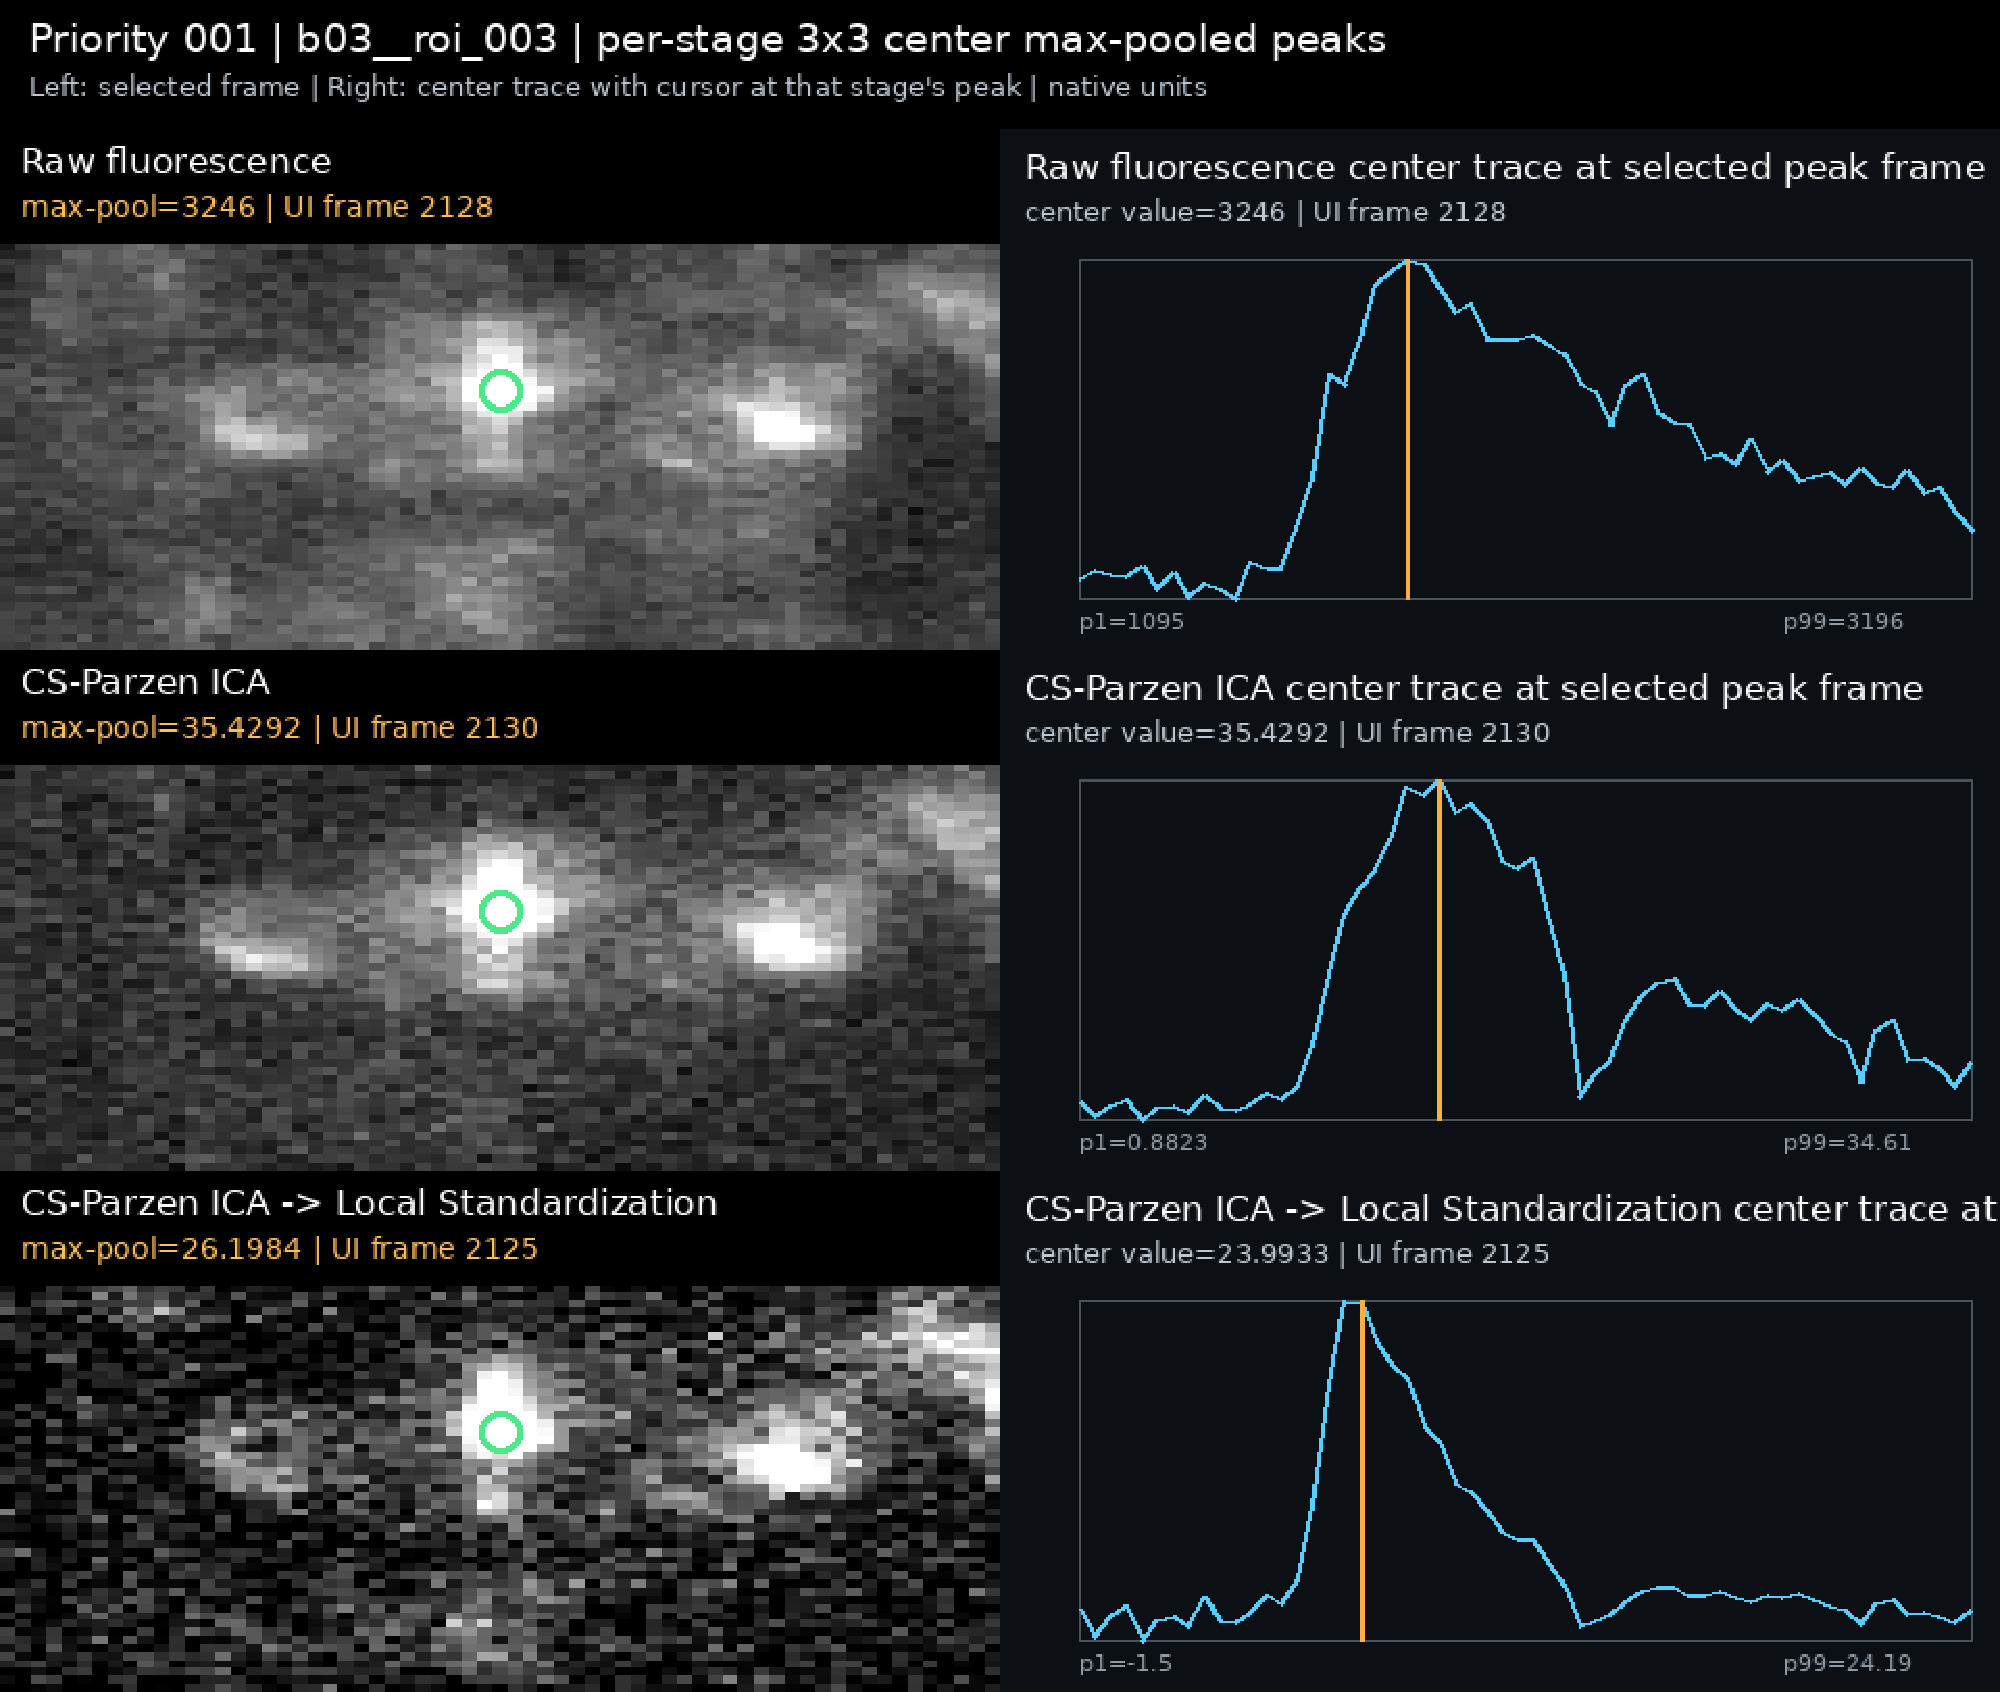
\includegraphics[page=1,width=0.98\linewidth]{figures/final/fig03_trace_atlas_examples.pdf}
  \caption{Frozen representative trace-atlas cases. (a) Hero: ROI~003 in burst~3, the frozen high-observability confirmed site. Left panels show each representation at its own $3\times3$ center max-pooled frame; right panels show the exact center trace with the selected frame marked. Values remain in representation-native units.}
  \label{fig:trace-atlas-cases}
\end{figure}

\begin{figure}[p]\ContinuedFloat
  \centering
  \includegraphics[page=2,width=0.98\linewidth]{figures/final/fig03_trace_atlas_examples.pdf}
  \caption{Frozen representative trace-atlas cases (continued). (b) Antihero: ROI~011 in burst~4, a confirmed but difficult observation site. ``Antihero'' denotes a hard known-positive case, not a negative or artifact.}
\end{figure}

\begin{figure}[p]\ContinuedFloat
  \centering
  \includegraphics[page=3,width=0.98\linewidth]{figures/final/fig03_trace_atlas_examples.pdf}
  \caption{Frozen representative trace-atlas cases (continued). (c) Random inclusion: ROI~010 in burst~3, selected from eligible confirmed four-burst sites with seed 20260824 before inspection of these panels. The original ROI~010 observation-site geometry is retained despite its provisional canonical merge with ROI~015.}
\end{figure}

\subsection{Trace reassessment supports two measurement profiles with incomplete stage preservation}

The reassessment in \Cref{fig:population-trace-summary} assigns all 50
coordinate-defined sites, representing 106 confirmed occurrences, from their
joint Raw, CS--Parzen ICA, and local-standardization trace shapes. The selected
two-class solution contained 38 and 12 sites. It had silhouette 0.261 and
median 80\% subsample adjusted Rand agreement 0.884, although the 10th
percentile agreement was 0.331. A three-class solution was admissible but had
lower silhouette (0.153) and median stability (0.727). Thus, two classes are
the preferred compact description, but the lower stability tail argues
against treating every site label as definitive.

Both classes show an onset-associated response. Trace Class~T1 has a more sustained
positive tail and higher native event peaks, whereas Trace Class~T2 returns toward or
below baseline more rapidly and has lower native peaks across the processed
representations. Amplitude was not used to fit these primary labels. Retaining
20 principal components reproduced the primary assignment exactly, and 12
components produced ARI 0.915; an eight-component compression was less stable
(ARI 0.358). Adding log native amplitude also changed assignments as its block
weight increased, confirming that shape and observability should remain
separate views rather than being collapsed into one nominal class.

\begin{figure}[p]
  \centering
  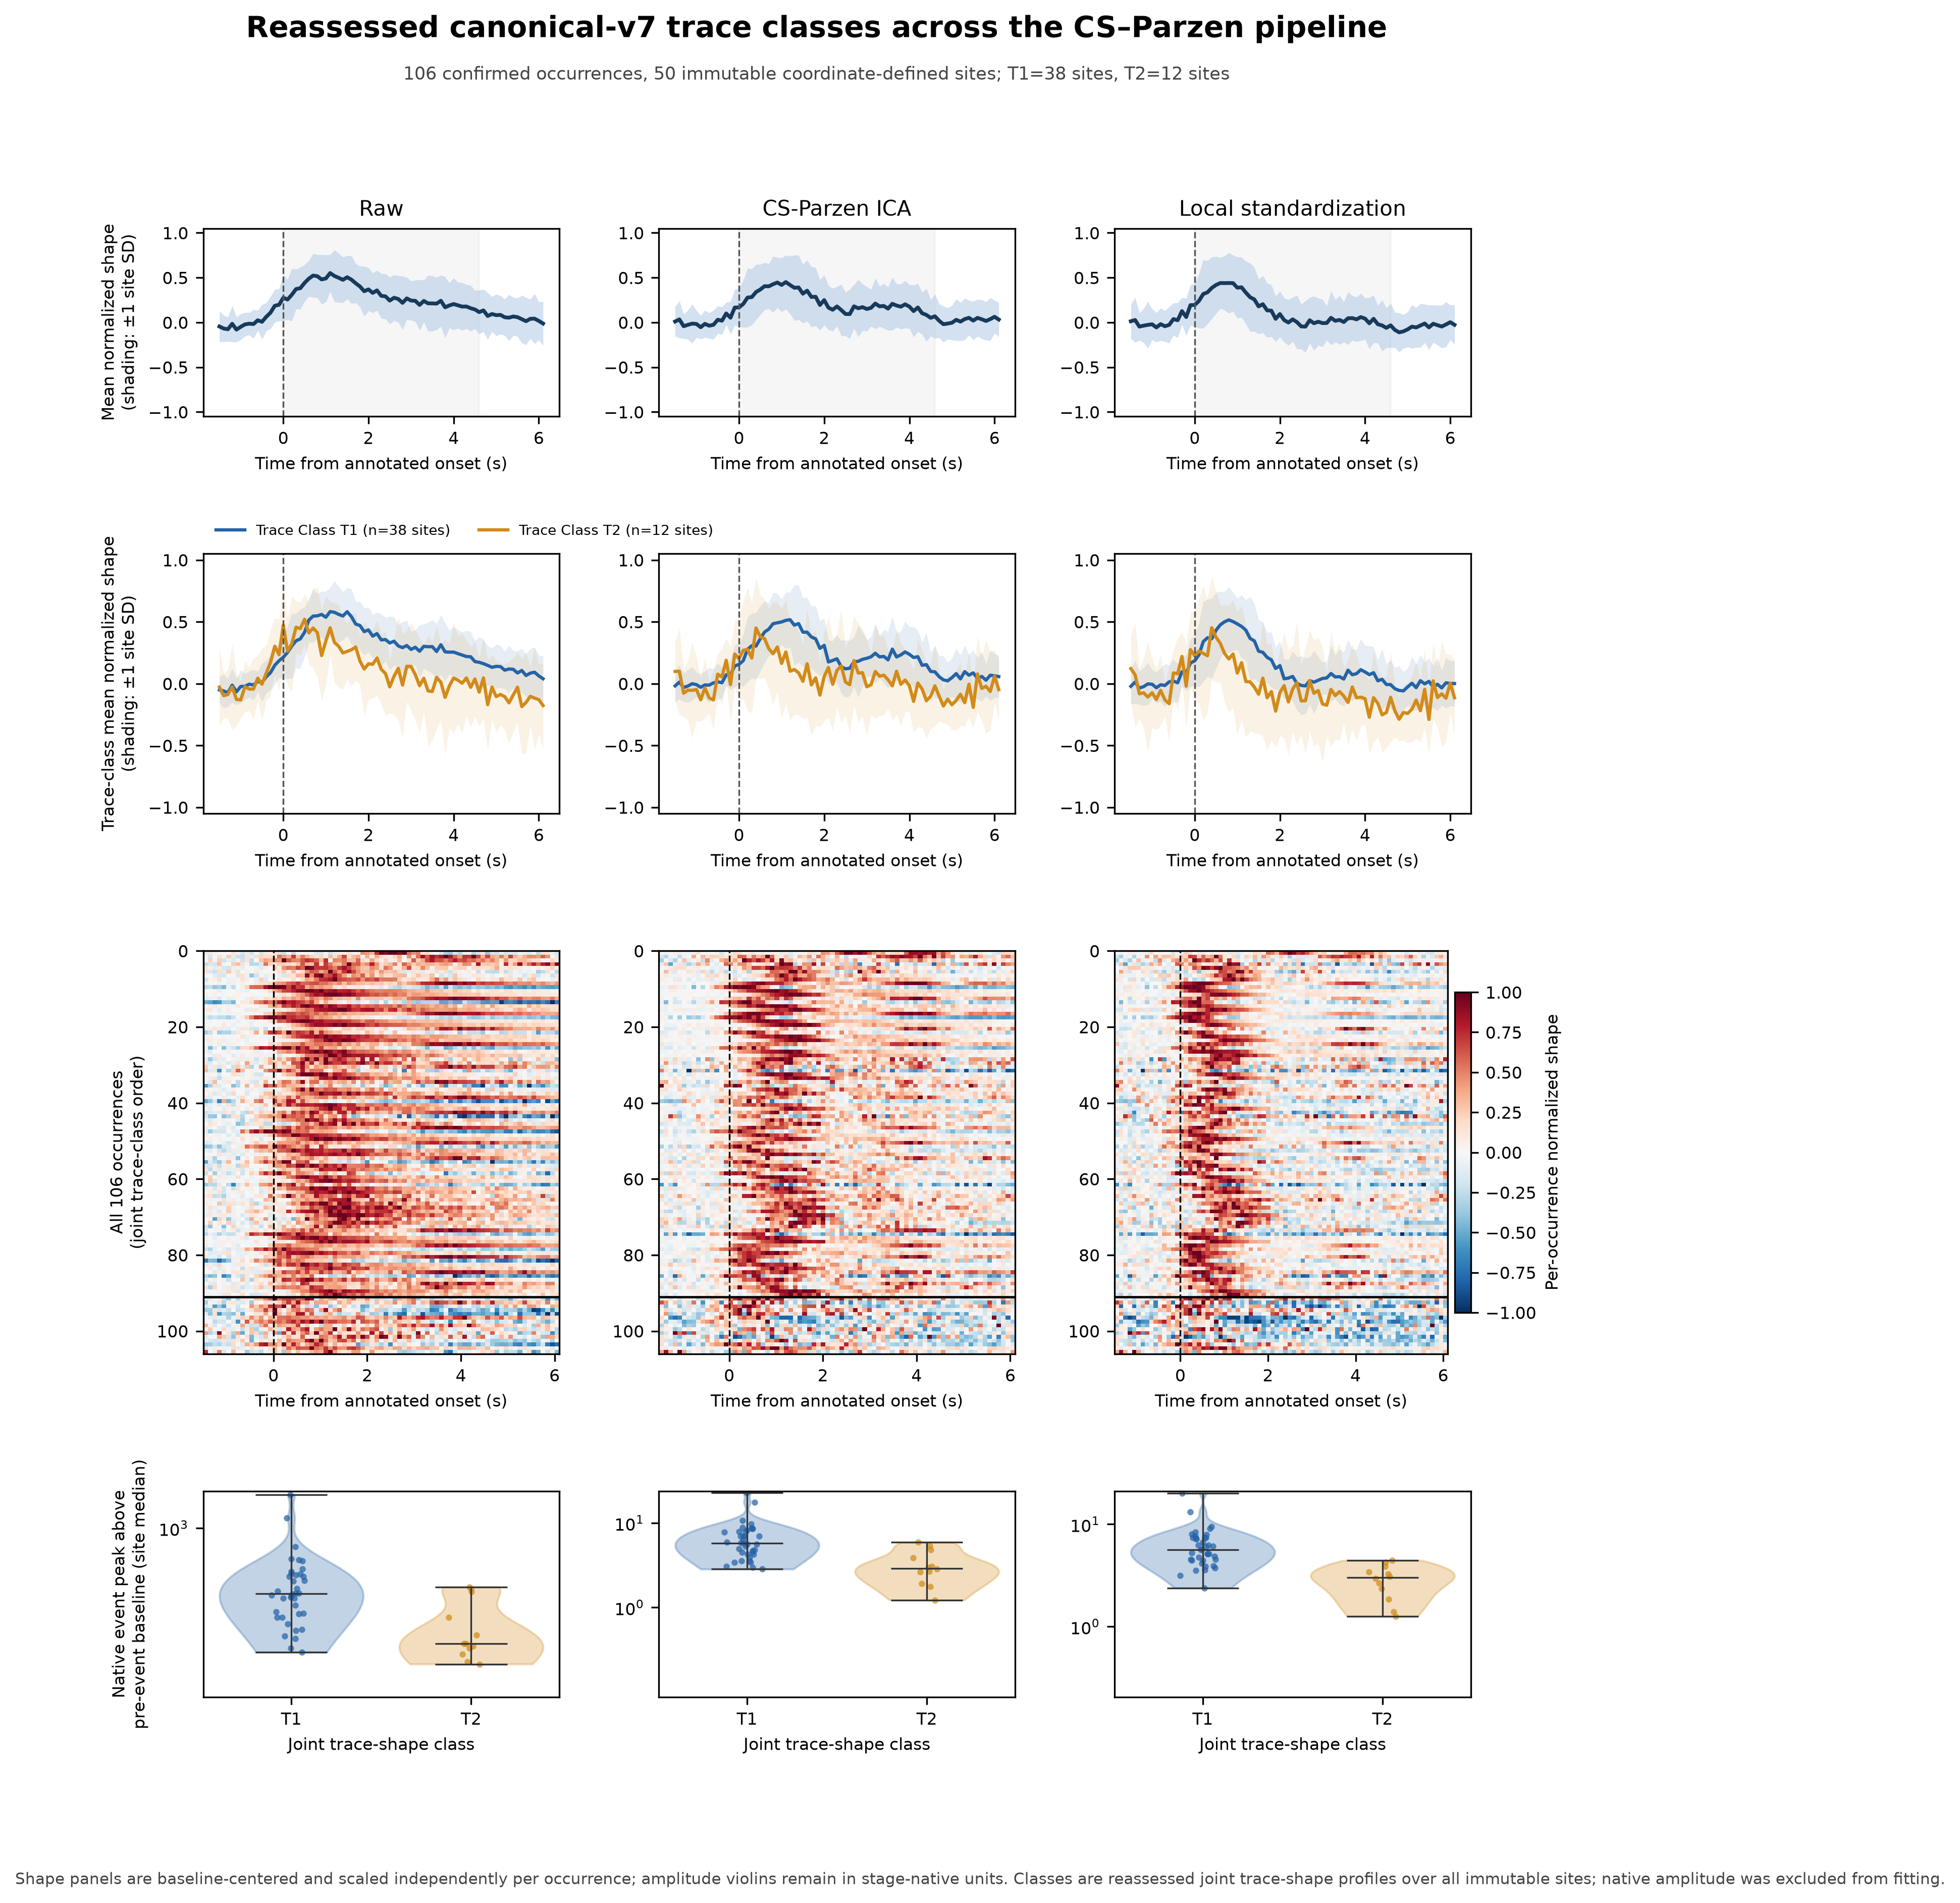
\includegraphics[width=0.98\linewidth]{figures/final/fig04_population_trace_summary.png}
  \caption{Reassessed population trace summary across Raw, CS--Parzen ICA, and local
  standardization. Top row: site-level mean normalized shape with $\pm1$
  site standard deviation. Second row: means and standard deviations for the
  two joint trace-shape classes. Third row: all confirmed occurrences in one
  fixed site/class order across representations; the heavy separator marks the
  class boundary. Bottom row: site-median native event-peak distributions,
  shown in representation-specific units. Traces
  are onset-aligned but not peak-aligned. Shape normalization is performed
  independently per occurrence and representation; the amplitude panels are
  not normalized across representations and amplitude was excluded from class
  fitting.}
  \label{fig:population-trace-summary}
\end{figure}

Independent stage fits did not preserve the smaller profile uniformly
(\Cref{fig:trace-taxonomy-stage-agreement}). Relative to the joint taxonomy,
Raw-only labels had ARI 0.578, CS--Parzen ICA-only labels 0.332, and
local-standardization-only labels 0.414. Every joint Trace Class~T1 site remained in
aligned stage Trace Class~T1, but only seven, four, and five of the 12 joint Trace Class~T2
sites were recovered by Raw, ICA, and local standardization, respectively.
Thirty-nine of 50 sites received the same aligned label in all three
stage-specific fits. This asymmetry suggests that the smaller joint profile is
defined partly by cross-stage information rather than by a stage-invariant
partition; it does not establish that the pipeline changes biological cell
identity.

\begin{figure}[!htbp]
  \centering
  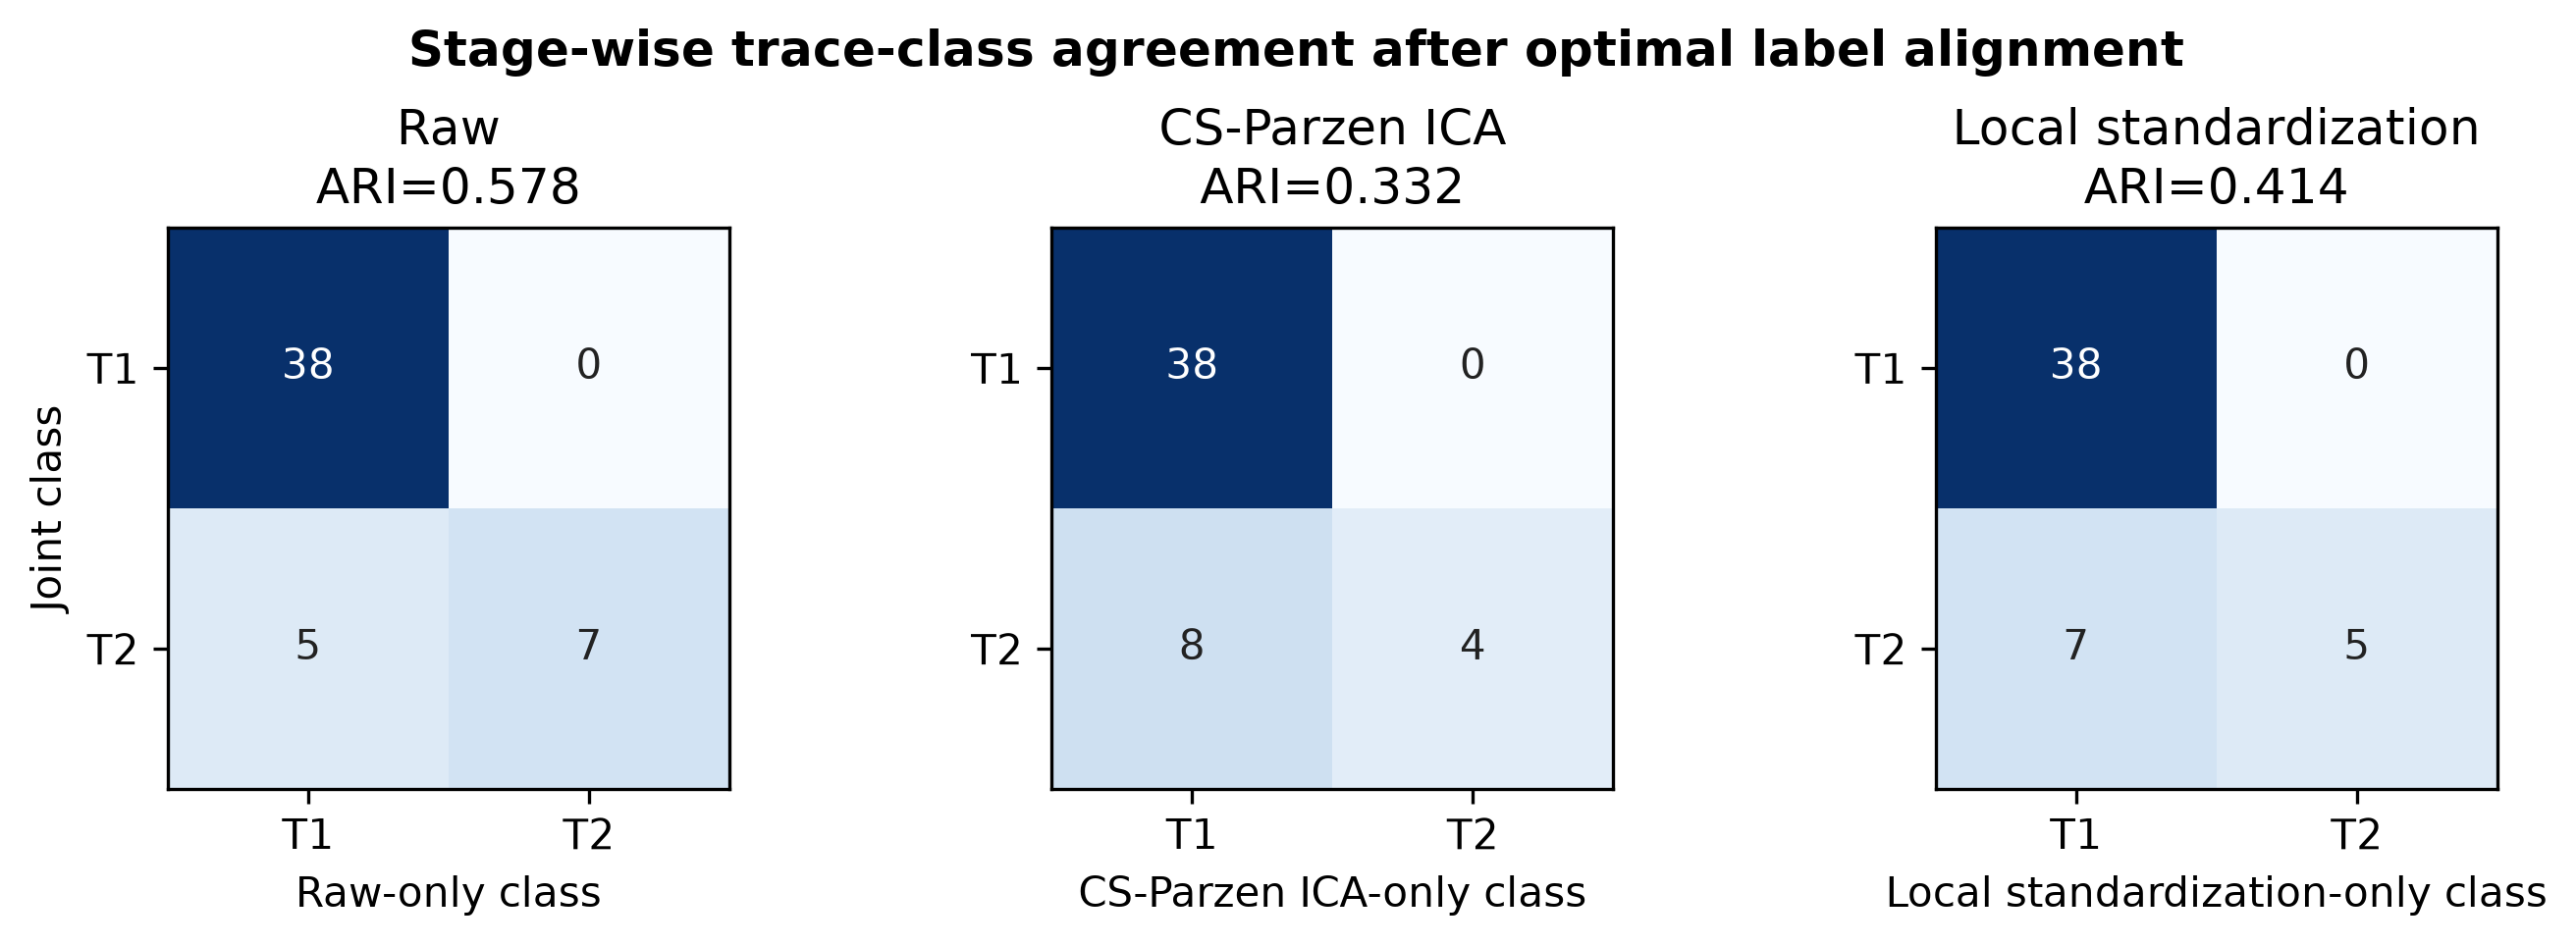
\includegraphics[width=0.98\linewidth]{figures/final/fig04b_trace_taxonomy_stage_agreement.png}
  \caption{Agreement between the joint two-class trace taxonomy and independent
  Raw-, CS--Parzen ICA-, and local-standardization-only fits. Labels were
  optimally permuted for display; adjusted Rand indices are permutation
  invariant. Counts are immutable coordinate-defined sites.}
  \label{fig:trace-taxonomy-stage-agreement}
\end{figure}

Leave-one-burst-out analysis favored a burst-dependent trace state over an
immutable site type (\Cref{fig:trace-taxonomy-lobo}). Eighty-one held-out
assignments from 25 recurrent sites were eligible. Site-blocked agreement with
the class learned from the other bursts was 0.740 (95\% bootstrap interval
0.647--0.833) and increased to 0.840 (0.740--0.927) when burst~2 was excluded.
Agreement by held-out burst was 0.824, 0.368, 0.708, and 1.000 for bursts
1--4, respectively. Only nine of 25 recurrent sites agreed with their
training-derived class in every available fold, and only three retained one
held-out label across all available bursts. The median centroid margin was
0.133, with 39.5\% of assignments below 0.10. Consequently, T1/T2 is retained
as a compact descriptive trace axis, but the evidence does not support two
immutable neuron classes. Burst state and boundary uncertainty are substantial,
with burst~2 the clearest source of instability.

\begin{figure}[p]
  \centering
  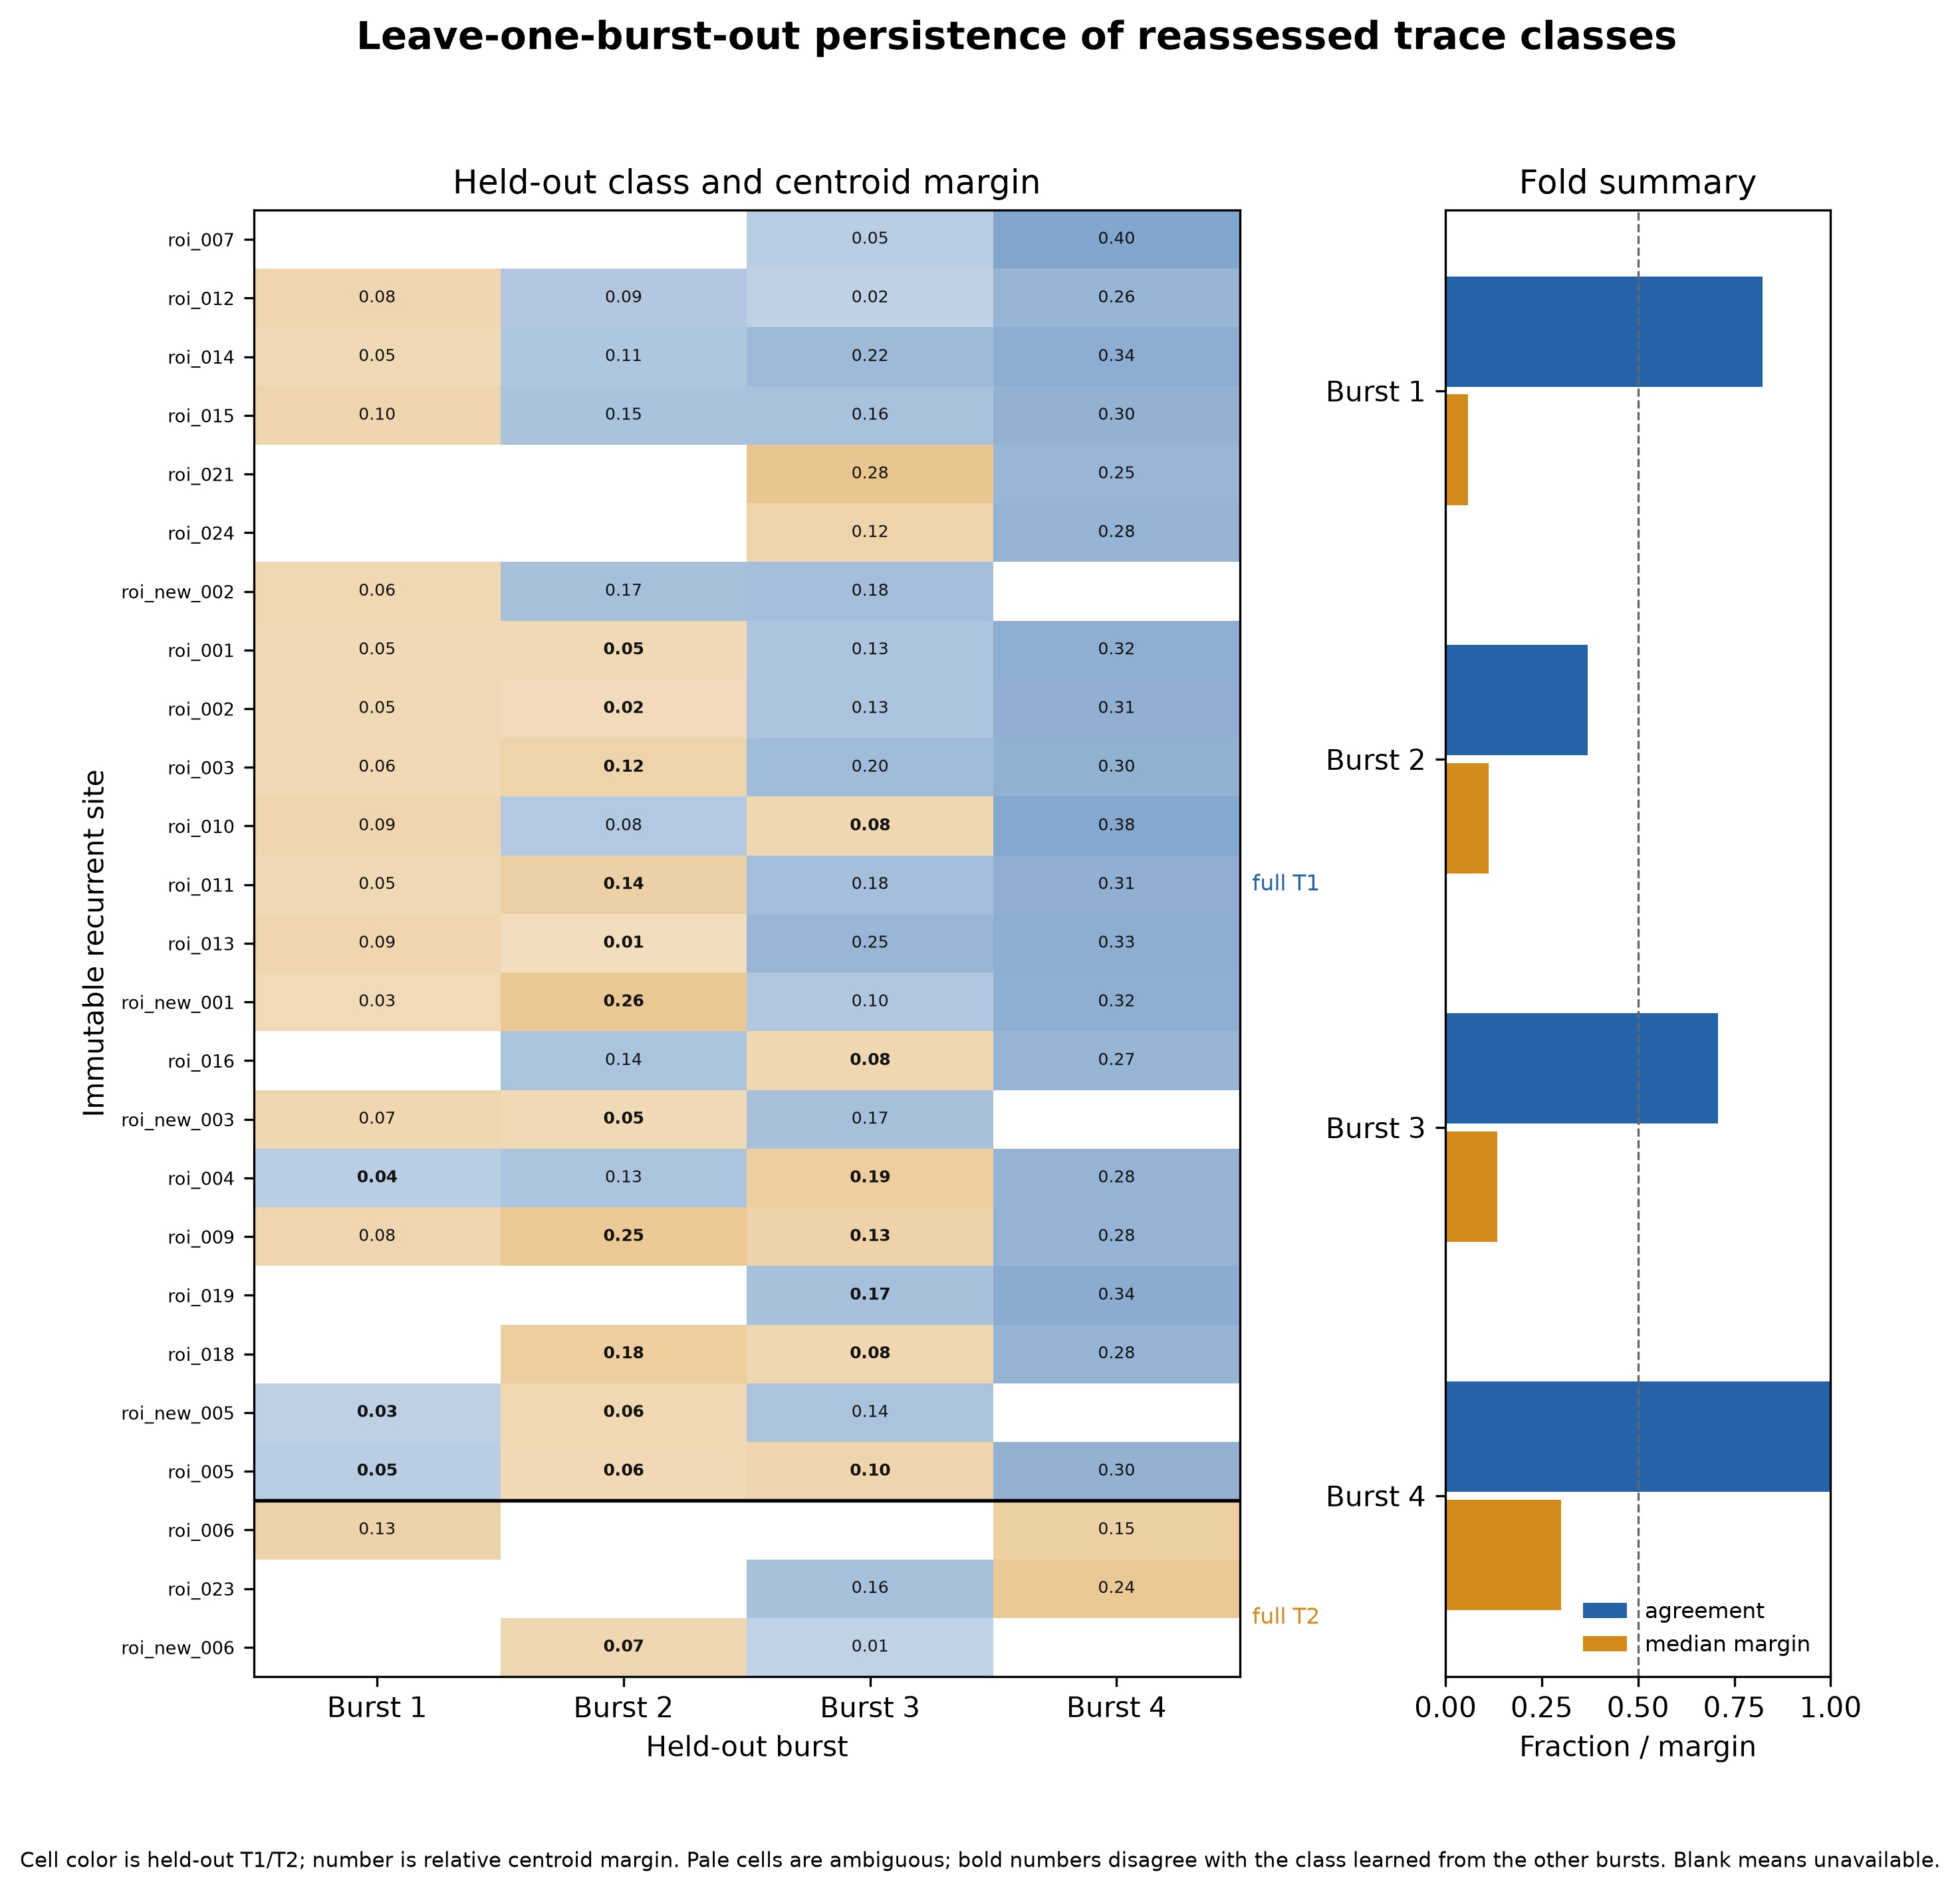
\includegraphics[width=0.98\linewidth]{figures/final/fig04c_trace_taxonomy_lobo_persistence.png}
  \caption{Leave-one-burst-out trace-class persistence for recurrent immutable
  sites. Cell color gives the held-out T1/T2 assignment and the printed value
  is the relative centroid margin; paler cells are closer to the boundary.
  Bold values disagree with the class learned from the other bursts. Blank
  cells indicate that the site was unavailable in that held-out burst. The
  side panel reports fold-level agreement and median margin.}
  \label{fig:trace-taxonomy-lobo}
\end{figure}

\subsection{The diagnostic audit separates transformation effects from missing model internals}

The audit contains 318 unique occurrence--stage rows (106 confirmed
occurrences by three representations) with no duplicate composite keys
(\Cref{fig:pipeline-diagnostic-audit}). Raw-to-ICA center traces had median
shape correlation 0.654 (10th--90th percentile 0.184--0.871) and median peak
shift $+0.2$~s. ICA-to-local-standardization traces were more similar (median
correlation 0.945, 10th--90th percentile 0.821--0.997) with median peak shift
zero. Median positive late-to-early persistence declined from 0.692 in Raw to
0.443 in ICA and 0.188 after local standardization. Thus the first transition
substantially changes waveform shape, whereas the second generally preserves
the immediate response while suppressing its late positive tail.

Burst~2 was also weak in native Raw measurements: its median peak was 283 and
median robust SNR 2.43, compared with peaks 352, 538, and 531 and SNRs 4.87,
8.79, and 10.08 in bursts 1, 3, and 4. This acquisition/event-strength
difference is consistent with, but does not by itself explain, the burst~2
class instability. Six of 106 local Raw crops contained at least one saturated
sample, but no labeled center trace reached the 4095 ceiling.

At the local-standardization stage, the binary T2 label was associated
descriptively with lower robust SNR ($\rho=-0.447$), lower center--annulus
contrast ($\rho=-0.353$), larger effective radius ($\rho=0.307$), and lower
center--annulus trace correlation ($\rho=-0.479$). Persistence itself had only
$\rho=0.188$ with the binary cut, reinforcing that the Ward partition is not a
threshold on one simple persistence statistic. These are post-fit descriptive
associations within one recording; trace-derived associations are not
independent validation.

The audit also identifies a more consequential information gap. Final Raw,
ICA, and local-standardization movies support temporal, neighborhood, and
spatial diagnostics, and candidate-match metadata cover 71 of 106 confirmed
occurrences. The saved output does not contain component activations or
contributions, mixing/unmixing matrices, learned filters, a compatible
reconstruction residual, the true local-standardization denominator, or a
motion field. At the time of the movie-only audit, component attribution and
denominator-failure explanations were therefore blocked.

\begin{figure}[p]
  \centering
  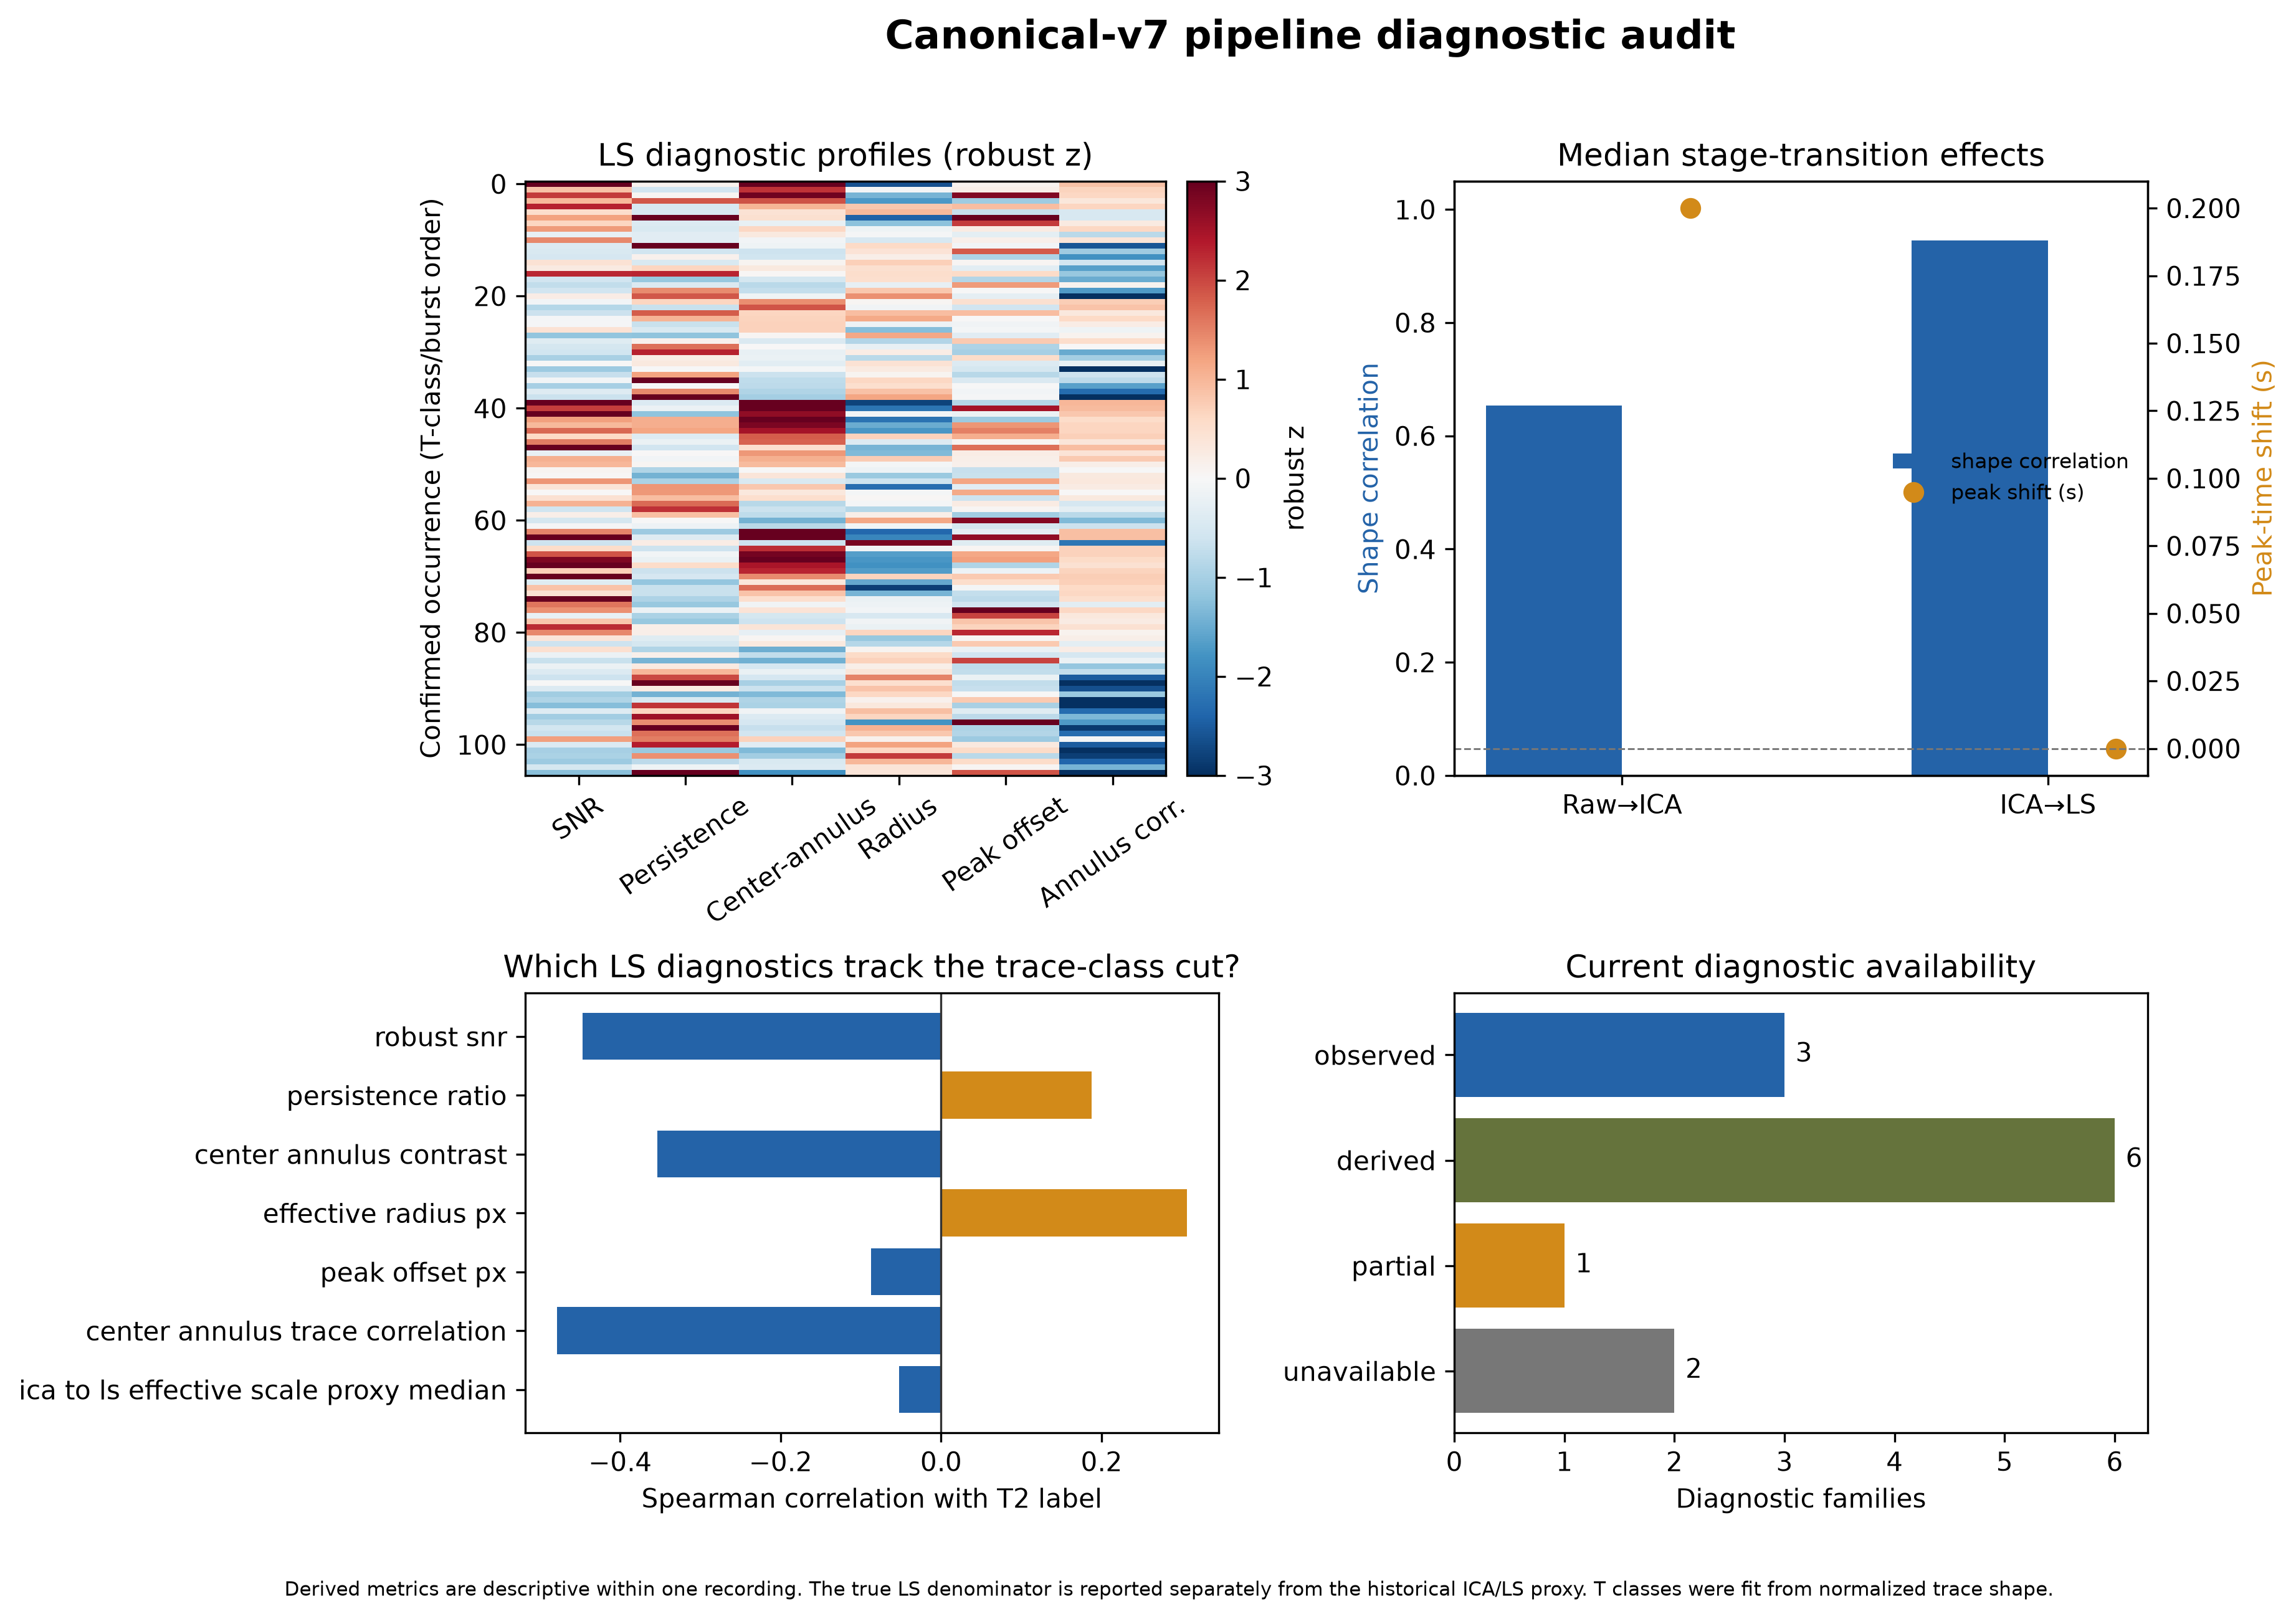
\includegraphics[width=0.98\linewidth]{figures/final/fig05_pipeline_diagnostic_audit.png}
  \caption{Canonical-v7 pipeline diagnostic audit. The heatmap shows robustly
  standardized local-standardization diagnostics for every confirmed
  occurrence. Stage-transition summaries use separate axes for trace
  correlation and peak-time shift. Correlations with T2 are descriptive and
  partially reuse trace information involved in class construction. The
  availability panel distinguishes observed, derived, partial, and unavailable
  diagnostic families.}
  \label{fig:pipeline-diagnostic-audit}
\end{figure}

The first model-internals refresh resolves the temporal-ICA portion of this gap
(\Cref{fig:ica-model-internals}). The frozen long-delay fit contains six
components over lags 0, 1, 2, 4, 8, and 16 frames; component~1 is the designated
persistence component, component~0 is innovation, and components~2--5 form the
reported residual group. Across all 50 unique sites, the full component traces,
mixing/demixing matrices, and energy fractions are now retained. The maximum
sitewise RMS embedding inversion residual was $5.69\times10^{-12}$, confirming
numerical invertibility at floating-point precision. This is deliberately not
reported as evidence of signal recovery or denoising quality. The true
local-standardization denominator is assessed separately below.

\begin{figure}[p]
  \centering
  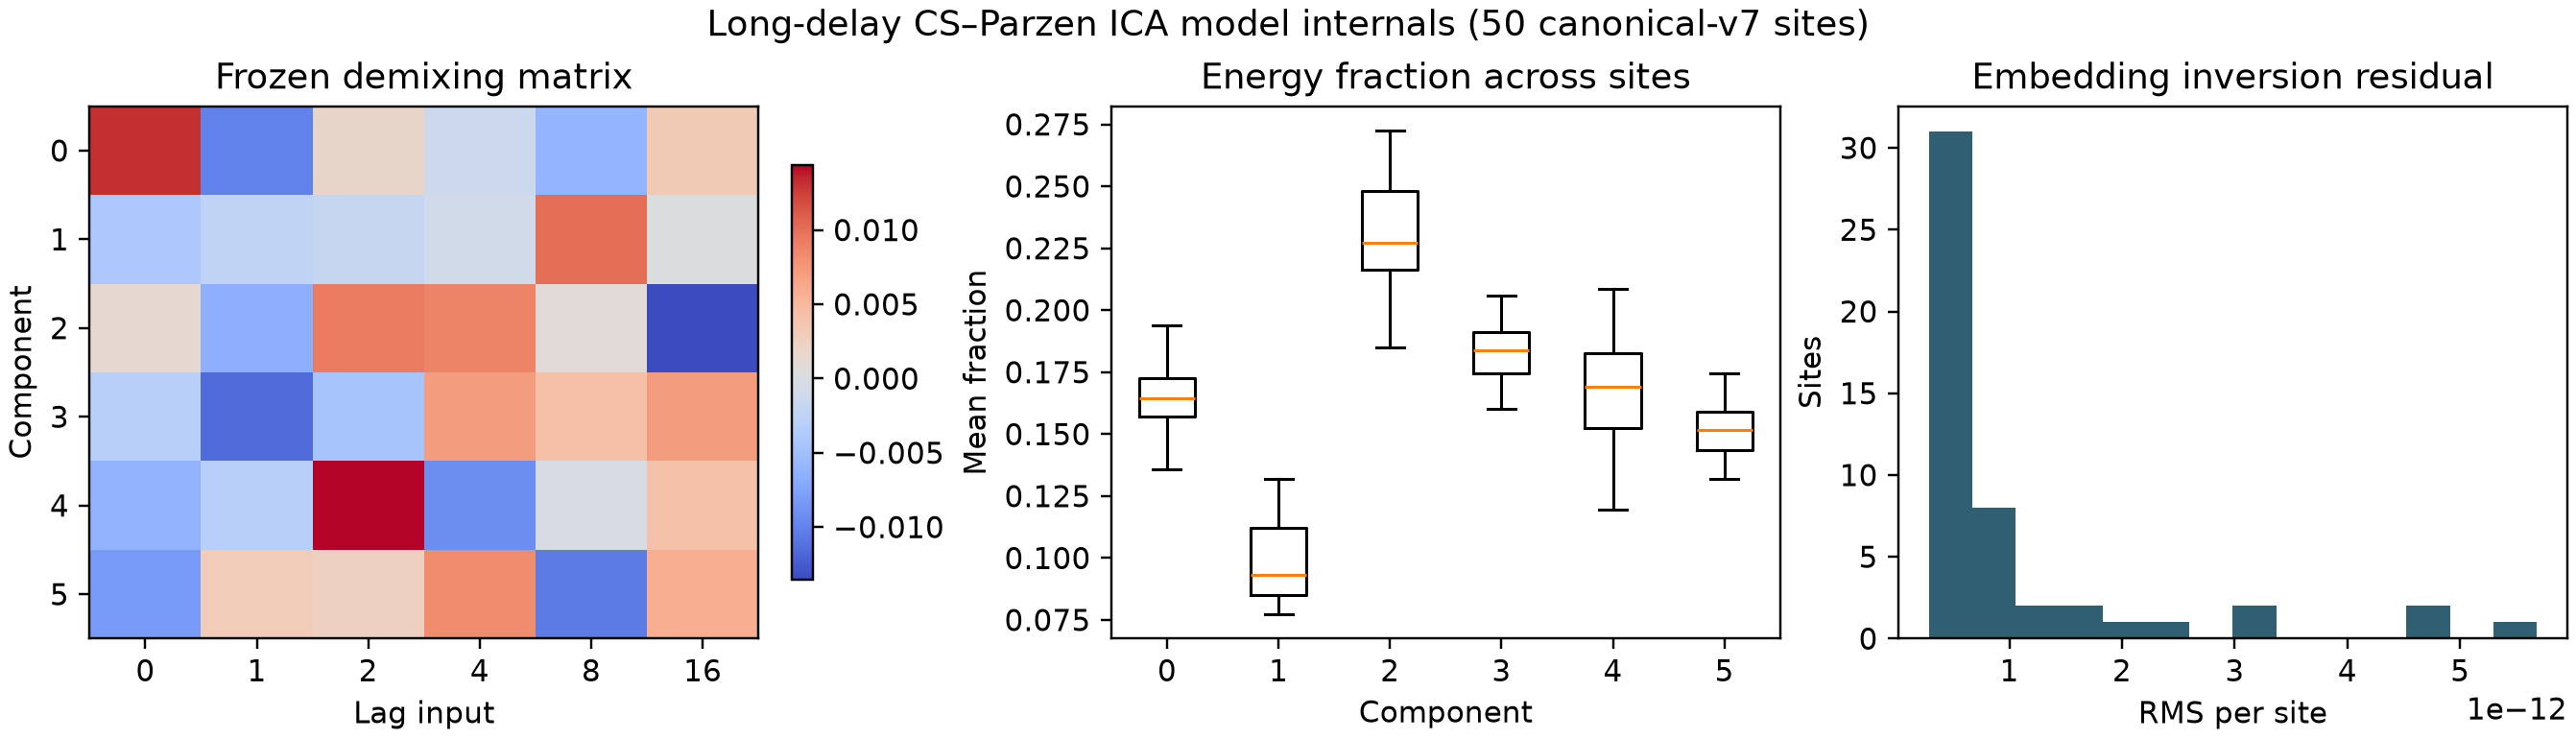
\includegraphics[width=0.98\linewidth]{figures/final/fig06_ica_model_internals.png}
  \caption{Frozen long-delay CS--Parzen ICA internals at the 50 unique
  canonical-v7 sites. Left, the learned demixing coefficients for lagged inputs.
  Middle, per-site temporal means of each component's squared-energy fraction.
  Right, numerical embedding inversion residuals. The right panel audits
  transform invertibility and is not a denoising-reconstruction metric.}
  \label{fig:ica-model-internals}
\end{figure}

The causal-pre-roll-preserving denominator audit reproduced the saved
local-standardization center traces with an overall RMS error of
$6.96\times10^{-7}$ and maximum absolute error of $7.63\times10^{-6}$
(\Cref{fig:ls-denominator-audit}). The frozen global scale floor was 0.371705,
whereas the median denominator across sites and frames was 0.7648. The floor
was not active at any of the 50 canonical-v7 centers during the 560-frame
review interval. Thus, center-trace amplification in this population is driven
by the measured local space--time scale rather than clipping to the global
floor. This does not rule out floor use elsewhere in the full field.

\begin{figure}[p]
  \centering
  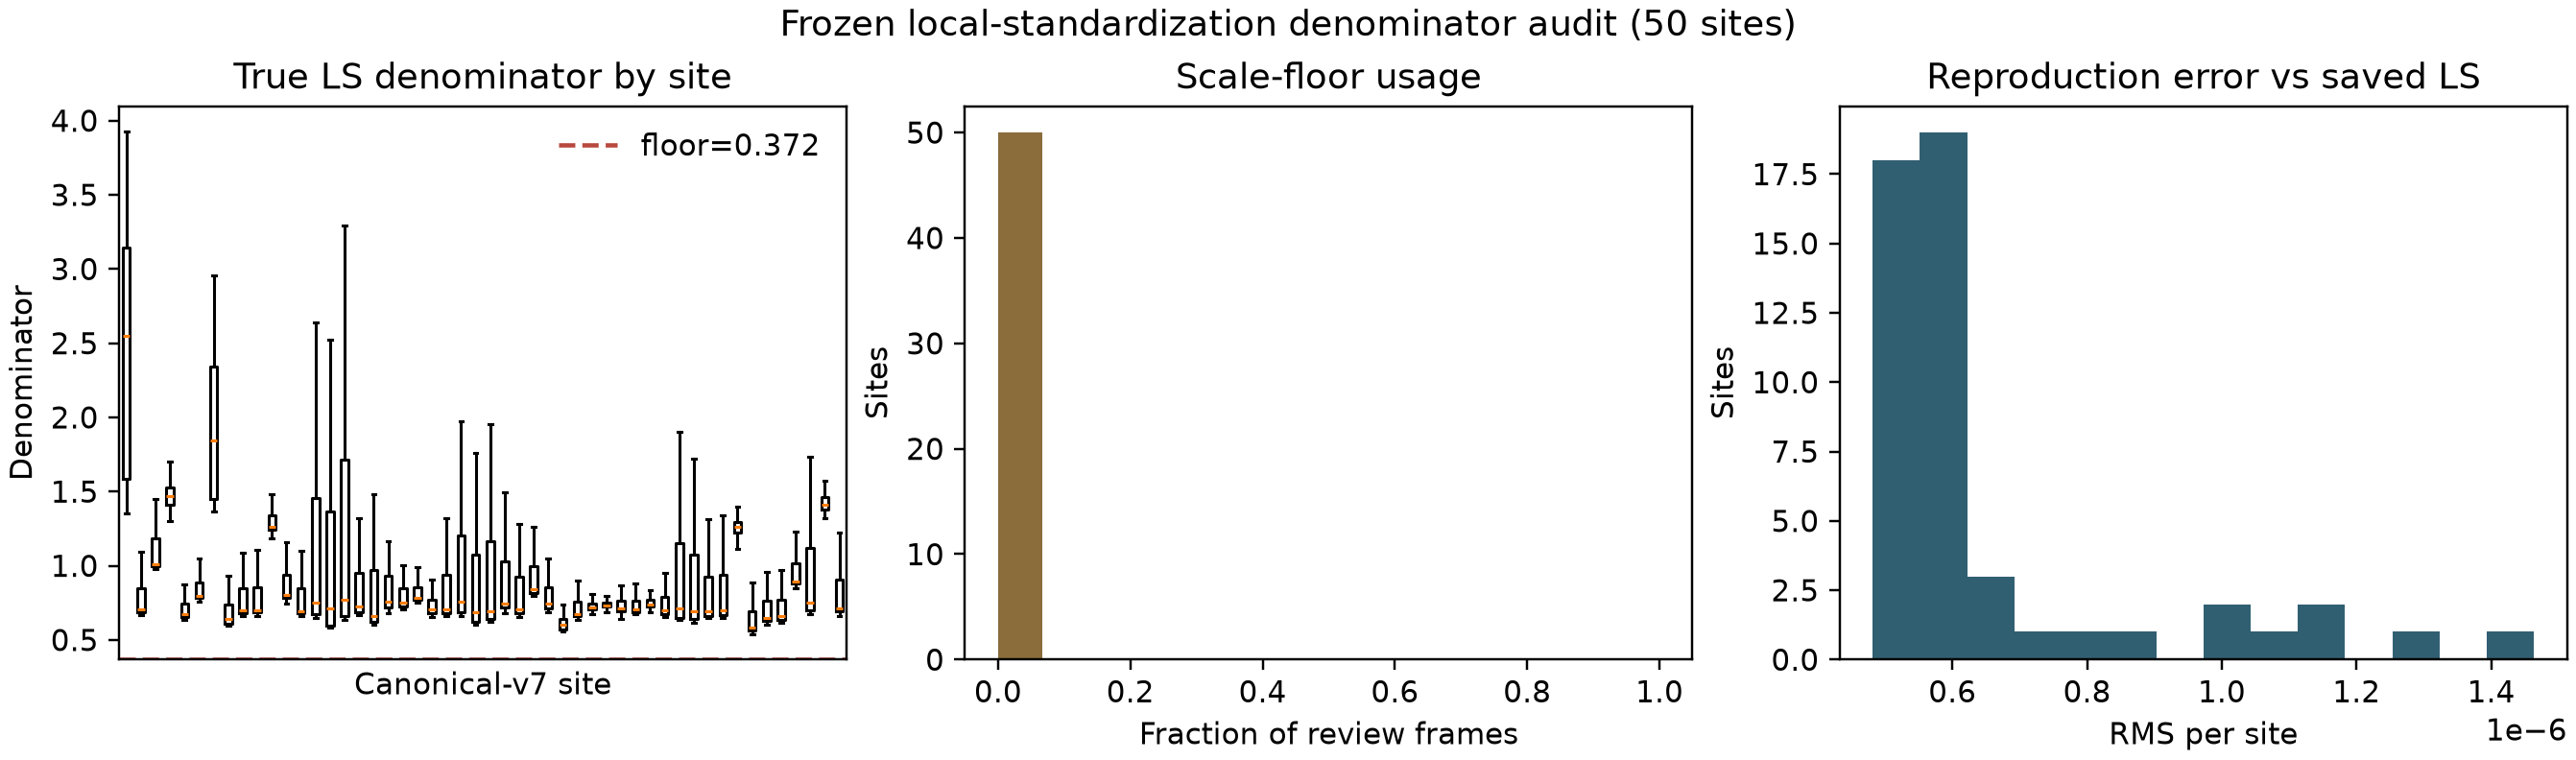
\includegraphics[width=0.98\linewidth]{figures/final/fig07_ls_denominator_diagnostics.png}
  \caption{Exact bounded reproduction of the frozen local-standardization
  denominator at 50 canonical-v7 sites. Left, denominator distributions by
  site with the saved global floor. Middle, the fraction of review frames for
  which the floor was active. Right, numerical agreement between reproduced
  and saved local-standardization center traces.}
  \label{fig:ls-denominator-audit}
\end{figure}

\subsection{Spatial/contextual features improve known-positive ranking without identifying precision}

In the earlier 79-observation full-field screen, carrier-only known-positive
recall at candidate budget 20 was \CarrierRecallBtwenty{}, compared with
\CoherenceRecallBtwenty{} for the cross-fitted local-coherence family and
\Provisional{0.5886} for the cross-fitted lagged-recurrence family. The exact
lag-2/15 lane reached the higher descriptive, post-hoc value
\LagRecallBtwenty{}. These values indicate that spatial and temporal context can
improve the ordering or proposal coverage of known positives. They do not
identify full-field precision because unmatched candidates may be unlabeled
neurons. The protected confirmation will hold proposals and non-maximum
suppression fixed where possible, separate proposal from ranking gains, and
reserve precision estimation for the exhaustively reviewed bounded field.

The complete-trace panel clarified why those contextual features should not be
treated as universal replacements for amplitude. At already confirmed centers,
the frozen carrier attained a site-weighted mean event-localization percentile
of \FullTraceCarrierPercentile{} (95\% site-bootstrap interval
\FullTraceCarrierCILow{}--\FullTraceCarrierCIHigh{}), while Raw, 15-frame
coherence, and lag-2 recurrence attained \FullTraceRawPercentile{},
\FullTraceCoherencePercentile{}, and \FullTraceLagPercentile{}, respectively.
The lagged score's paired difference from the carrier was only
\FullTraceLagDelta{} (95\% interval \FullTraceLagDeltaLow{}--
\FullTraceLagDeltaHigh{}) and did not pass the strictly positive interval gate.
The primary statistic was visibly ceiling-limited: \FullTraceCarrierCeilingCount{}/
\FullTraceOccurrences{} carrier scores, \FullTraceCoherenceCeilingCount{}/
\FullTraceOccurrences{} coherence scores, and \FullTraceLagCeilingCount{}/
\FullTraceOccurrences{} lag scores were exactly 1.0.

Neither prespecified extension improved localization over the carrier. The
Raw/ICA/local-standardization consensus reached
\FullTraceConsensusPercentile{}, and multiscale persistence reached
\FullTracePersistencePercentile{}. They did, however, retain cross-burst
site-rank variation after the strongest amplitude features saturated: median
available burst-pair Spearman correlations were
\FullTraceConsensusRepeatability{} and
\FullTracePersistenceRepeatability{}. Conversely, variance-stabilized
center-minus-annulus contrast reached \FullTraceVSTPercentile{}, supporting its
use as a noise/local-contamination diagnostic rather than the primary event
carrier. Thus the combined evidence assigns features to different roles:
amplitude for event strength at a known center, coherence for proposal and
early-budget ranking, recurrence as secondary temporal context, and
consensus/persistence as exploratory observability features.

\begin{table}[!htbp]
\centering
\scriptsize
\begin{tabularx}{\linewidth}{X r r r}
\toprule
Feature & Mean percentile [95\% CI] & $\Delta$ vs carrier & Median $\rho$ \\
\midrule
Raw center & 0.991 [0.973, 1.000] & -0.003 & -- \\
CS-Parzen ICA center & 0.964 [0.927, 0.992] & -0.030 & -- \\
Local standardization center & 0.935 [0.894, 0.969] & -0.059 & 0.524 \\
Raw center-annulus & 0.907 [0.857, 0.949] & -0.086 & 0.377 \\
VST center-annulus & 0.883 [0.824, 0.934] & -0.111 & 0.492 \\
LS exponential matched filter & 0.958 [0.918, 0.990] & -0.036 & -- \\
Frozen amplitude carrier & 0.994 [0.981, 1.000] & +0.000 & -- \\
Local coherence (15 frames) & 0.994 [0.981, 1.000] & +0.000 & -- \\
Lag-2 recurrence (15 frames) & 0.996 [0.987, 1.000] & +0.002 & -- \\
Raw/ICA/LS consensus & 0.986 [0.963, 0.999] & -0.008 & 0.633 \\
LS multiscale persistence & 0.972 [0.945, 0.992] & -0.022 & 0.649 \\
\bottomrule
\end{tabularx}
\caption{Exploratory full-trace feature panel at confirmed ROI centers. Percentiles compare each confirmed event maximum with all same-duration quiet-window maxima at the same immutable site; intervals use a 5,000-draw site bootstrap. The final column is the median available burst-pair Spearman correlation of site ranks; dashes denote ceiling-induced undefined correlations.}
\label{tab:full-trace-feature-panel}
\end{table}


\begin{figure}[p]
  \centering
  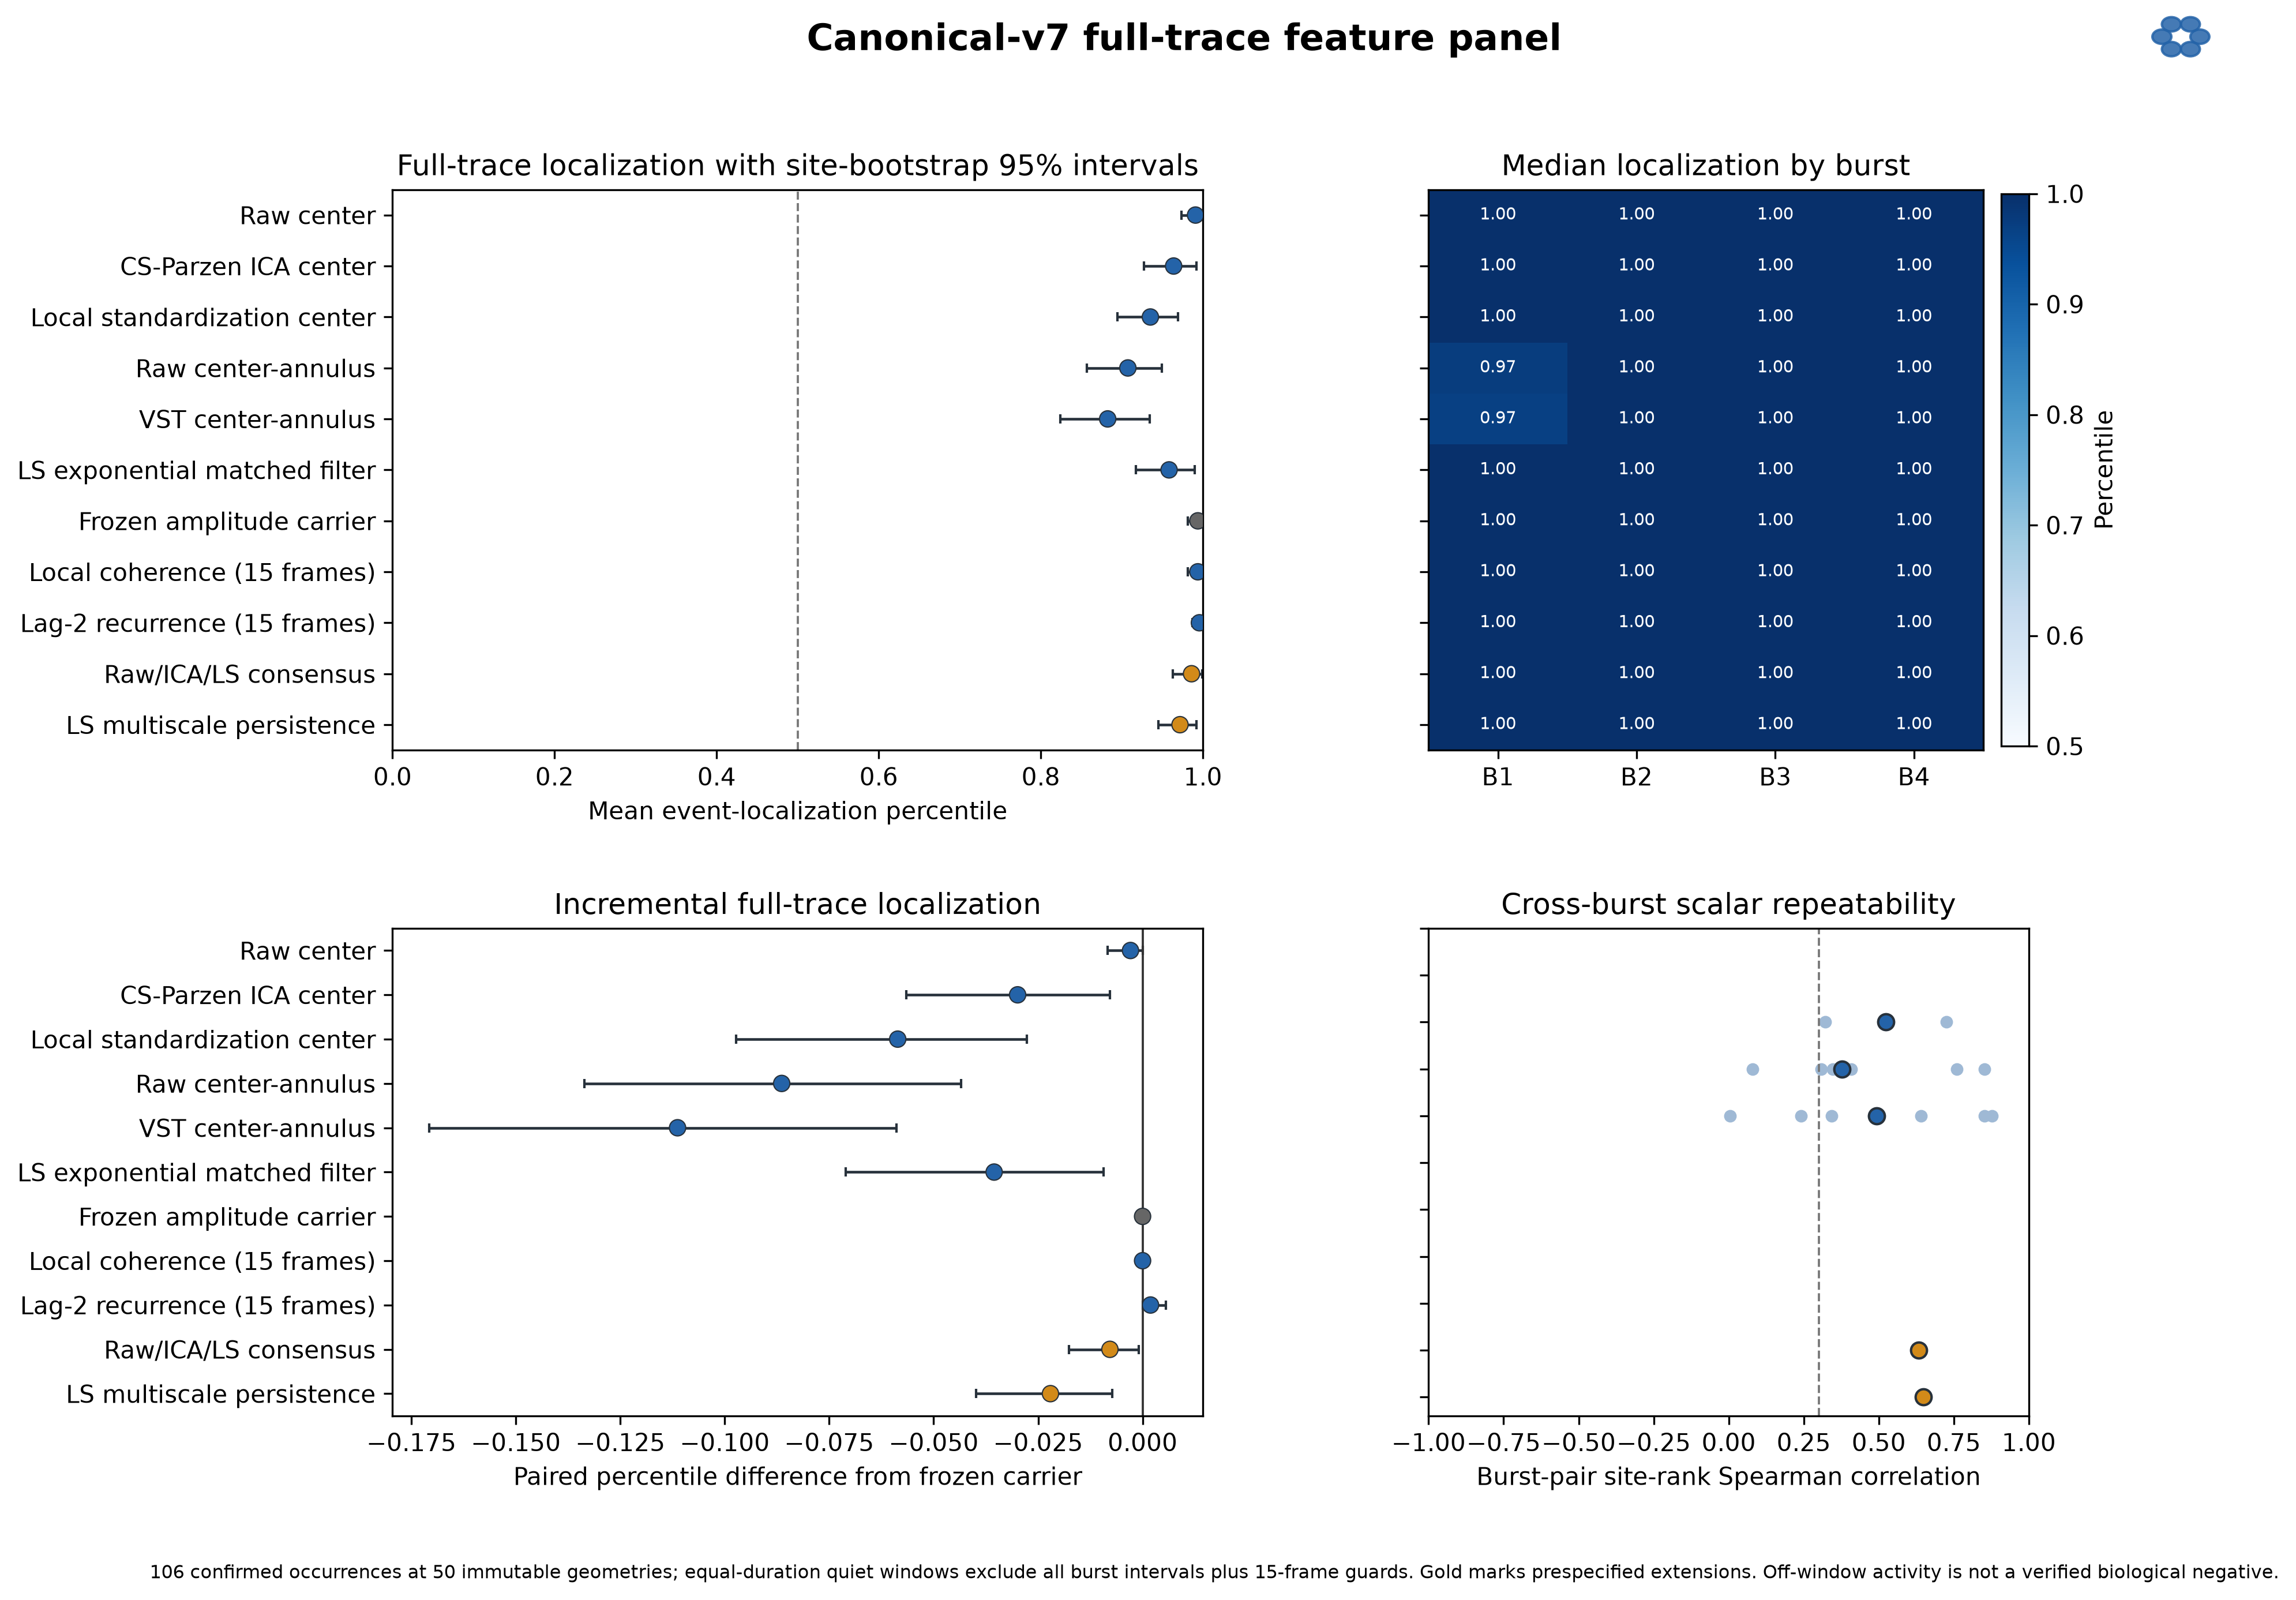
\includegraphics[width=0.98\linewidth]{figures/final/fig08_full_trace_feature_panel.png}
  \caption{Exploratory complete-trace feature panel for 106 confirmed
  occurrences at 50 immutable sites. Event maxima are compared with all
  same-duration guarded quiet-window maxima at the same site. Gold points are
  prespecified extensions. Undefined rank correlations arise when a burst is
  constant at the localization ceiling; quiet windows are not verified
  biological negatives.}
  \label{fig:full-trace-feature-panel}
\end{figure}

\subsection{Automated challenges support localized feature roles but not confirmed complementarity}

Replacing event maxima with frame-level event-versus-quiet retrieval removed
the earlier ceiling. Raw was strongest at \AutoRawAUC{} (95\% site-bootstrap
interval \AutoRawAUCLow{}--\AutoRawAUCHigh{}), followed by the carrier
(\AutoCarrierAUC{}), coherence (\AutoCoherenceAUC{}), lag-2 recurrence
(\AutoLagAUC{}), and the exponential matched filter (\AutoMatchedAUC{}).
All six compact spatial-challenge features had positive true-minus-displaced
AUC intervals. Multiscale persistence showed the largest paired difference,
\AutoPersistenceSpatialDelta{}, but its absolute temporal retrieval and
coordinate-jitter tolerance were lower than the amplitude/context lanes.

At budget 58, \AutoRecoveryCount{}/\FullTraceOccurrences{} original geometries
were recovered by at least one quantitative lane and \AutoRecoveryMisses{} were
missed. The carrier-only site-grouped model had cross-fitted log loss
\AutoCarrierLogLoss{} and ROC AUC 0.605; the role-specific model reached log
loss \AutoExtendedLogLoss{} and ROC AUC 0.826. The log-loss improvement was
\AutoRecoveryDelta{}, but its site-bootstrap interval was
\AutoRecoveryDeltaLow{}--\AutoRecoveryDeltaHigh{} and crossed zero. The
canonical-collapsed 102-row sensitivity was directionally similar, so the
feature panel is promising for error stratification but does not pass the
prespecified complementarity gate.

Reliability and event utility were not interchangeable. Raw center-annulus had
a site variance fraction of \AutoAnnulusReliability{} despite weak temporal
retrieval, whereas the carrier combined strong retrieval with a lower fraction
of \AutoCarrierReliability{}. All selected observed alignments exceeded 500
site-blocked circular shifts (minimum attainable upper-tail
$p=\AutoNullP{}$). Synthetic injections showed monotonic response; the matched
filter rose from mean AUC 0.531 at zero injection to 0.933 at four quiet-MAD
units, exceeding LS amplitude and persistence. These outcomes validate temporal
alignment and operator sensitivity, not neuron identity.

\begin{table}[!htbp]
\centering
\scriptsize
\begin{tabularx}{\linewidth}{X r r r}
\toprule
Feature & Frame AUC [95\% CI] & Spatial $\Delta$ AUC & Site fraction \\
\midrule
Raw center & 0.931 [0.906, 0.952] & 0.147 & 0.510 \\
Frozen amplitude carrier & 0.920 [0.896, 0.941] & 0.152 & 0.580 \\
Local coherence (15 frames) & 0.915 [0.890, 0.938] & 0.171 & 0.741 \\
Lag-2 recurrence (15 frames) & 0.905 [0.878, 0.927] & 0.169 & 0.735 \\
LS exponential matched filter & 0.884 [0.843, 0.917] & -- & 0.687 \\
Raw/ICA/LS consensus & 0.803 [0.776, 0.828] & 0.152 & 0.756 \\
LS multiscale persistence & 0.780 [0.742, 0.817] & 0.217 & 0.770 \\
Raw center-annulus & 0.727 [0.685, 0.773] & -- & 0.866 \\
\bottomrule
\end{tabularx}
\caption{Automated full-trace validation. Frame AUC separates annotated event frames from guarded quiet-reference frames. Spatial differences compare the true center with same-field baseline-matched displaced tissue. Site fraction is a nonparametric variance fraction, not REML ICC. Quiet and displaced references have unknown biological labels.}
\label{tab:automated-feature-validation}
\end{table}


\begin{figure}[p]
  \centering
  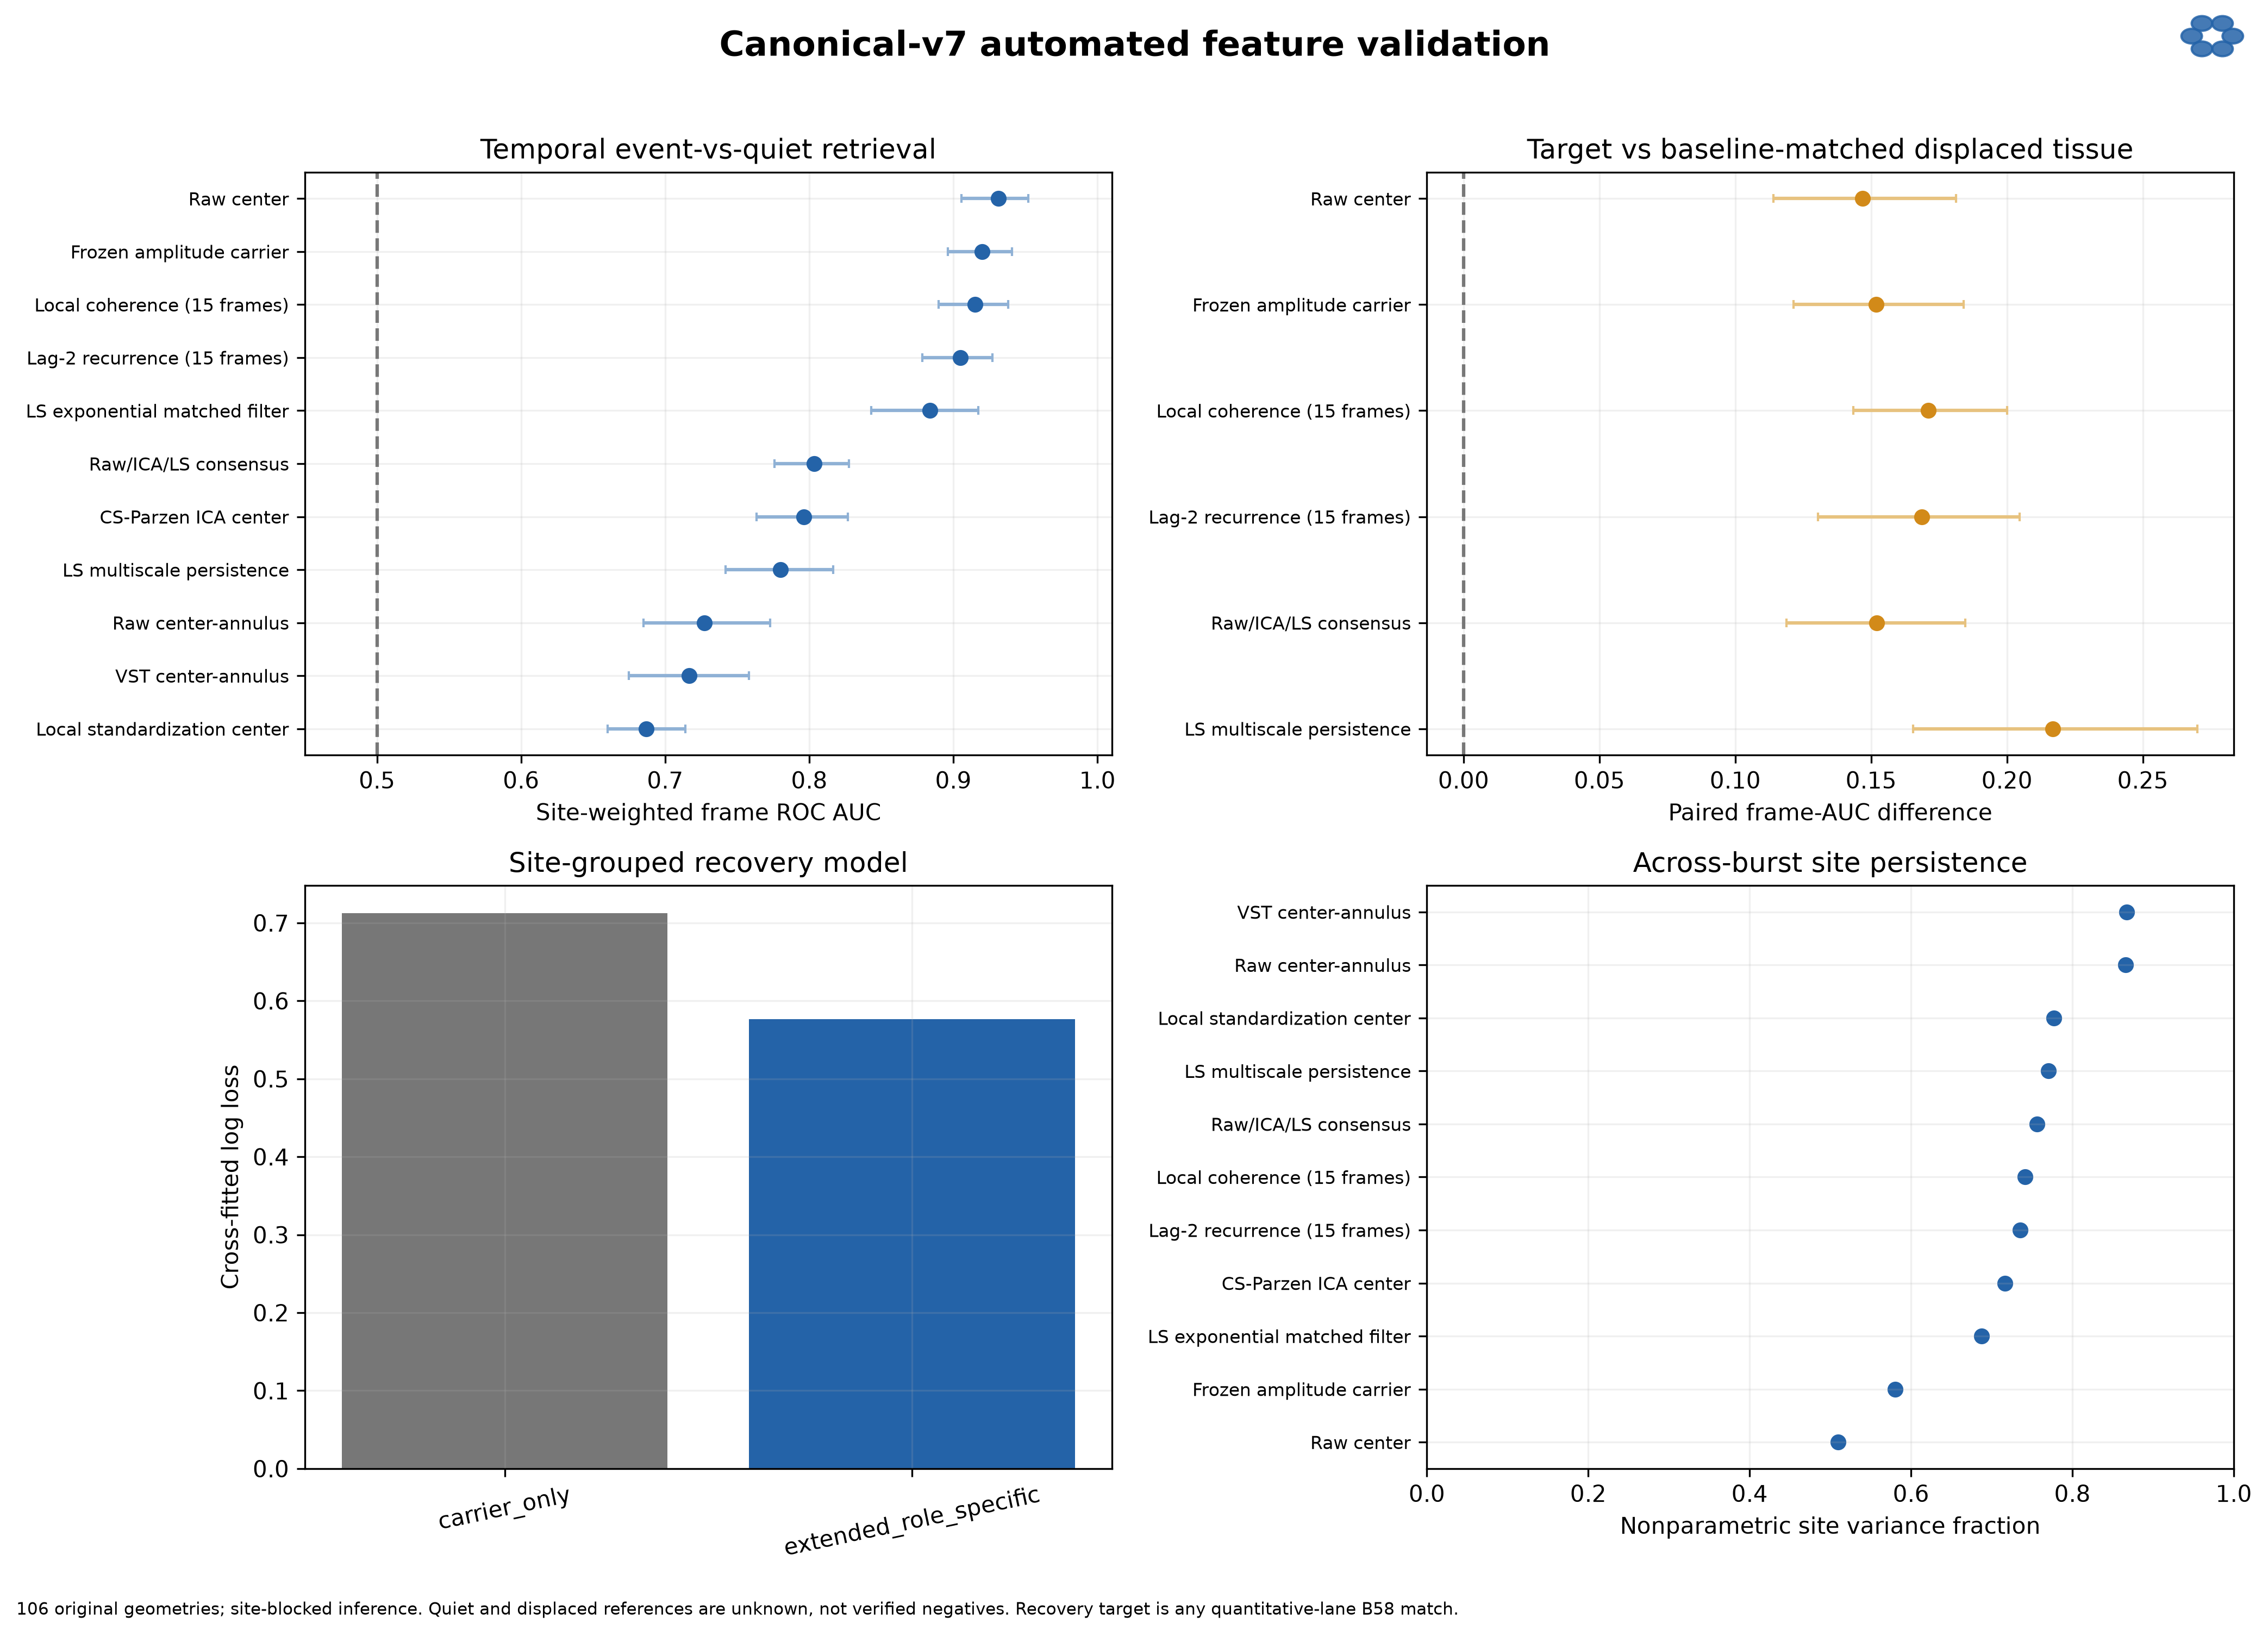
\includegraphics[width=0.98\linewidth]{figures/final/fig09_automated_feature_validation.png}
  \caption{Automated temporal retrieval, spatial displacement, grouped
  recoverability, and repeatability tests. Displaced tissue is an unknown
  control, not a verified negative.}
  \label{fig:automated-feature-validation}
\end{figure}

\begin{figure}[p]
  \centering
  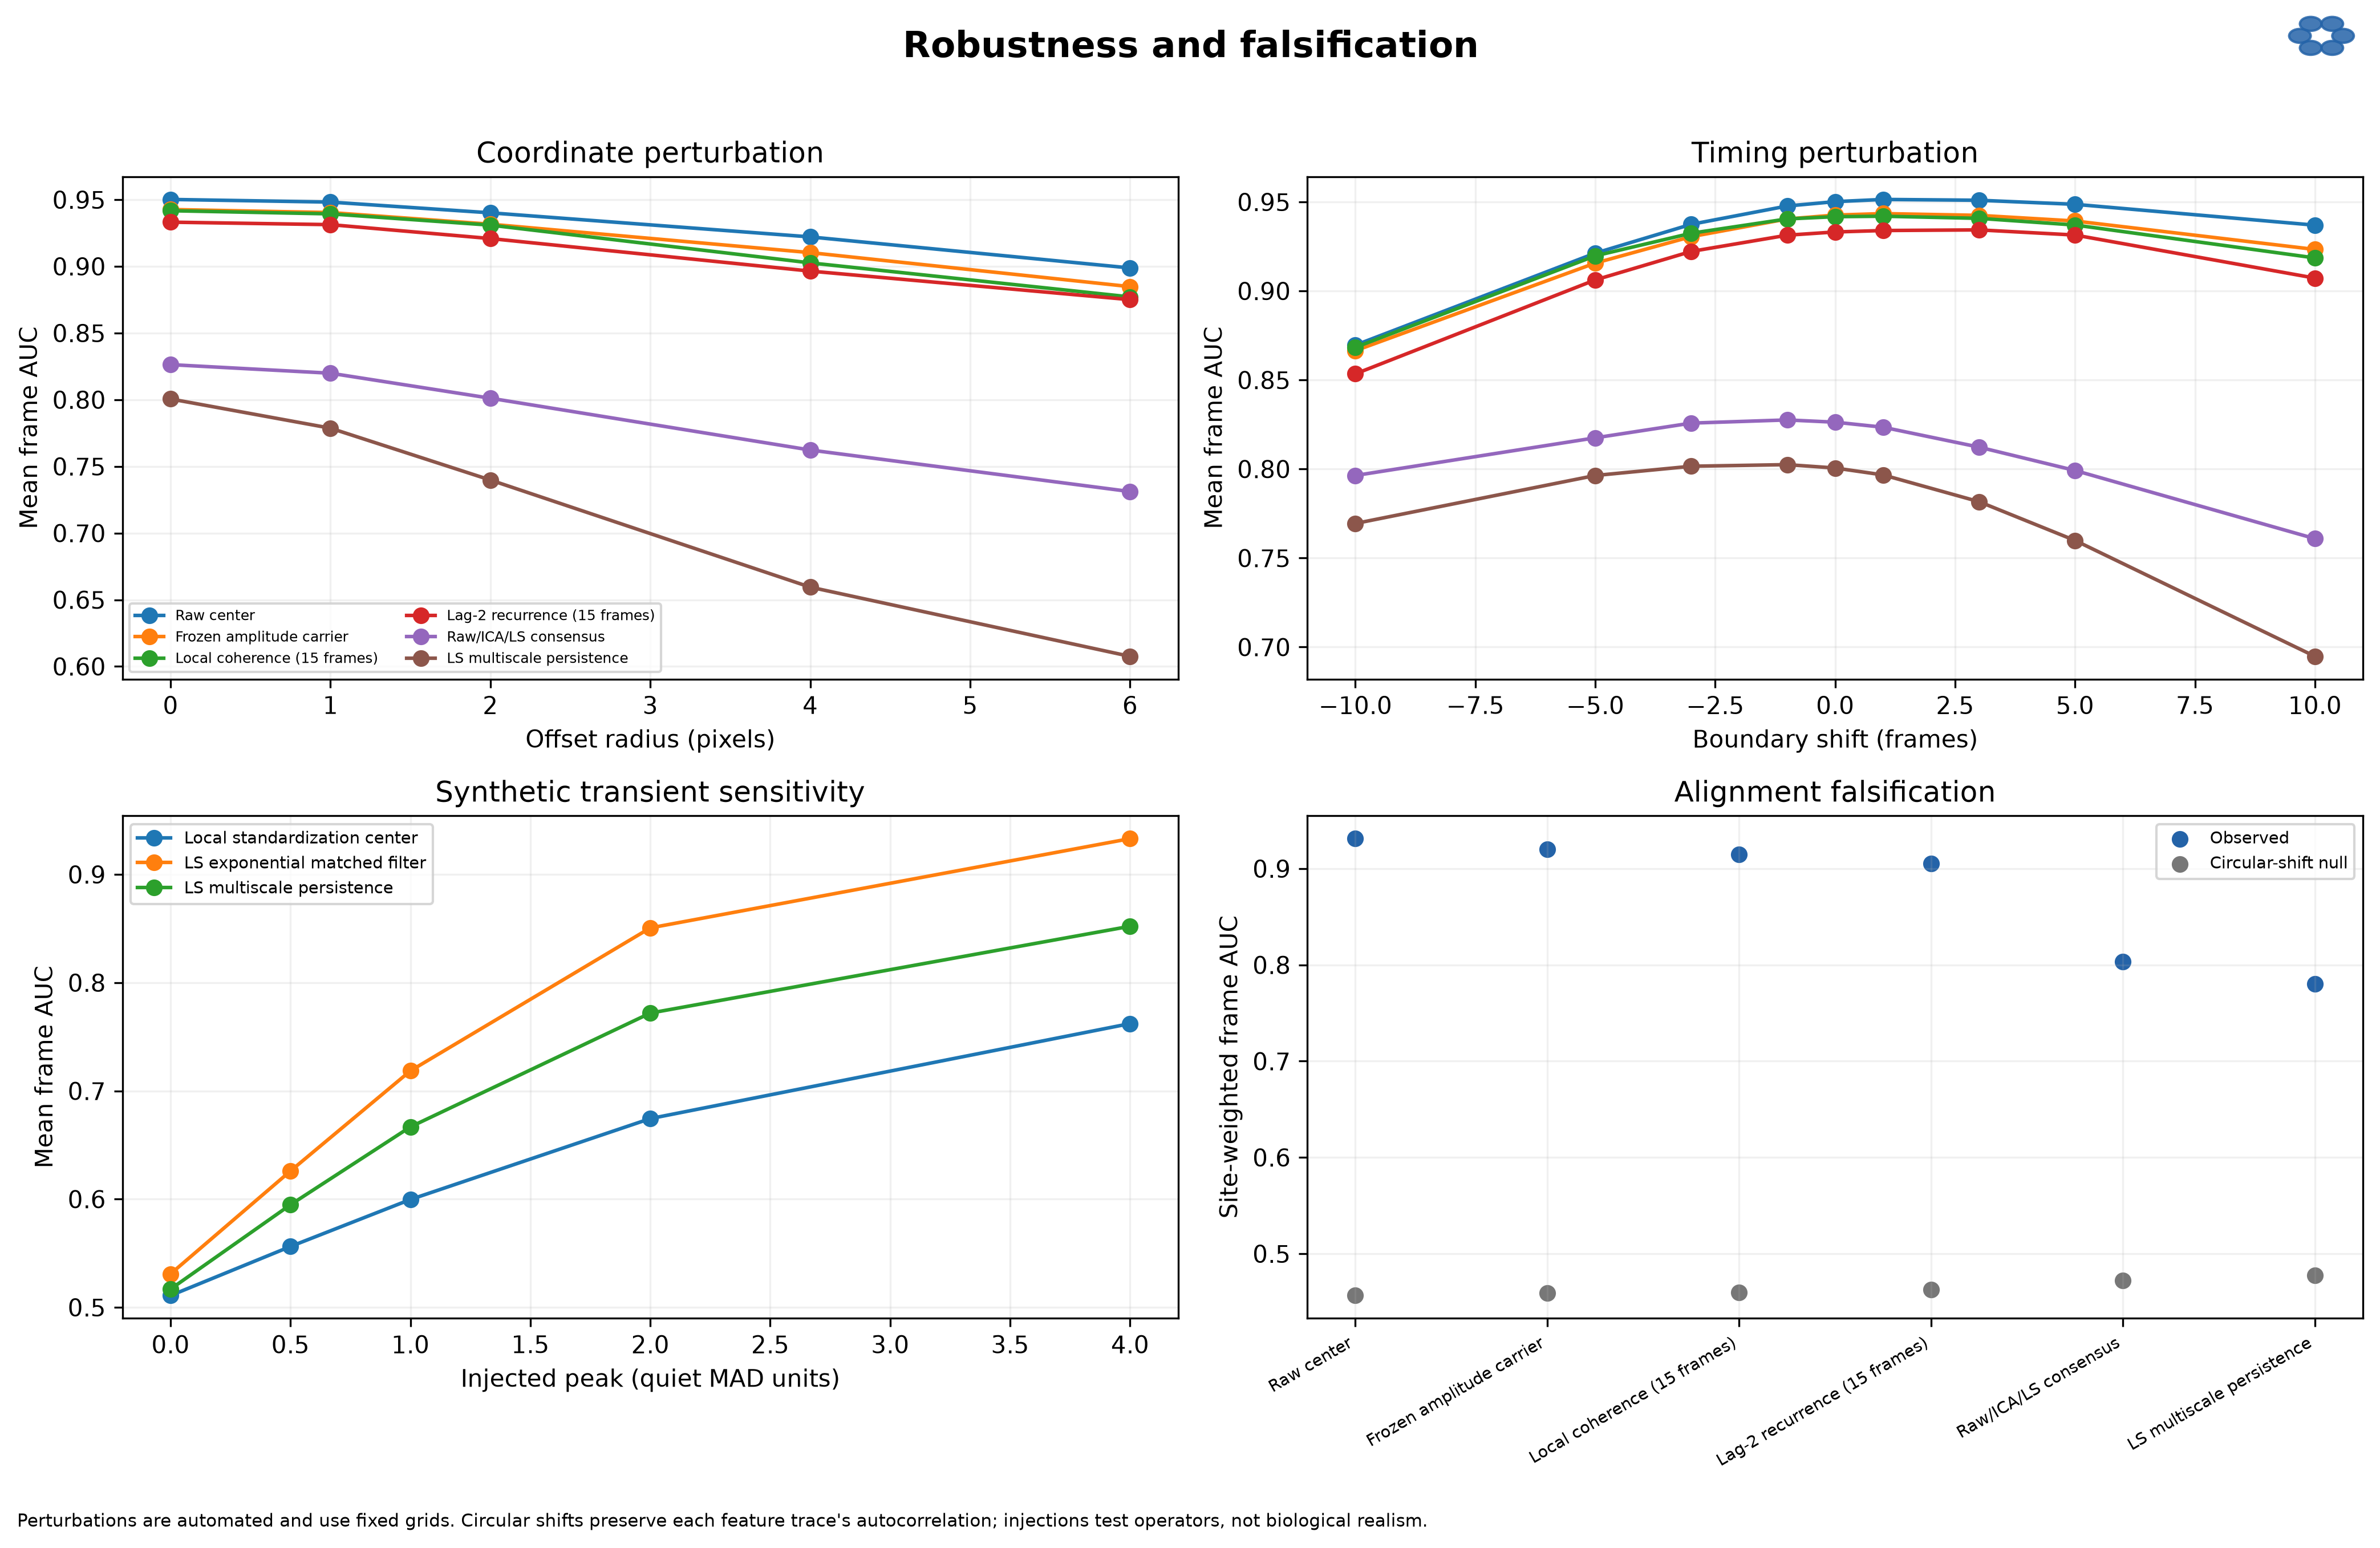
\includegraphics[width=0.98\linewidth]{figures/final/fig10_robustness_falsification.png}
  \caption{Fixed coordinate and timing perturbations, synthetic transient
  sensitivity, and site-blocked circular-shift falsification. The injection is
  one-dimensional and is not a biological or optical simulator.}
  \label{fig:robustness-falsification}
\end{figure}

\subsection{Deep dives separate proposal, ranking, kinetics, and failure modes}

At the frozen B58 operating point, \DeepRecoveredAll{} occurrences were
recovered by all three quantitative lanes, \DeepRecoveredPartial{} by a subset,
and \DeepAllMisses{} by none. Of the all-lane misses, five were uniform
localization misses and four were uniform identity conflicts; the remaining
three involved ranking, non-maximum suppression, or both. Recovered-minus-missed
center-AUC contrasts were positive for carrier, coherence, and lag, but every
site-bootstrap interval crossed zero.

The common-proposal analysis distinguished spatial proposal formation from
ranking on an identical candidate universe. At budget 20, coherence exceeded
carrier by \DeepCoherenceNativeTwenty{} recall in its native proposal stream but
only \DeepCoherenceRankingTwenty{} on common proposals. The corresponding lag-2
contrasts were \DeepLagNativeTwenty{} and \DeepLagRankingTwenty{}. These are
native-versus-common-proposal contrasts, not an additive causal decomposition,
but they indicate that the early-budget value is not explained by reranking
alone.

A fixed calcium-kinetic bank selected \DeepKineticKernel{} in every
leave-one-burst-out fold. Its overall site-weighted frame AUC was
\DeepKineticAUC{}, and the unweighted mean of held-burst AUCs was
\DeepKineticLOBOAUC{}. Across 20 repeated site-grouped splits, compact
carrier/coherence/lag recovery modeling changed log loss from
\DeepCarrierLoss{} to \DeepCompactLoss{}. The broader role-specific model was
stronger in point estimates, but only 12 all-lane misses make all recovery
models exploratory.

\subsection{Canonical-v8 review separates localization gain from identity reassignment}

The identity-aware review changed the interpretation of the 12 all-lane B58
misses without changing the canonical-v7 coordinates or labels. Under the fixed
six-pixel cross-stage consensus search, two response-maximizing candidates
collided with another geometry of the same canonical identity and six collided
with a different canonical identity. Only four candidates---ROI~19, ROI~22,
ROI~25, and ROI~27---were identity-clear within six pixels. Consequently, eight
of 12 apparent local improvements cannot be called coordinate corrections.

The reviewer-suggested ROI~23 shift approached ROI~26, while the ROI~12
consensus landed exactly on ROI-new-002 and the suggested shift lay 2.24 pixels
from it. ROI~10 and ROI~15 formed a same-canonical-identity cluster, and all
three ROI~11 occurrences shifted toward ROI-new-001. Among the identity-clear
cases, ROI~22 remained noise-dominated, ROI~19 was plausible but noise-limited,
ROI~27 retained a credible crowded-field transient consistent with
non-maximum-suppression failure, and ROI~25 remained a noisy ranking case. This
canonical-v8 result is a reviewed failure-interpretation update, not a revised
truth set or evidence of one-to-one biological source recovery.

The strict detector result therefore remains $94/106=88.7\%$, and the existing
canonical-collapsed sensitivity remains $93/102=91.2\%$
(\Cref{tab:identity-aware-v8}). Excluding the eight collision occurrences gives
an audit-conditioned $94/98=95.9\%$ sensitivity among currently
identity-resolved occurrences, but this is not an updated detector recall. Even
if all four identity-clear hypotheses were later validated and recovered, the
corresponding strict-recall ceiling would be $98/106=92.5\%$. Neither
sensitivity licenses counting an identity collision as a detection.

\begin{table}[!htbp]
\centering
\caption{Canonical-v8 identity-aware interpretation of the frozen B58 recovery
result. Only strict recall is an official detector metric. Audit-conditioned
and hypothetical values are sensitivities, not replacement performance
estimates.}
\label{tab:identity-aware-v8}
\small
\begin{tabularx}{\linewidth}{>{\raggedright\arraybackslash}p{0.31\linewidth} >{\raggedright\arraybackslash}p{0.20\linewidth} X}
\toprule
Quantity & Value & Interpretation \\
\midrule
Strict recovered occurrences & $94/106=88.7\%$ & Frozen official known-positive recall; unchanged by v8. \\
Canonical-collapsed sensitivity & $93/102=91.2\%$ & Existing duplicate-collapsed sensitivity; unchanged by v8. \\
All-lane misses & $12/106=11.3\%$ & Frozen miss count entering the identity-aware audit. \\
Same-identity collisions & $2/12=16.7\%$ & Candidate approaches another geometry assigned to the same canonical identity. \\
Different-identity collisions & $6/12=50.0\%$ & Candidate approaches a different labeled canonical identity. \\
Identity-clear hypotheses & $4/12=33.3\%$ & ROI 19, 22, 25, and 27 remain unresolved localization, noise, ranking, or NMS hypotheses. \\
Identity-resolved conditional sensitivity & $94/98=95.9\%$ & Descriptive sensitivity after excluding eight collision occurrences from the evaluable denominator; not official recall. \\
Four-case rescue ceiling & $98/106=92.5\%$ & Hypothetical strict recall if every identity-clear candidate were independently validated and recovered. \\
\bottomrule
\end{tabularx}
\end{table}


The automated identity-aware feature panel then tested cross-stage offset
stability, point/disk/footprint extraction, response-footprint morphology,
local competition, and neighboring-trace leakage without fitting a classifier
to the four identity-clear misses (\Cref{fig:identity-aware-features}). Median
pairwise offset-direction cosine was 0.972 for collision cases versus 0.448 for
identity-clear misses, while median offset-vector spread was 1.13 versus 1.83
pixels. This is consistent with a strong neighboring source pulling multiple
representations in the same direction; it is not evidence that the collision
coordinate belongs to the missed identity.

Local-standardized candidate traces also retained more neighboring-trace
structure in collision cases. Median candidate--neighbor partial correlation
after removing the original-center trace was 0.474 for collisions and 0.182
for identity-clear misses; median nonnegative neighbor weight was 0.460 versus
0.187. ROI~12 was the limiting example, with partial correlation and neighbor
weight both equal to 1.0 at the candidate that coincided with ROI-new-002.

Footprint morphology was not a strong separator: median eccentricity was 0.774
for collisions and 0.810 for identity-clear misses, with median solidity 0.781
and 0.714. Response-weighted extraction increased median local-standardized
event peak relative to pre-event MAD from 4.06 to 22.99 in collision cases and
from 3.97 to 12.67 in identity-clear misses. Because the footprint weights were
selected from the same event response, these gains establish extraction
sensitivity rather than prospective recovery or identity specificity.

Among identity-clear cases, ROI~19 had perfectly aligned stage offsets and low
neighbor leakage, making it the cleanest localization hypothesis despite weak
spatial support. ROI~25 also had consistent offsets and low leakage but an
irregular footprint. ROI~22 and ROI~27 had inconsistent stage offsets, favoring
noise or crowded-field instability over a stable point correction.

The broader frozen validation suite strengthened the proposal-absence
interpretation. No identity-clear miss had a frozen candidate within eight
pixels by budget 100 in any carrier, coherence, or lag lane. These cases are
therefore not merely B58 ranking failures in the audited candidate inventory.
Collision cases retained some nearby candidates because the inventory can
approach the competing identity. Leave-one-stage-out candidate gain was 1.54
for collisions and 1.31 for clear misses, but the exact occurrence-grain
permutation value was 0.371.

Multi-neighbor fits explained median 52.3\% of collision-candidate variance
versus 8.8\% for clear misses. After subtracting neighboring traces, median
event peak/MAD was 4.02 versus 5.48. Pre-event-frozen footprints retained
median peak/MAD 11.98 and 9.51, respectively, demonstrating prospective
within-recording extraction sensitivity without target-event footprint
selection. Recovered-site response maximization shifted a median 2.24 pixels,
while quiet pseudo-events shifted 5 pixels, confirming that unconstrained
recentring itself creates displacement. Cross-burst transfer produced 34
collision source--target pairs but only one clear pair and therefore could not
compare the groups. None of three exact eight-versus-four descriptive tests
was small ($p=0.371$, 0.169, and 0.308).

\subsection{Expanded automated tests prioritize observability context and abstention}

Ten additional frozen test families evaluated identity-grouped prediction,
site-bootstrap stability, conditional importance, prospective transfer,
controlled mixtures, metamorphic behavior, selective risk, recovered-only
anomaly detection, and graph crowding (\Cref{fig:expanded-automated-v3}). The
full panel reached identity-grouped ROC AUC 0.833 and log loss 0.498, compared
with AUC 0.611 and log loss 0.690 for carrier alone. These values strengthen
within-recording error stratification rather than establish generalization.

Across 100 site-bootstrap sparse fits, variance-stabilized center-annulus was
selected in 97\%, multiscale persistence in 73\%, lag-2 recurrence in 39\%, and
the matched filter in 29\%. Within-burst conditional permutation increased log
loss by 0.0484, 0.0244, and 0.0234 for the first three features. The annular
result is not necessarily neural: its weak event retrieval and high stability
indicate persistent observability, background, or acquisition context.

Confidence-based abstention reduced internal error from 20.8\% at full coverage
to 9.4\% at 50\% coverage. Recovered-only isolation-forest and robust-distance
scores separated misses with AUC 0.814 and 0.760. A simple five-neighbor graph
statistic had negligible association with recovery ($r=-0.009$), showing that
distance-only crowding is inadequate. Controlled mixtures and metamorphic
checks behaved directionally: neighboring transients could inflate peak/MAD,
common mode reduced event contrast while increasing lag recurrence, frozen
intensity scaling preserved peak/MAD, and temporal shifts changed fixed-window
retrieval. These one-dimensional checks validate operators, not movie
formation.

\begin{figure}[p]
  \centering
  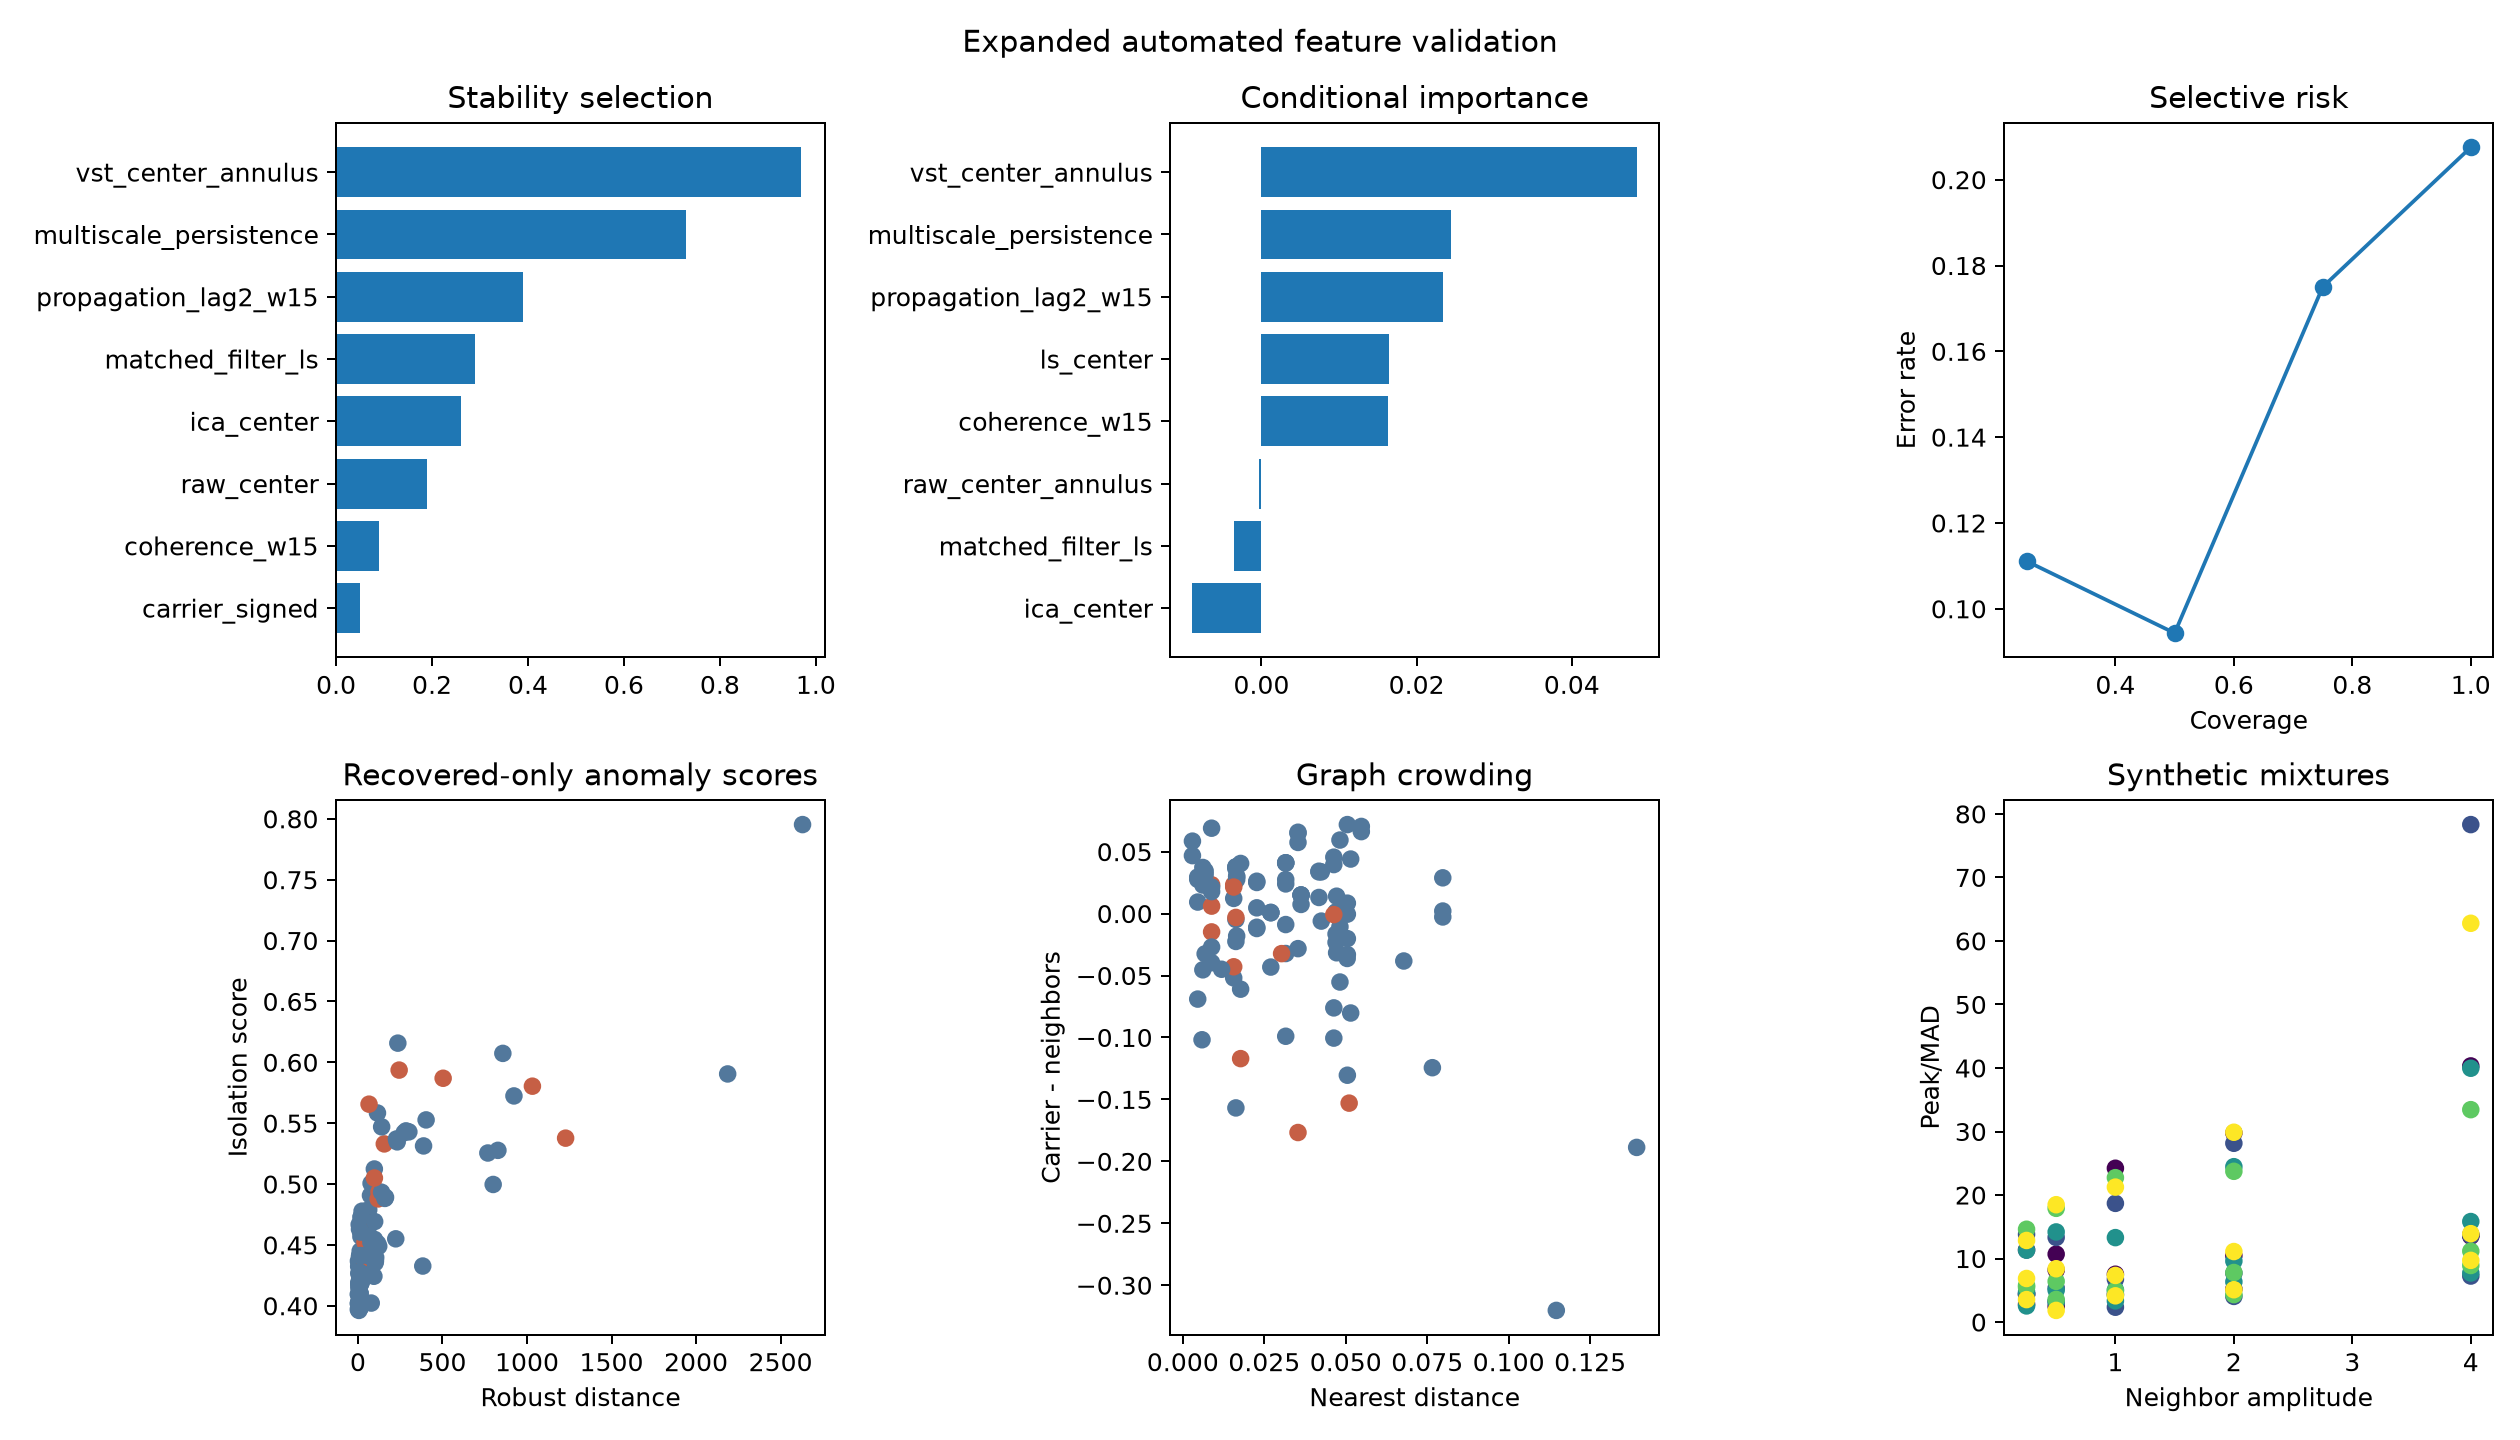
\includegraphics[width=0.99\linewidth]{figures/final/fig14_expanded_automated_validation.png}
  \caption{Expanded automated validation. Stability, importance, selective
  risk, anomaly, graph, and synthetic panels are exploratory within one
  recording; unmatched candidates remain unknown and synthetic mixtures are
  one-dimensional.}
  \label{fig:expanded-automated-v3}
\end{figure}

\begin{figure}[p]
  \centering
  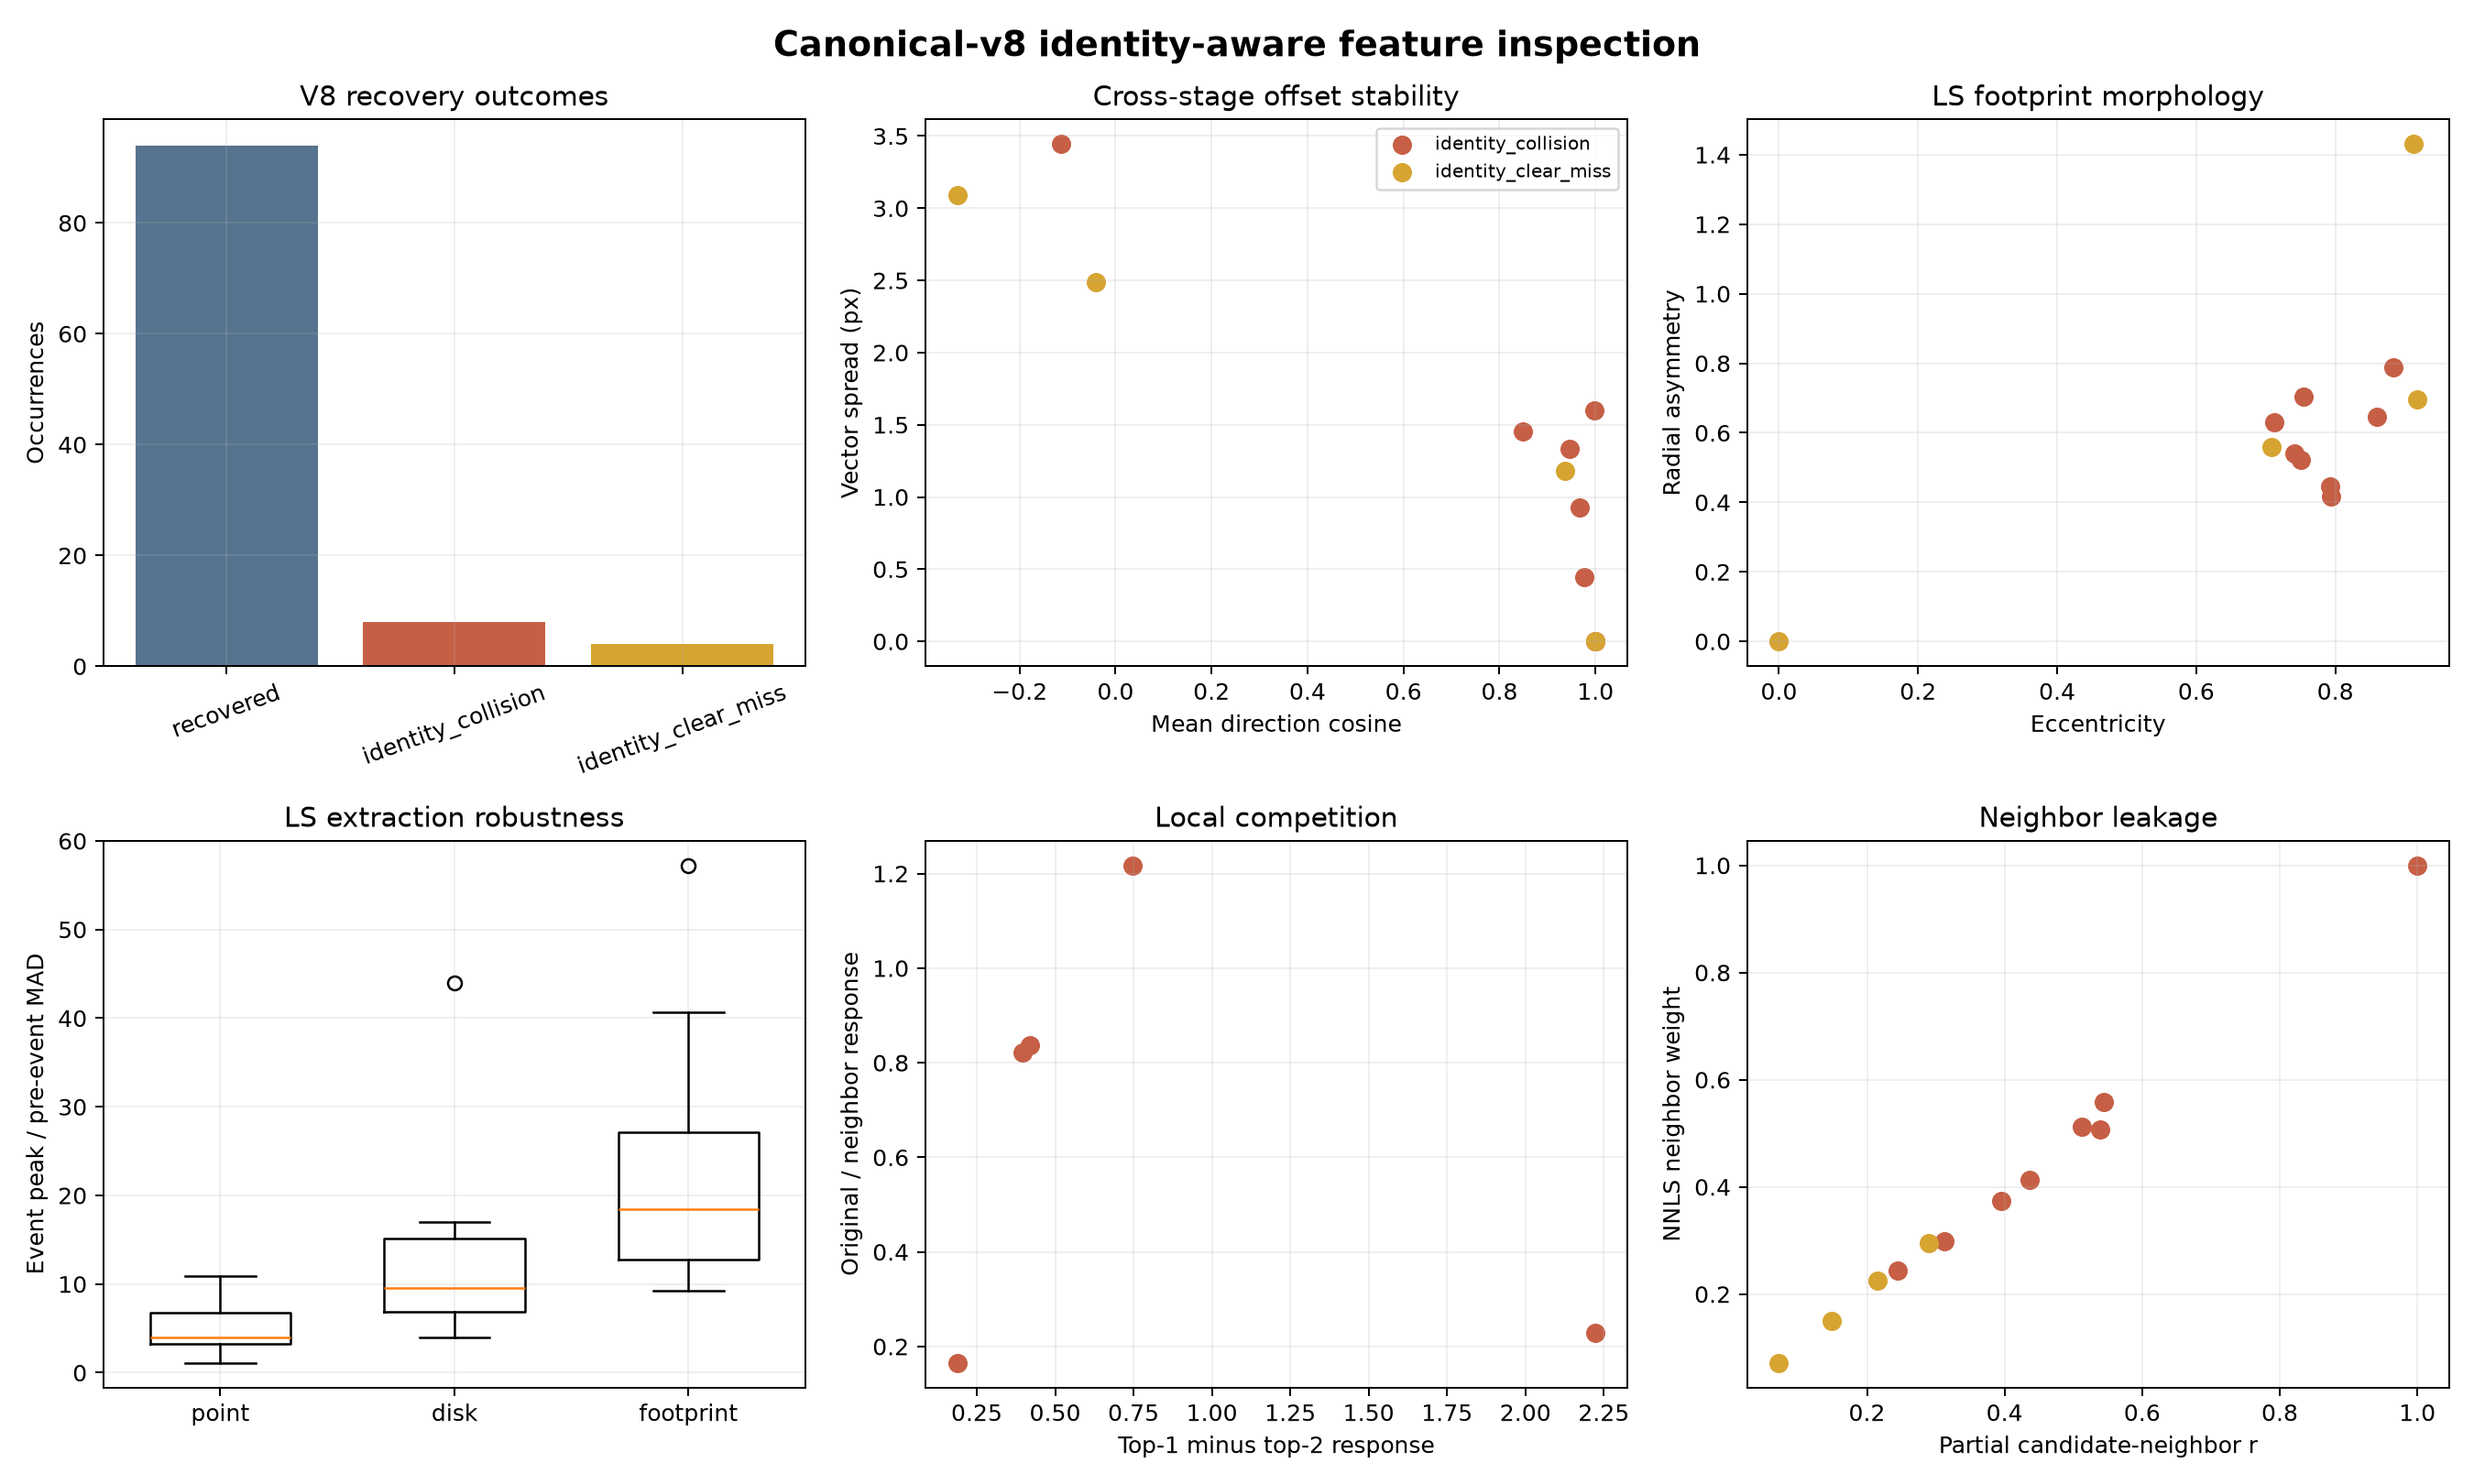
\includegraphics[width=0.99\linewidth]{figures/final/fig13_identity_aware_feature_inspection_v8.png}
  \caption{Canonical-v8 identity-aware feature inspection. The three-outcome
  panel is descriptive; collision and identity-clear groups contain eight and
  four misses. Footprint extraction is response-selected from the same events,
  and nearest labeled geometry is not exhaustive biological truth.}
  \label{fig:identity-aware-features}
\end{figure}

\begin{figure}[p]
  \centering
  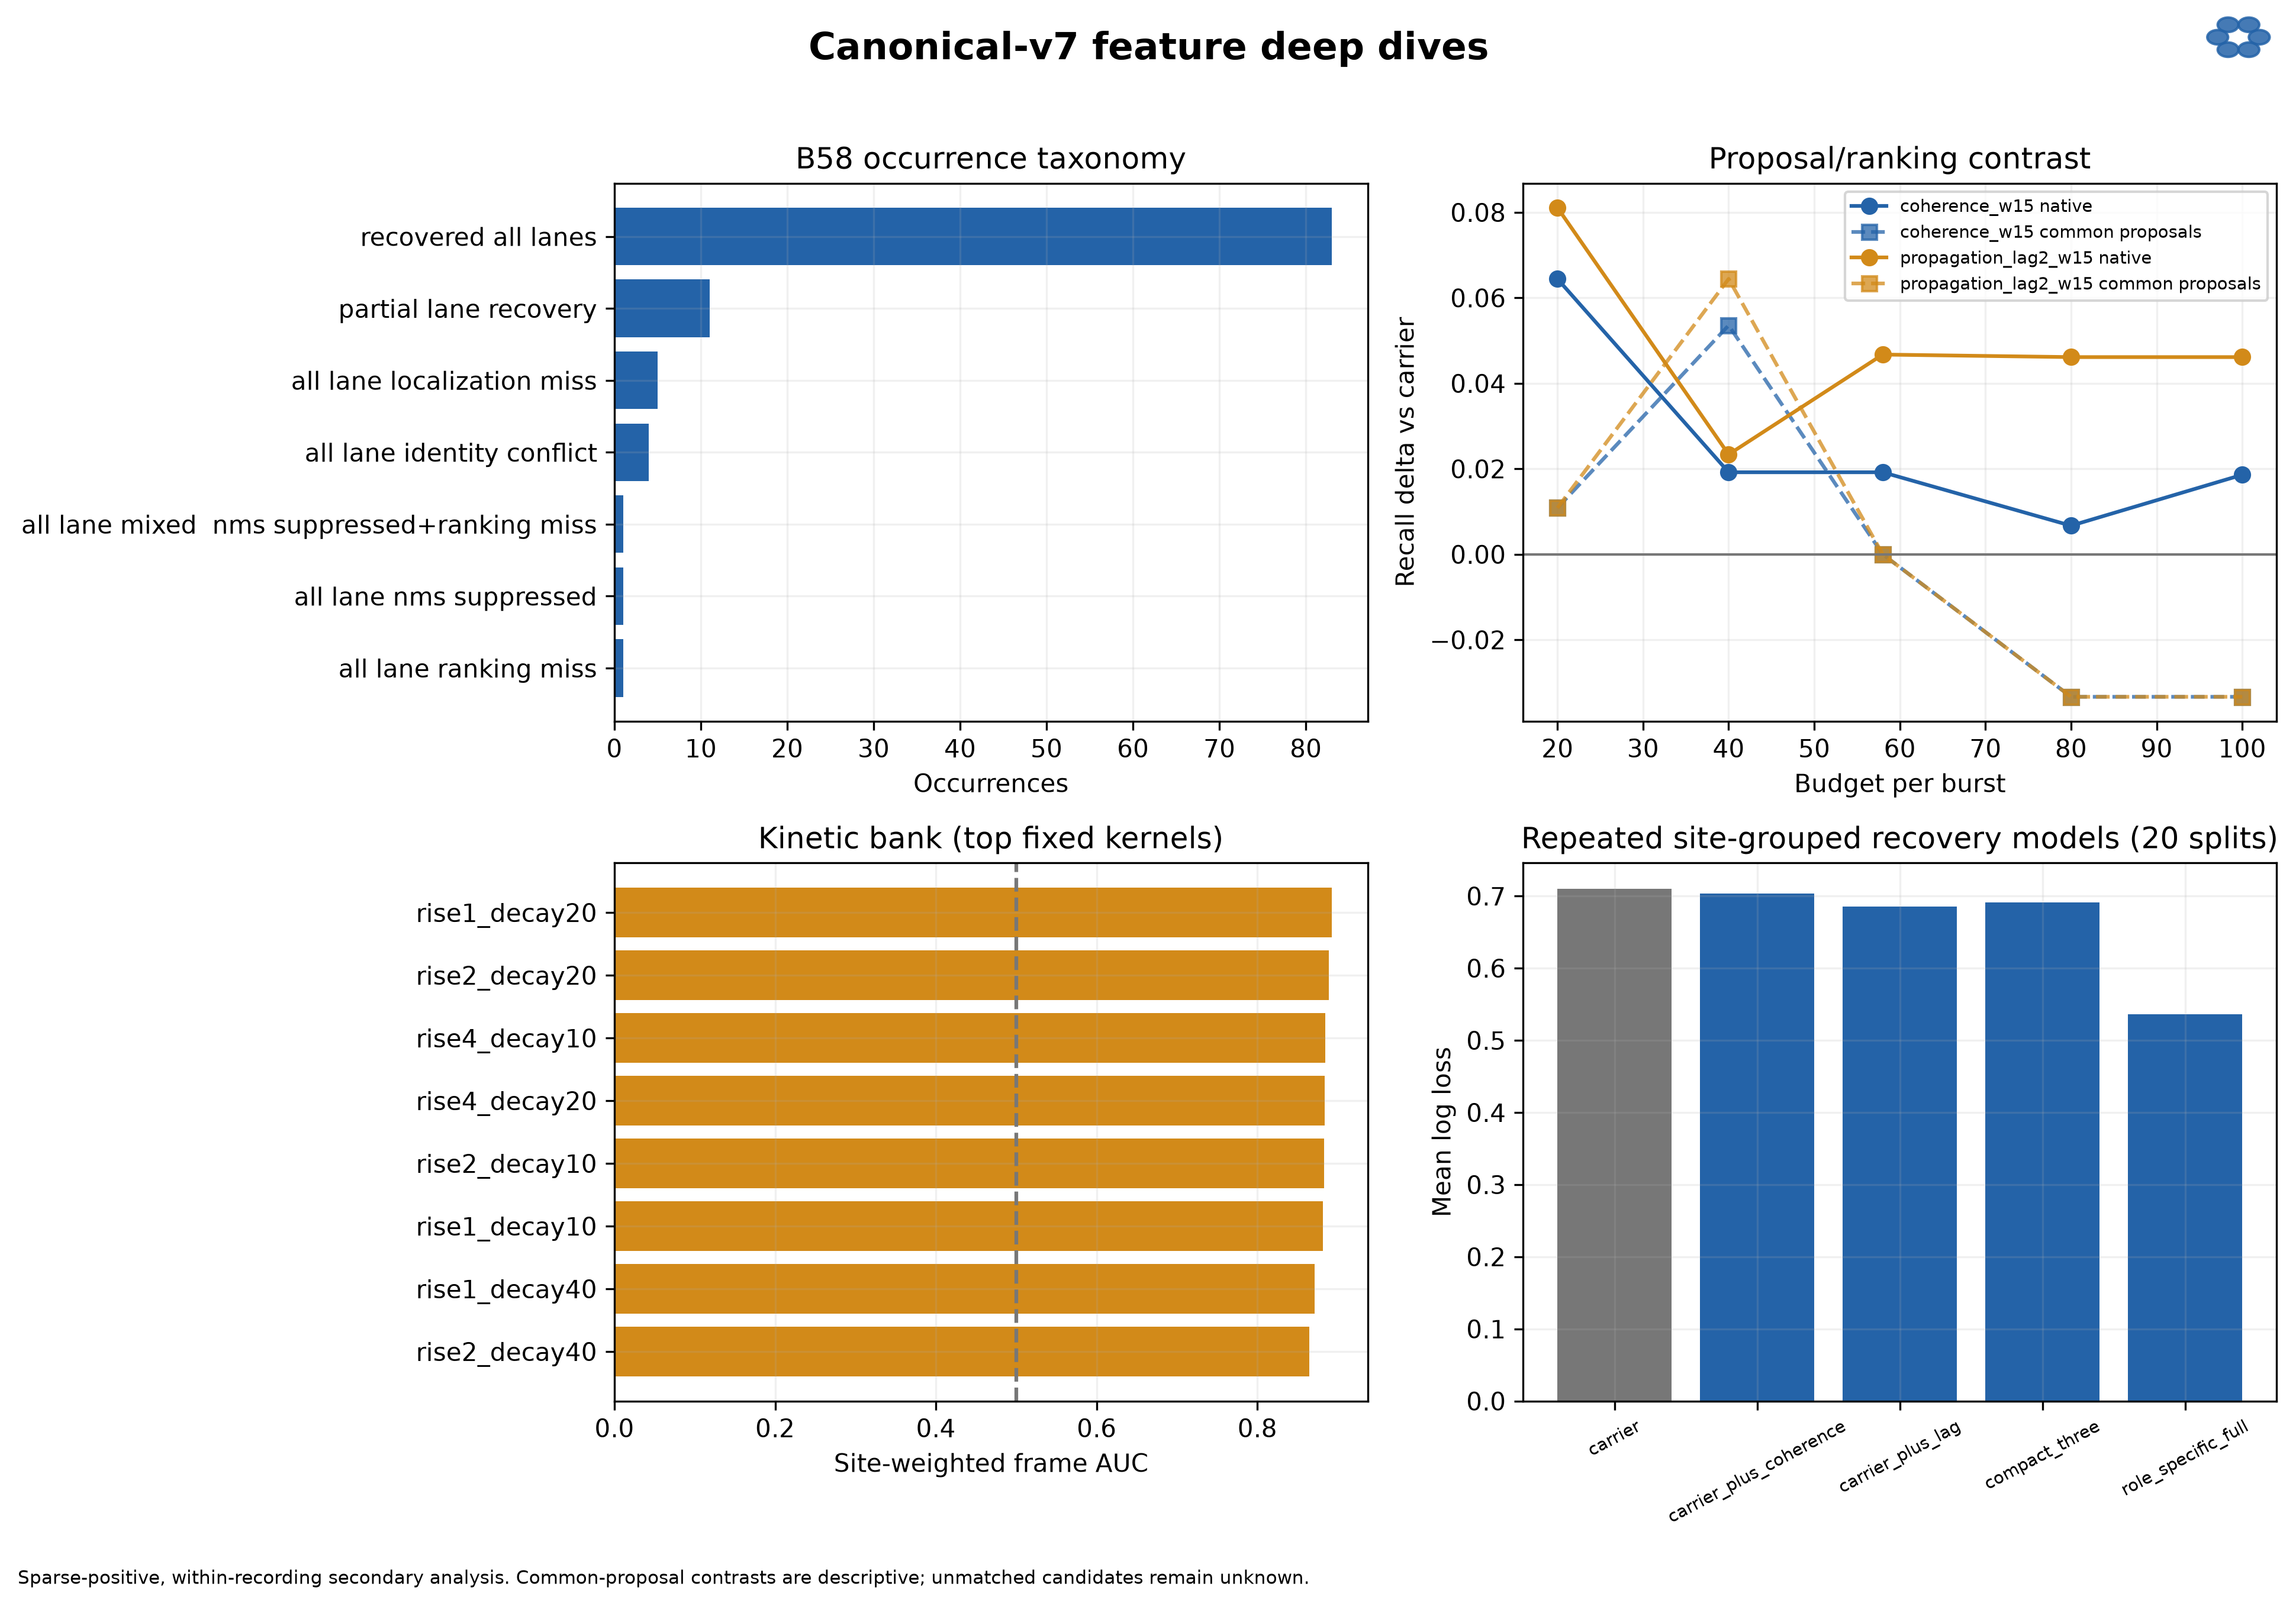
\includegraphics[width=0.98\linewidth]{figures/final/fig11_feature_deep_dives.png}
  \caption{Prespecified feature deep dives: exact B58 failure taxonomy,
  native-versus-common-proposal contrasts, a fixed kinetic filter bank, and
  repeated site-grouped recovery models. Sparse positives and small failure
  counts limit interpretation.}
  \label{fig:feature-deep-dives}
\end{figure}

\begin{figure}[!htbp]
  \centering
  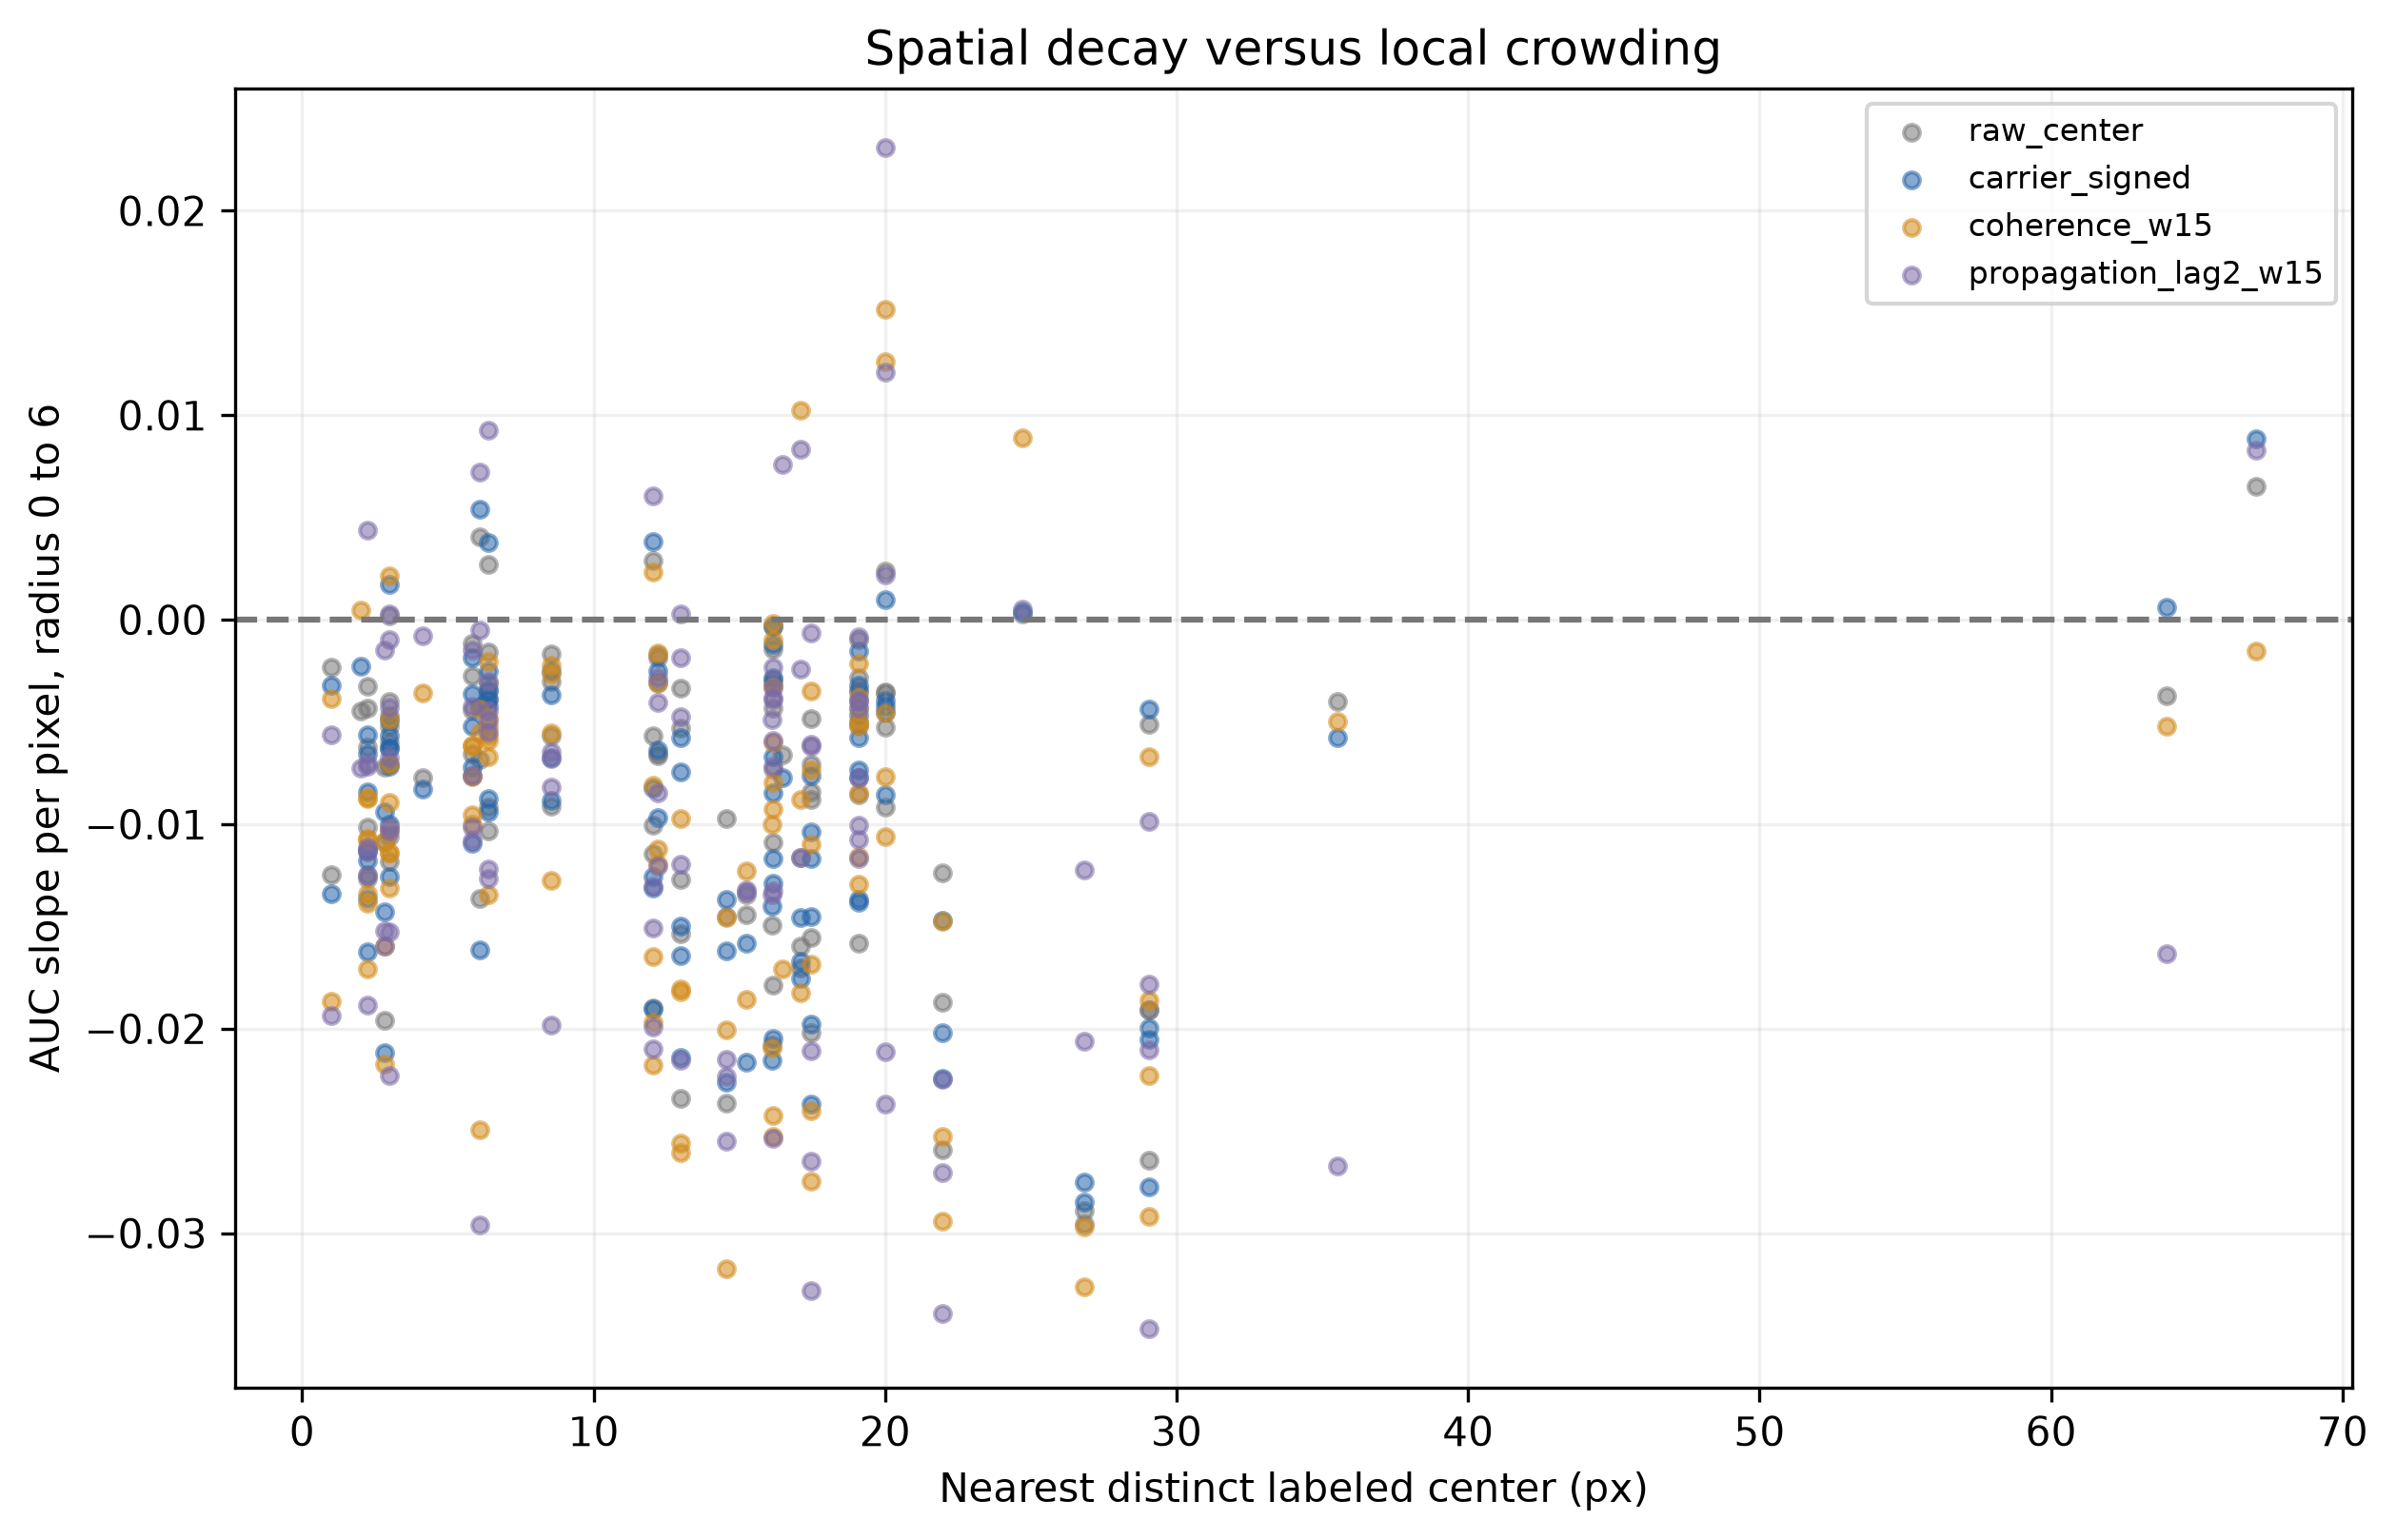
\includegraphics[width=0.86\linewidth]{figures/final/fig12_spatial_decay_crowding.png}
  \caption{Radius-0-to-6 retrieval decay versus the nearest distinct labeled
  center. Duplicate burst occurrences at one immutable site are not counted as
  spatial neighbors; labeled-center density is an incomplete crowding proxy.}
  \label{fig:spatial-decay-crowding}
\end{figure}

\DraftFigure{Recall-versus-candidate-budget curves for the frozen representation panel, proposal-union ceilings, same-proposal ranking comparisons, and failure categories. A separate panel will report bounded-field precision--recall after blinded exhaustive review.}{Detection implications under positive--unlabeled annotation.}{fig:detection-implications}

\subsection{Acquisition structure is a potential determinant of observability}

Preliminary quiet-frame analysis reported an intensity--variance slope of approximately \QuietVarianceSlope{} with weighted $R^2$ between \QuietVarianceWeightedRtwo{}. The audit also identified a provisional field boundary near \ProvisionalFieldBoundaryX{} and a left--right global-trace correlation of \LeftRightGlobalCorrelation{}. These observations motivate stratification by field, saturation, baseline intensity, motion, and local effective rank. The final analysis will determine whether recurrently difficult sites are explained by biological event magnitude, acquisition position, local contamination, or a combination of these factors.

\DraftFigure{Variance-versus-intensity fit, saturation and motion maps, field-boundary diagnostics, temporal spectra, and a comparison of the canonical recording with any available unlabeled recordings.}{Acquisition physics and recording-quality context.}{fig:acquisition-qc}

\subsection{Detection occurrences form recurring measurement-profile classes}

The maximum-filter audit revealed that flat feature-map plateaus could contribute adjacent pixels to a nominal non-maximum-suppressed candidate list. We therefore repeated the frozen analysis with explicit Euclidean object separation and a label-free event-maximum tie breaker. Both compact lanes retained their positive known-positive-recall gains across the prespecified 4, 6, and 8 pixel sensitivity settings. At the primary 6 pixel, budget-20 operating point, the cross-lane union contained 86 distinct detection occurrences at 36 consolidated spatial detection sites.

We constructed an 11-variable profile for every detection occurrence using native and residual peak amplitude, robust signal-to-noise ratio, spatial specificity, annulus coupling, signed event area, relative peak time, lane agreement, candidate rank, cross-burst recurrence, and quiet intensity. Continuous measurement features were robustly standardized within burst so that clustering would not merely reproduce burst intensity. Expert labels were excluded from fitting. Candidate solutions with two through six classes were compared using silhouette separation and bootstrap adjusted Rand stability, with a minimum of five occurrences and two bursts per class. The selected three-class solution had silhouette 0.284 and mean bootstrap adjusted Rand index 0.724; every class occurred in all four bursts.

\begin{table}[!htbp]
\centering
\caption{Frozen label-free detection-profile classes. Medians are reported in native intensity units where applicable. Known-positive overlap is descriptive only and is not precision.}
\label{tab:detection-profile-classes}
\small
\begin{tabular}{p{0.29\linewidth}rrrrr}
\toprule
Class & Occurrences & Sites & Raw peak & Residual peak & Spatial specificity \\
\midrule
Localized, high-signal, recurrent & 35 & 12 & 618.7 & 280.4 & 0.319 \\
Broad, low-signal, early/episodic & 8 & 6 & 269.5 & 94.0 & 0.170 \\
Broad, lower-signal, recurrent & 43 & 24 & 271.6 & 97.2 & 0.192 \\
\bottomrule
\end{tabular}
\end{table}


\begin{figure}[!htbp]
  \centering
  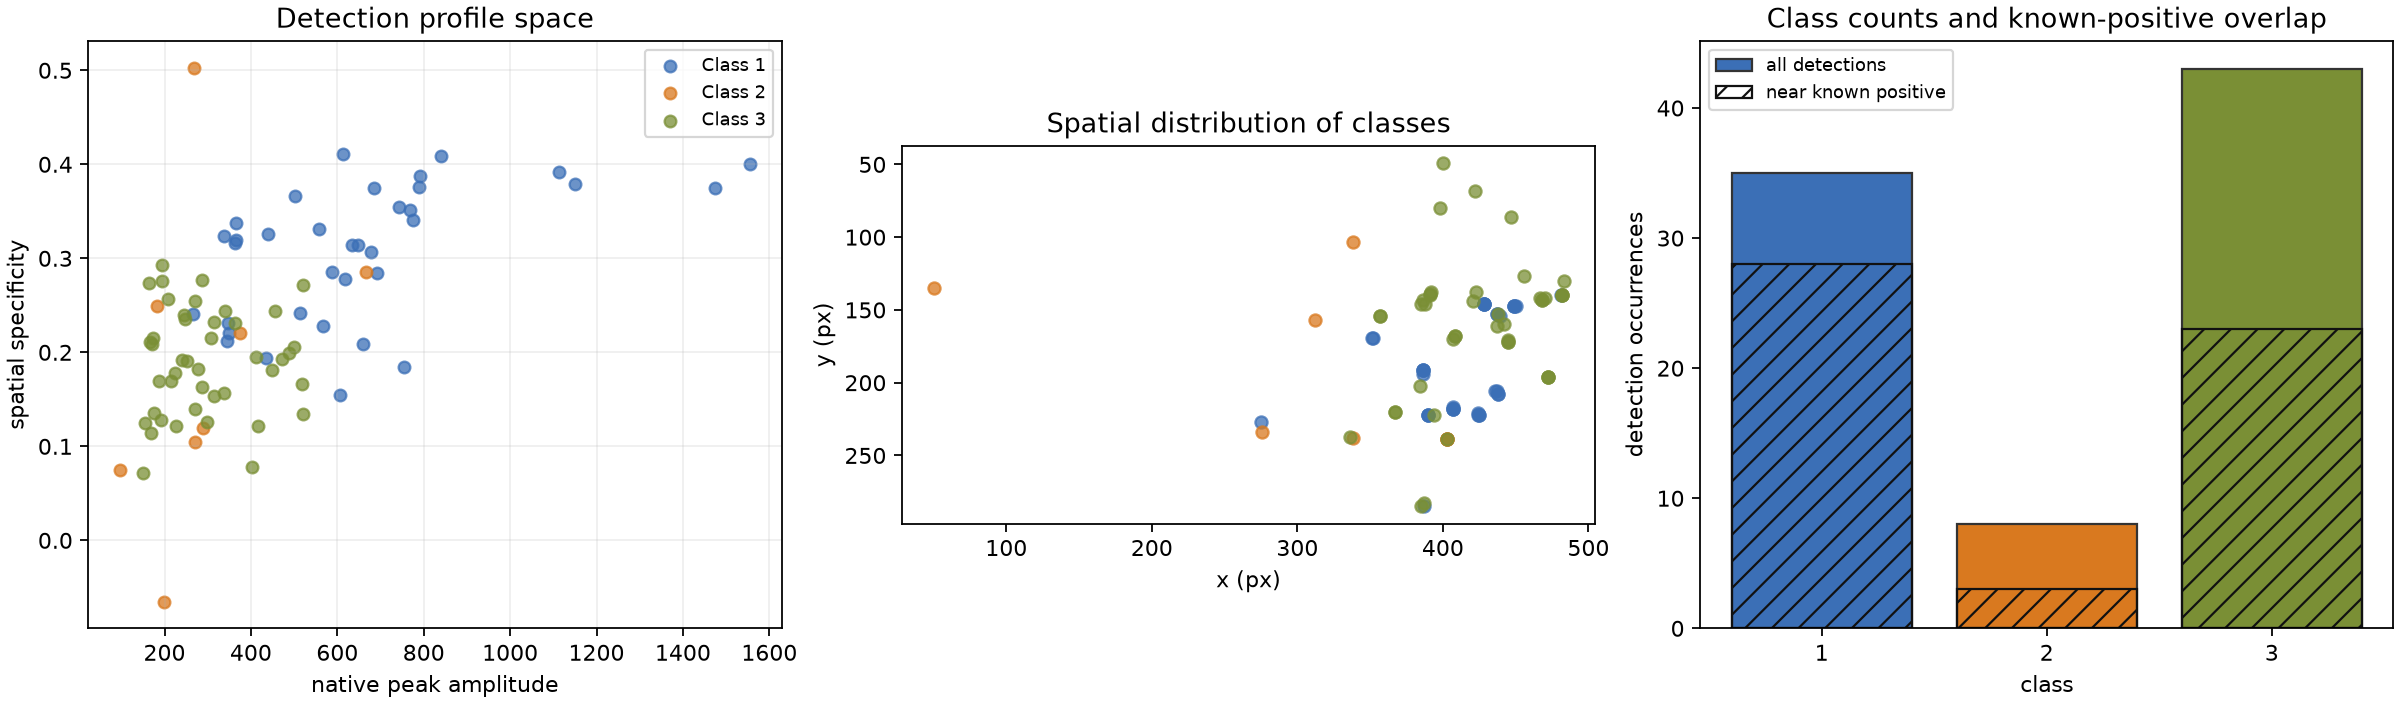
\includegraphics[width=0.98\linewidth]{figures/final/detection_class_overview.png}
  \caption{Label-free detection-profile taxonomy. Points are distinct strict-NMS detection occurrences. Class fitting did not use expert labels; hatched counts show post-freeze proximity to a sparse known-positive annotation and must not be interpreted as precision.}
  \label{fig:detection-profile-overview}
\end{figure}

\begin{figure}[!htbp]
  \centering
  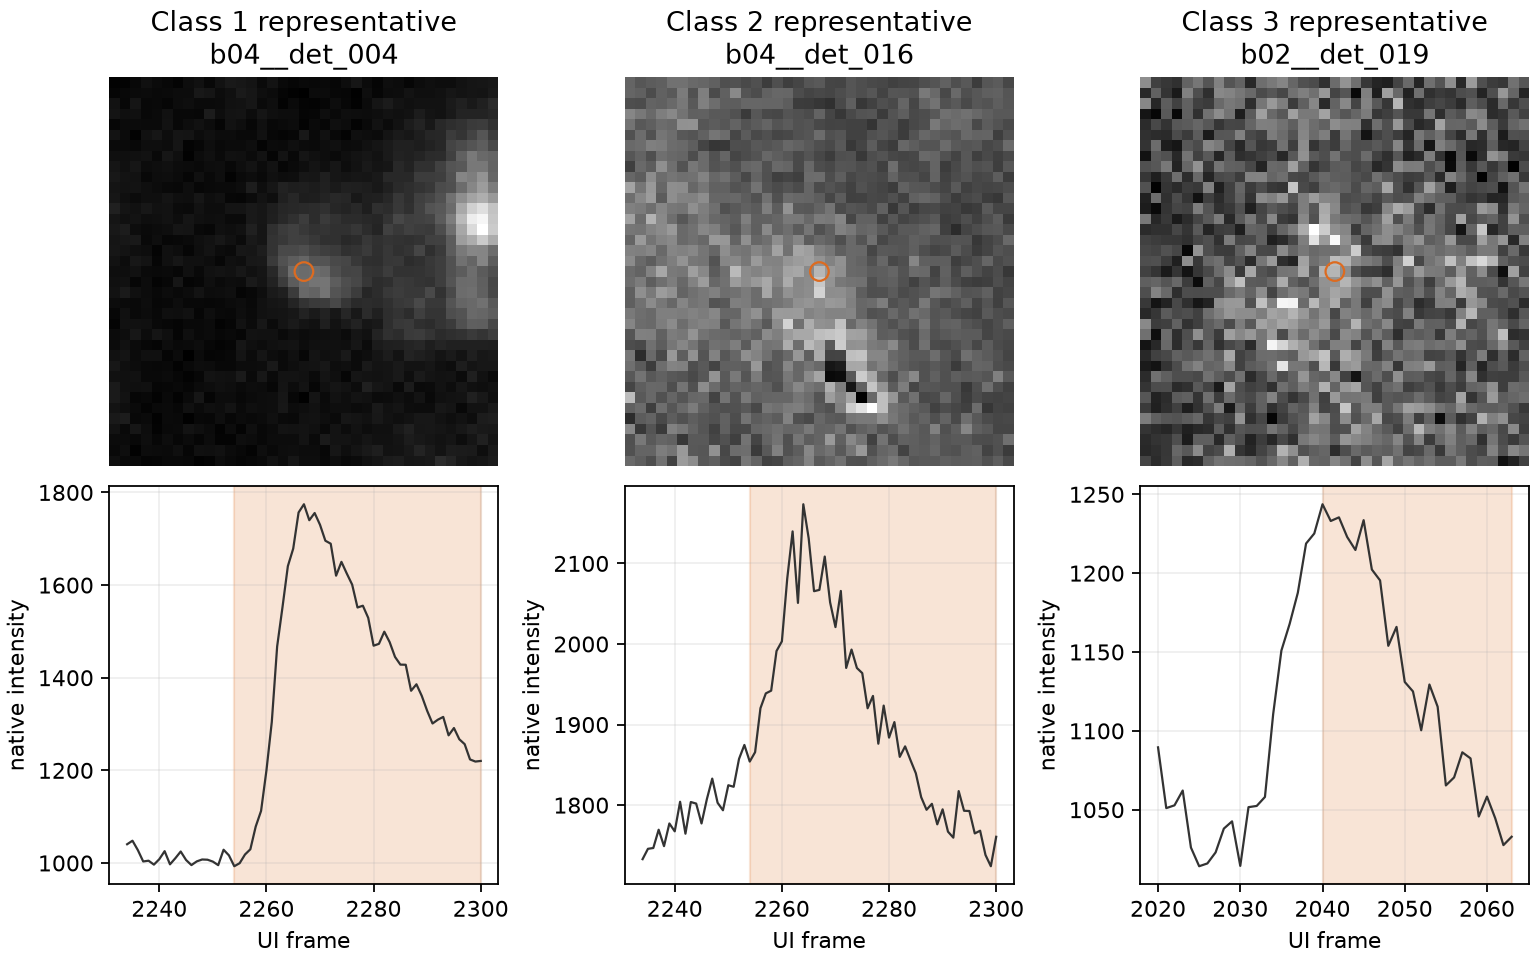
\includegraphics[width=0.98\linewidth]{figures/final/detection_class_representatives.png}
  \caption{Representative occurrence nearest each frozen class centroid. The top row shows event-maximum minus pre-event baseline crops; the bottom row shows native exact-site traces with the evaluated burst interval shaded. Classes describe measurement events, not biological cell types.}
  \label{fig:detection-profile-representatives}
\end{figure}

The largest localized, high-signal class contained 35 occurrences and showed the greatest overlap with sparse known positives (28 occurrences). The broad, low-signal early-peaking class contained eight occurrences, and the broad, lower-signal recurrent class contained 43. These overlap counts characterize already frozen classes; unmatched detections remain unknown rather than negative. The result supports discussion of recurring detection-event archetypes while preserving the positive--unlabeled boundary.

We next joined the frozen classes to adjudicated identity certainty without refitting or renaming the classes. In the frozen-v1 adjudicated subset, the strict budget-20 union matched 10 of 19 confirmed observations but none of five identity-uncertain observations (two-sided Fisher exact $p=0.053$); the single probable observation was retained as a separate category. This small subset suggests a possible observability gradient but is insufficient for a stable class-composition comparison. In expanded canonical v7, the union matched 34 of 54 confirmed and 10 of 22 identity-uncertain observations (Fisher exact $p=0.203$). Thus the expanded data do not establish a difference in overall detection coverage by certainty.

At the occurrence grain, confirmed observations contributed 8, 2, and 24 matches to Classes 1--3, whereas identity-uncertain observations contributed 0, 4, and 6. Because observations recur within identities, this table is descriptive only. The canonical-identity analysis below supersedes the earlier occurrence-level permutation result for inferential reporting.

Class membership was also longitudinally coherent. Among 50 ordered within-site transitions from 22 multiply detected sites, 42 (84\%) remained in the same class. Class 1 remained Class 1 in 22 of 24 transitions, Class 2 in 2 of 2, and Class 3 in 18 of 24. These results support treating the classes as recurring measurement regimes, while the observed transitions caution against assigning an immutable biological type to a spatial site.

\begin{figure}[!htbp]
  \centering
  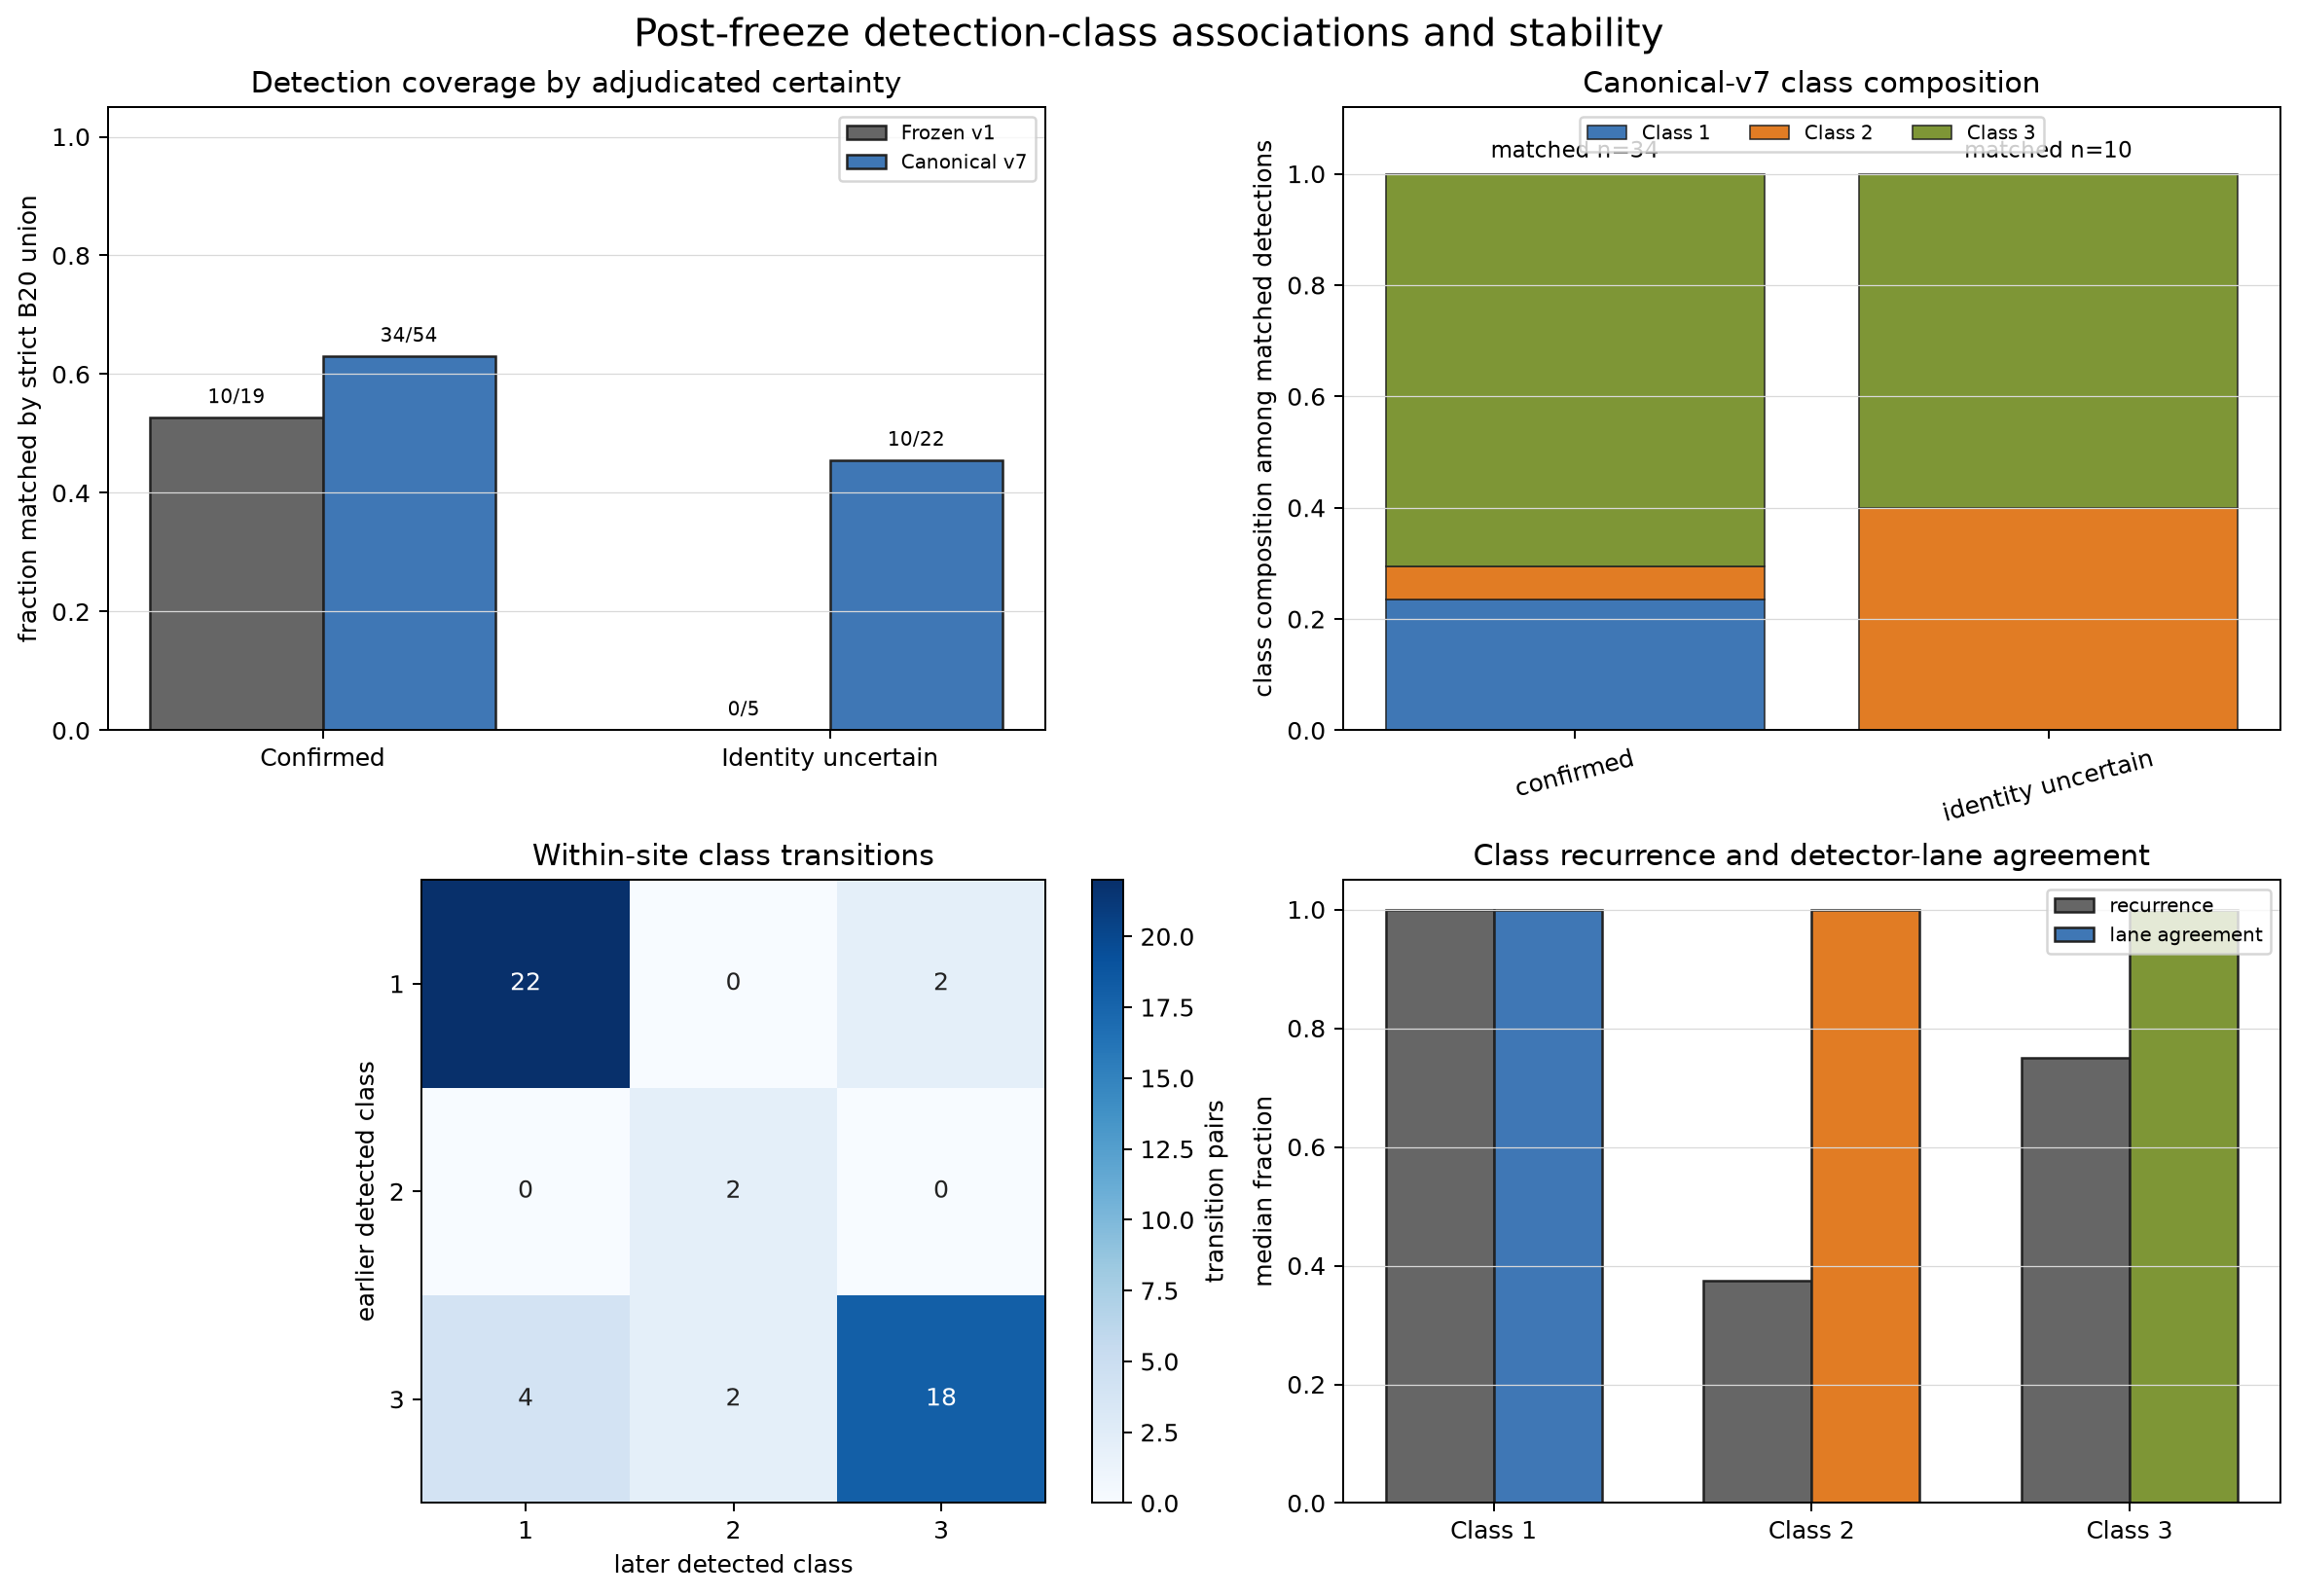
\includegraphics[width=0.98\linewidth]{figures/final/detection_class_extensions.png}
  \caption{Post-freeze class extensions. Detection coverage is reported against adjudicated certainty for frozen v1 and candidate-assisted canonical v7; class composition is shown only where both confirmed and identity-uncertain matched observations are available. The transition matrix follows repeated detection sites across ordered bursts. All associations are descriptive and do not redefine the frozen classes.}
  \label{fig:detection-class-extensions}
\end{figure}

Further post-freeze profiling separated reviewer uncertainty from clustering ambiguity. We defined a relative centroid margin from the nearest and second-nearest frozen class centers; this is a geometric separation measure, not a calibrated probability. Median margins were 0.511, 0.440, and 0.474 for Classes 1--3. Confirmed and identity-uncertain canonical-v7 matches had similar margins (0.473 versus 0.511; Mann--Whitney $p=0.790$). Thus uncertain identity was not explained by detections simply lying near a class boundary.

Reviewer morphology provided a more direct association. Among 45 matched adjudicated canonical-v7 observations, localized-boundary morphology contributed 8, 3, and 27 observations to Classes 1--3, whereas ambiguous or non-neuronal boundary morphology contributed 0, 4, and 3 ($V=0.503$). Challenging or structured contexts contributed 0, 5, and 5 observations, isolated contexts 8, 2, and 20, and overlapping contexts 0, 0, and 5 ($V=0.411$). These candidate-assisted associations reinforce the interpretation of Class 1 as spatially localized and Class 2 as a broad or difficult measurement regime, but they are not independent class validation.

Spatial effects were evaluated at the 36-site consolidated grain to avoid counting recurrent sites repeatedly. Relative to the provisional $x=286$ field boundary, the left/right site counts were 1/9 for Class 1, 2/4 for Class 2, and 0/20 for Class 3. The post hoc site-label permutation value was $p=0.041$ ($V=0.433$). Because only three sites lay left of the boundary and the boundary remains provisional, this result motivates acquisition-field stratification rather than an anatomical class claim. Conversely, burst composition showed little evidence of drift ($V=0.178$, permutation $p=0.503$), consistent with the classes recurring across all four events.

Canonical-v7 matching produced 24 identity trajectories, eight with detections in at least two bursts. The median dominant-class fraction among these multi-burst identities was 1.0, while specific identities such as ROI~014 and ROI-new-002 changed class in one burst. These cases provide a bounded review queue for distinguishing true measurement-regime changes from registration, overlap, or event-amplitude effects.

\subsection{Spatial ICA is localized at labeled coordinates but not temporally persistent}
\label{sec:spatial-ica-results}

Relative to matched translated controls, spatial-ICA event maps had greater center--annulus contrast (mean site-blocked difference \SpatialICAContrastDelta{}, $q=\SpatialICAContrastQ{}$), smaller effective radius (\SpatialICARadiusDelta{} pixels, $q=\SpatialICARadiusQ{}$), and smaller peak offset (\SpatialICAPeakOffsetDelta{} pixels, $q=\SpatialICAPeakOffsetQ{}$). Boundary sharpness was also greater after correction. Compactness and temporal persistence were not supported for spatial ICA. Raw maps showed the same directional localization pattern, with the exception that Raw compactness also differed. These comparisons establish representation-internal localization at protected coordinates, not neuronal identity and not precision against biological negatives.

\begin{figure}[!htbp]
  \centering
  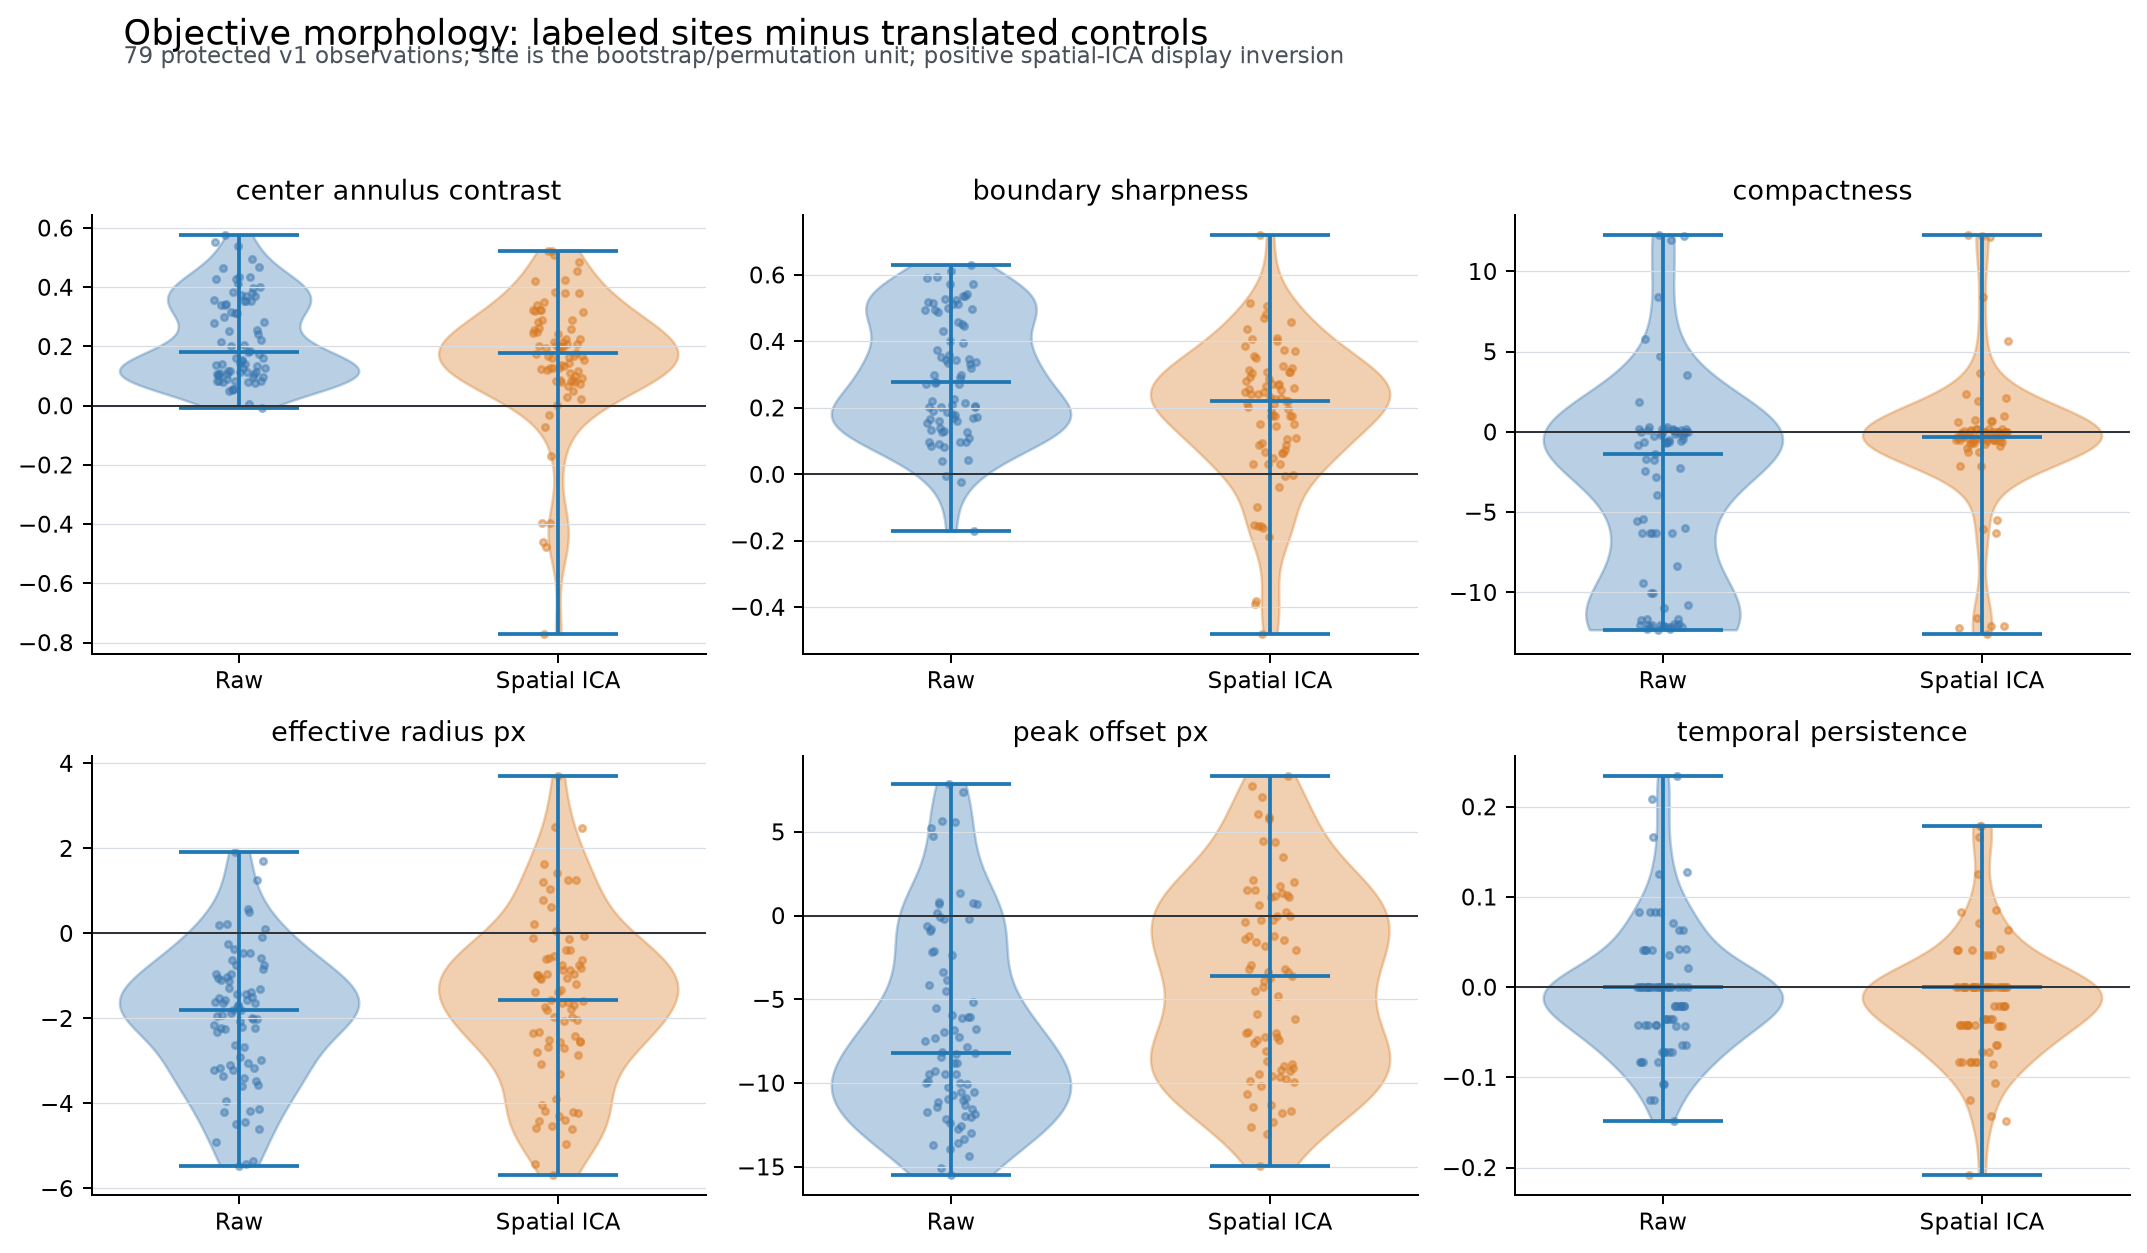
\includegraphics[width=0.98\linewidth]{figures/final/spatial_ica_objective_morphology.png}
  \caption{Objective morphology at protected-v1 coordinates and deterministic translated controls. Paired site-level effects show that Raw and spatial-ICA event maps are more centered and spatially concentrated at labeled locations. Translated locations are unlabeled controls, not verified negatives; units remain representation-specific.}
  \label{fig:spatial-ica-morphology}
\end{figure}

\subsection{Unstable ICA filters yield a highly stable reconstructed representation}

All eight spatial-ICA refits converged, but the filter-level interpretation gates failed. Across nonreference seeds, mean subspace cosine similarity ranged from 0.866 to 0.881 and median aligned individual-filter correlation ranged from 0.639 to 0.710. Leave-one-burst-window-out values ranged from 0.895 to 0.918 and 0.606 to 0.784, respectively. Individual spatial filters therefore cannot be assigned anatomical names or treated as reproducible neuronal components.

The reconstructed output was substantially more stable. Across seed and held-burst variants, the minimum pixel correlation was \SpatialICAMinPixelCorrelation{}, the minimum median event-map correlation was \SpatialICAMinEventMapCorrelation{}, and the minimum median morphology rank correlation was \SpatialICAMinMorphologySpearman{}. Median peak error was zero frames for every variant. Relative to reference known-positive recall of \SpatialICAReferenceRecall{}, seed changes ranged from $-0.0125$ to $+0.0109$, while every held-burst recall change was exactly zero. All prespecified reconstruction gates passed. Thus the defensible object is the reconstructed spatial-ICA representation, not any individual basis filter.

\begin{figure}[!htbp]
  \centering
  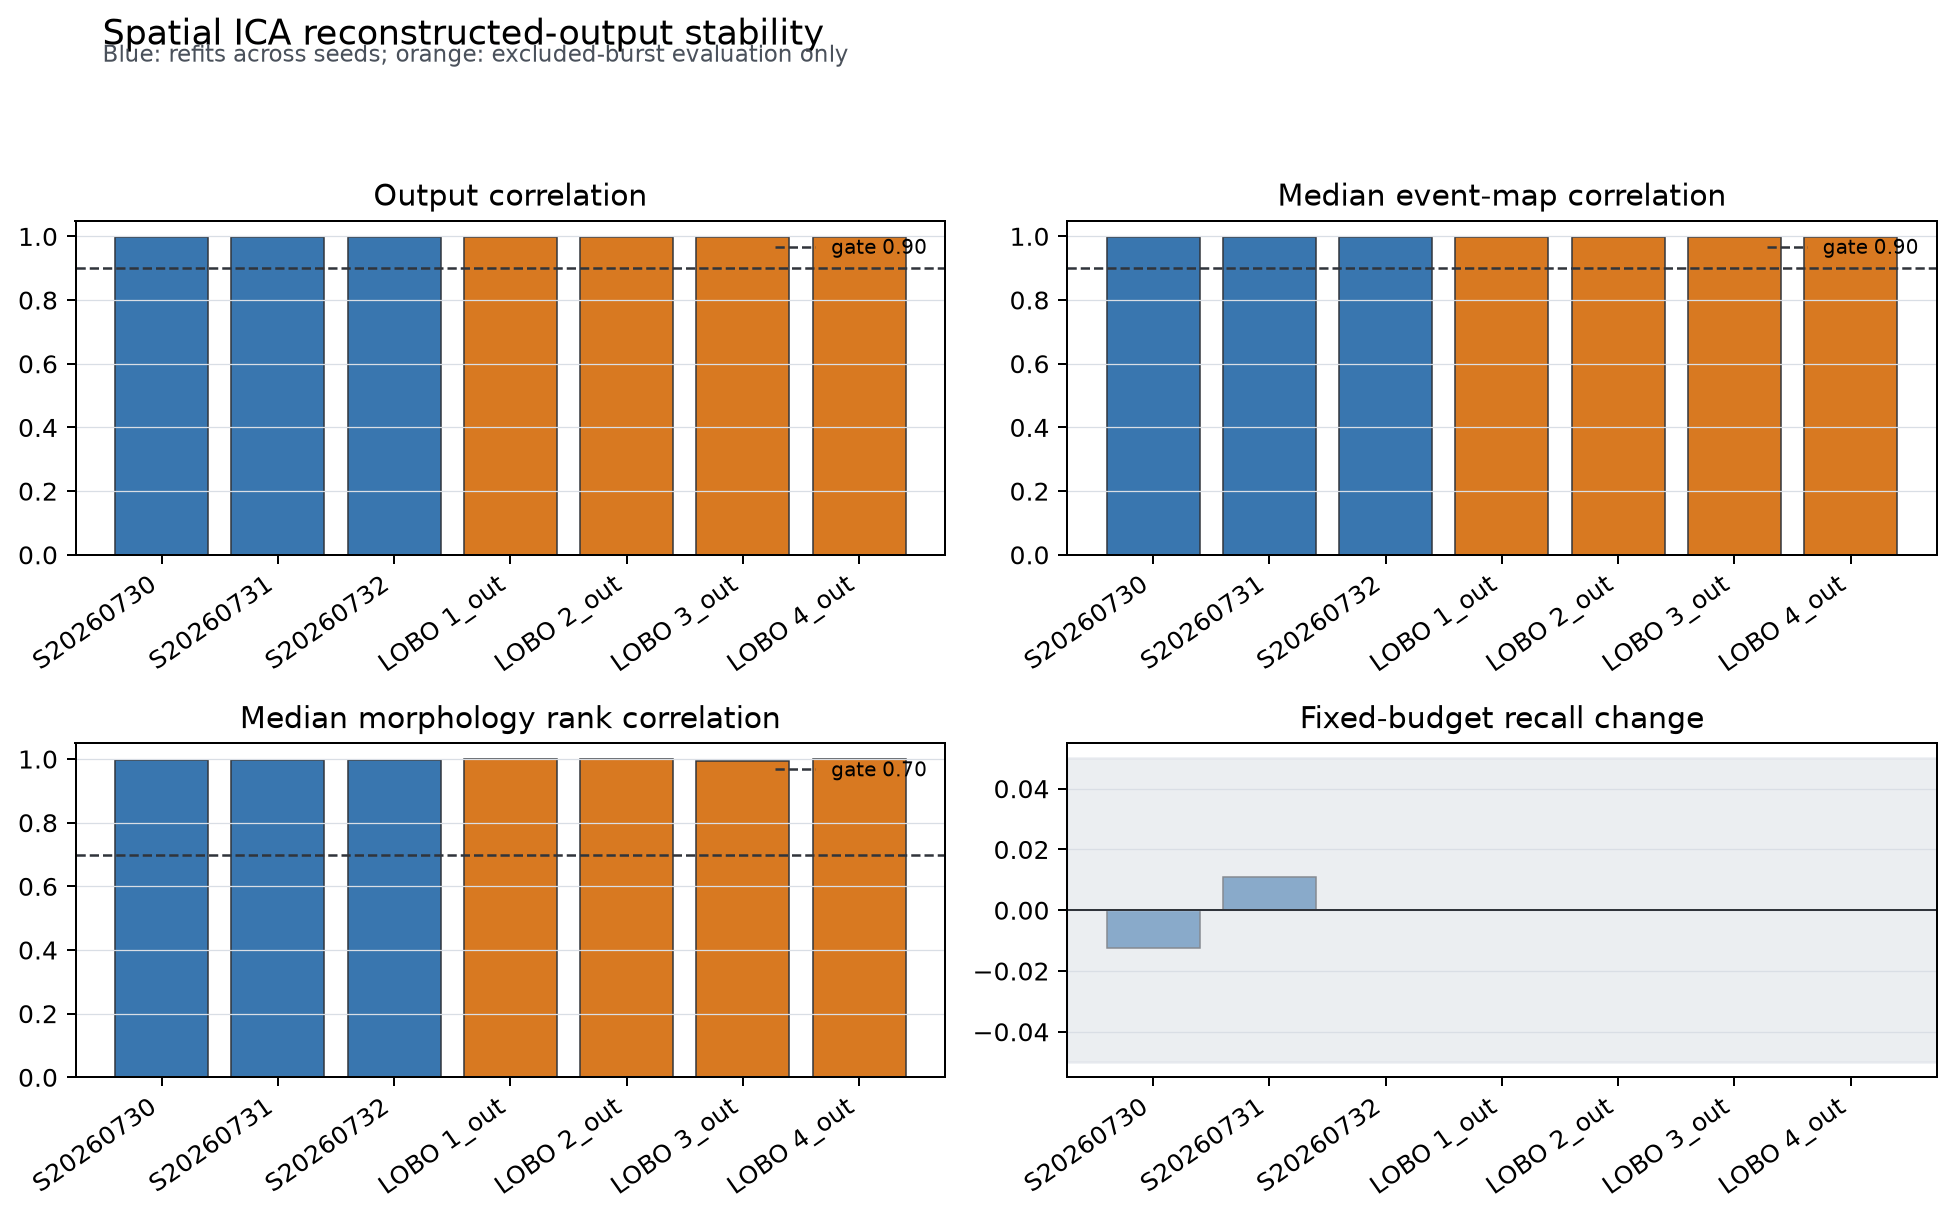
\includegraphics[width=0.98\linewidth]{figures/final/spatial_ica_reconstruction_stability.png}
  \caption{Spatial-ICA reconstructed-output stability across random seeds and leave-one-burst-window-out refits. Correlations, morphology-rank agreement, peak timing, and fixed-budget known-positive recall remained within the prespecified gates.}
  \label{fig:spatial-ica-reconstruction-stability}
\end{figure}

\subsection{Class and certainty alignment remain suggestive, not validated}

The 53 protected-v1 one-to-one matches collapsed to 17 immutable sites with dominant-class counts 7, 1, and 9. Only one Class~2 site made a protected three-class comparison inadmissible. Across 14 protected class--morphology tests, no spatial-ICA metric approached corrected significance; the two smallest corrected values ($q=0.0588$) were Raw contrast and Raw boundary sharpness, metrics partially overlapping the spatial-specificity feature used to fit the classes.

In candidate-assisted canonical v7, the 24 identities had dominant-class counts 3, 5, and 16. The strongest spatial-ICA association was boundary sharpness ($\epsilon^2=\SpatialICAVsevenBoundaryEpsilon{}$, nominal $p=0.00485$), but it did not survive the 14-test correction ($q=\SpatialICAVsevenBoundaryQ{}$). Its class medians were $-0.022$, $0.018$, and $0.263$, providing a concrete hypothesis for independent data rather than a confirmed class distinction.

Confirmed identities had dominant-class counts 3, 2, and 10, compared with 0, 3, and 6 for identity-uncertain identities. At the canonical-identity grain, the association was not supported (Cramer's $V=\CertaintyDominantClassCramersV{}$, permutation $p=\CertaintyDominantClassPermutationP{}$). After adjustment for class and burst, none of 14 Raw or spatial-ICA morphology metrics distinguished the 15 confirmed from nine uncertain identities after multiplicity correction, and every bootstrap interval included zero. The data therefore do not establish that the frozen classes or objective ICA morphology encode reviewer certainty.

\begin{figure}[!htbp]
  \centering
  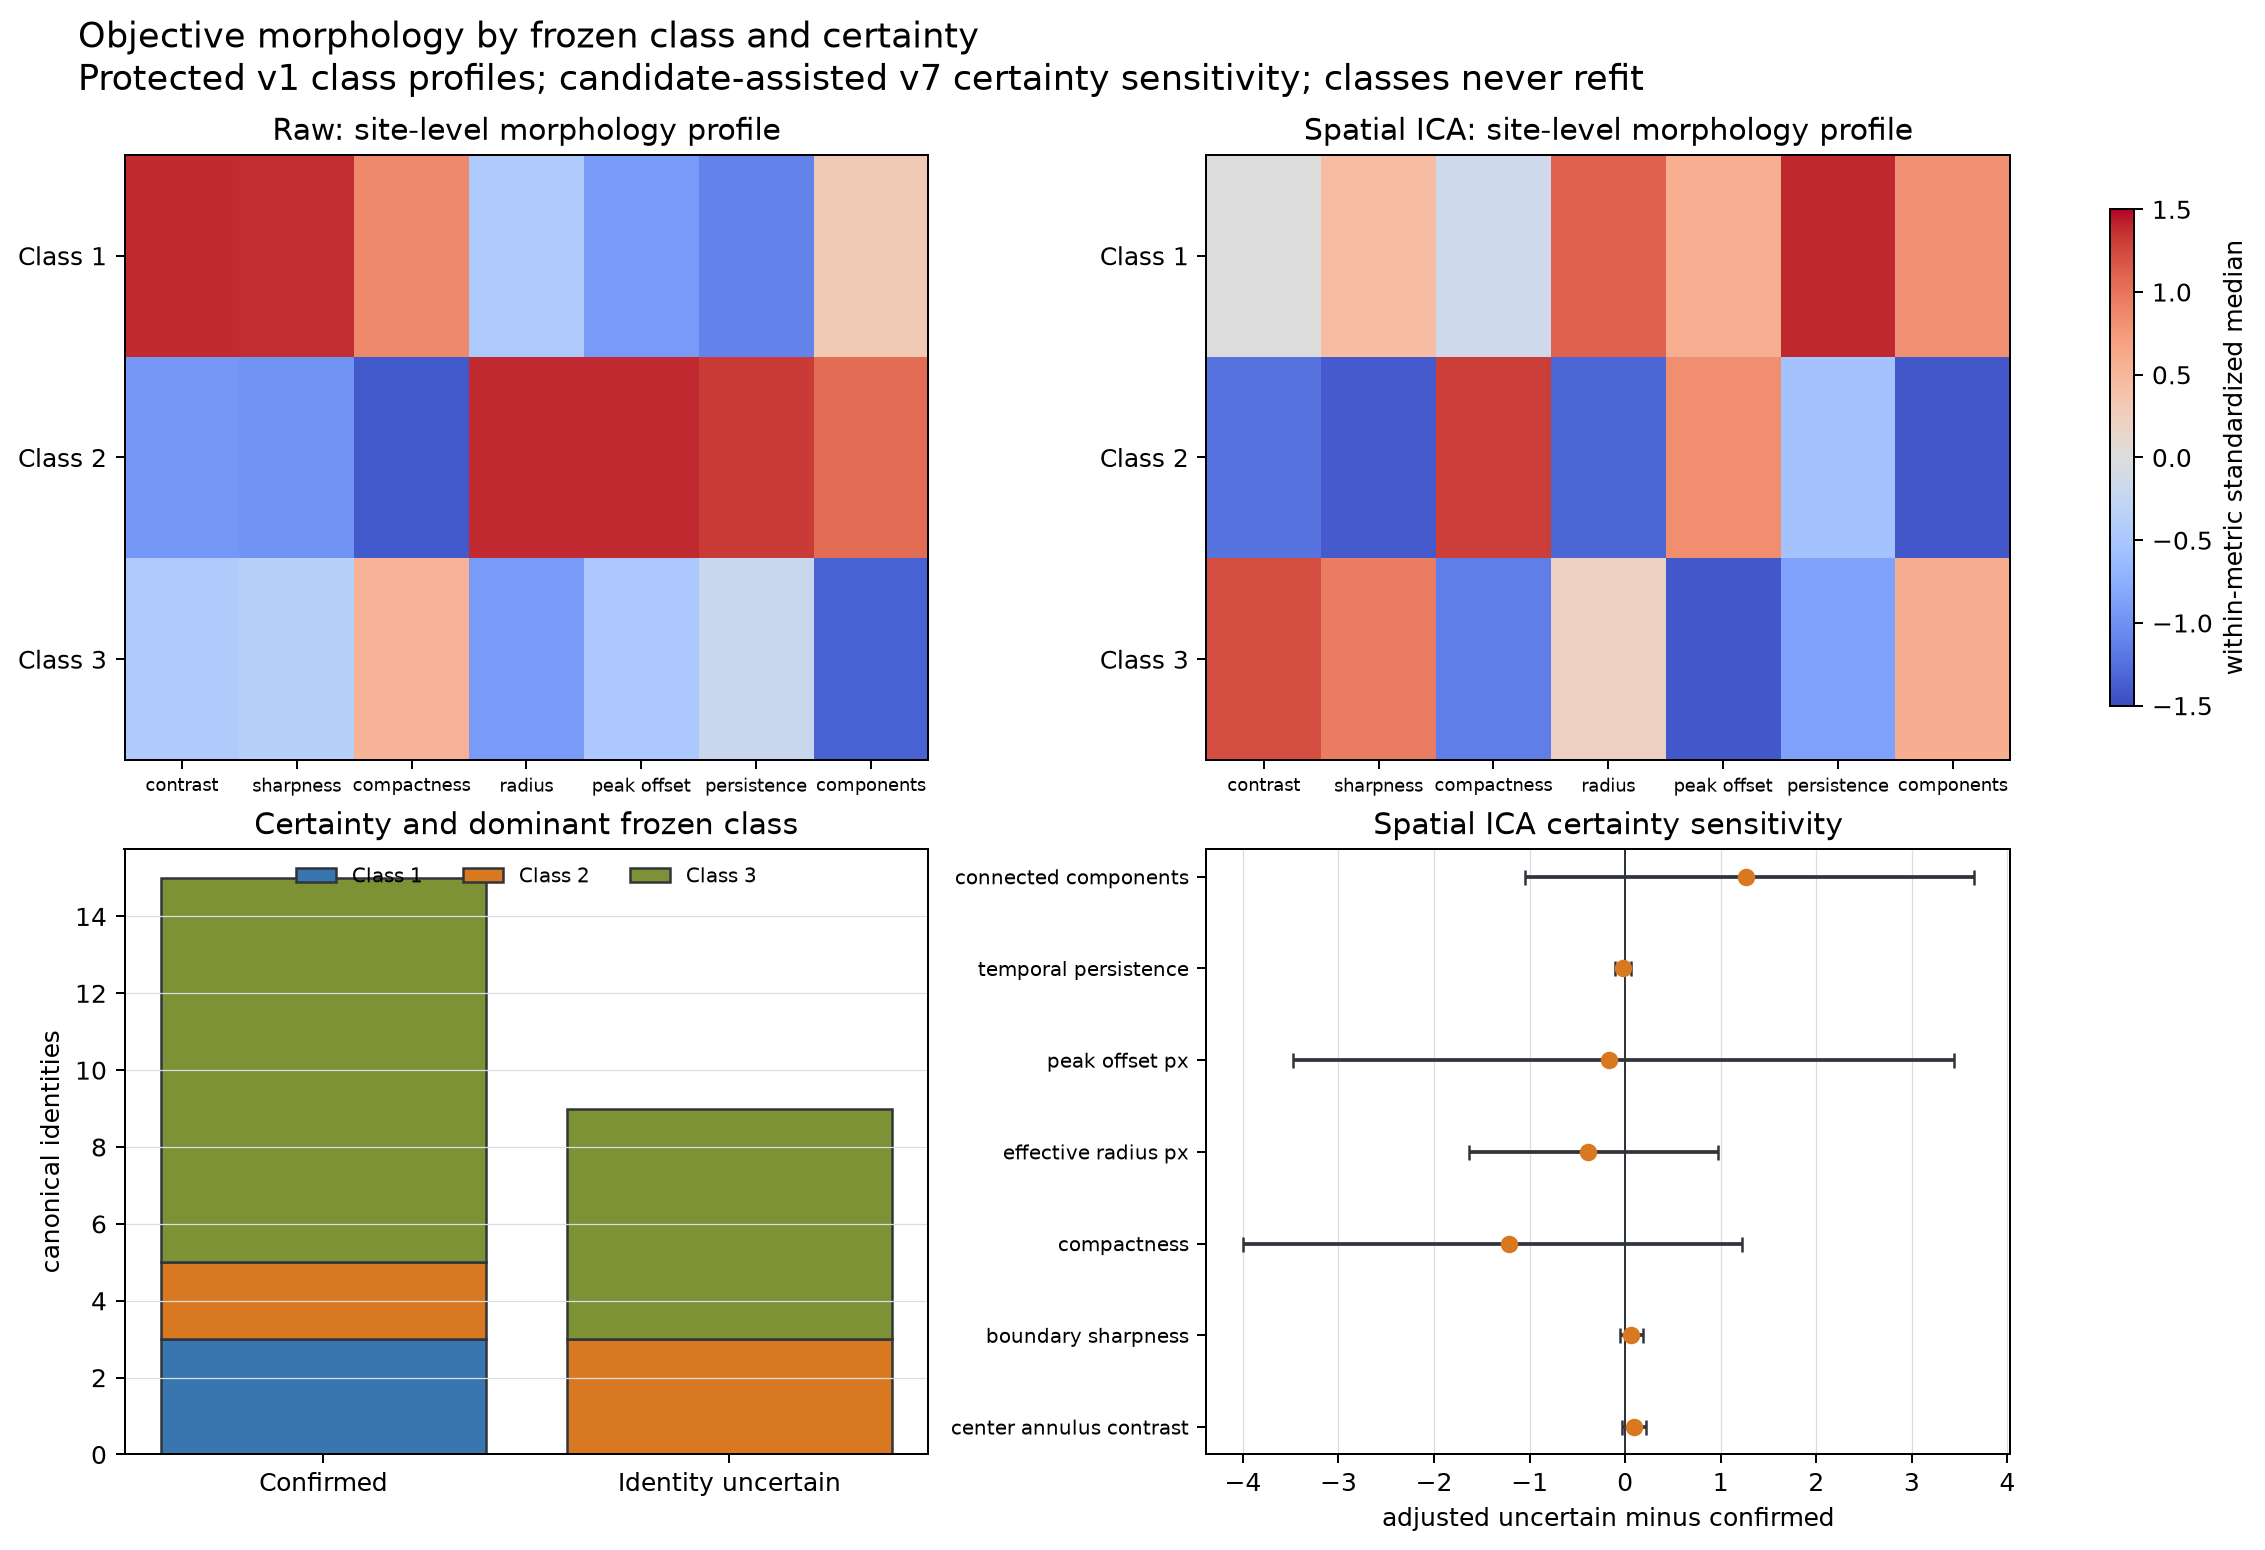
\includegraphics[width=0.98\linewidth]{figures/final/spatial_ica_class_certainty.png}
  \caption{Protected-v1 and canonical-v7 class/certainty alignment with objective morphology. Protected three-class inference is blocked by a single Class~2 site; canonical-v7 certainty comparisons are candidate-assisted and aggregated at canonical identity.}
  \label{fig:spatial-ica-class-certainty}
\end{figure}

\begin{figure}[!htbp]
  \centering
  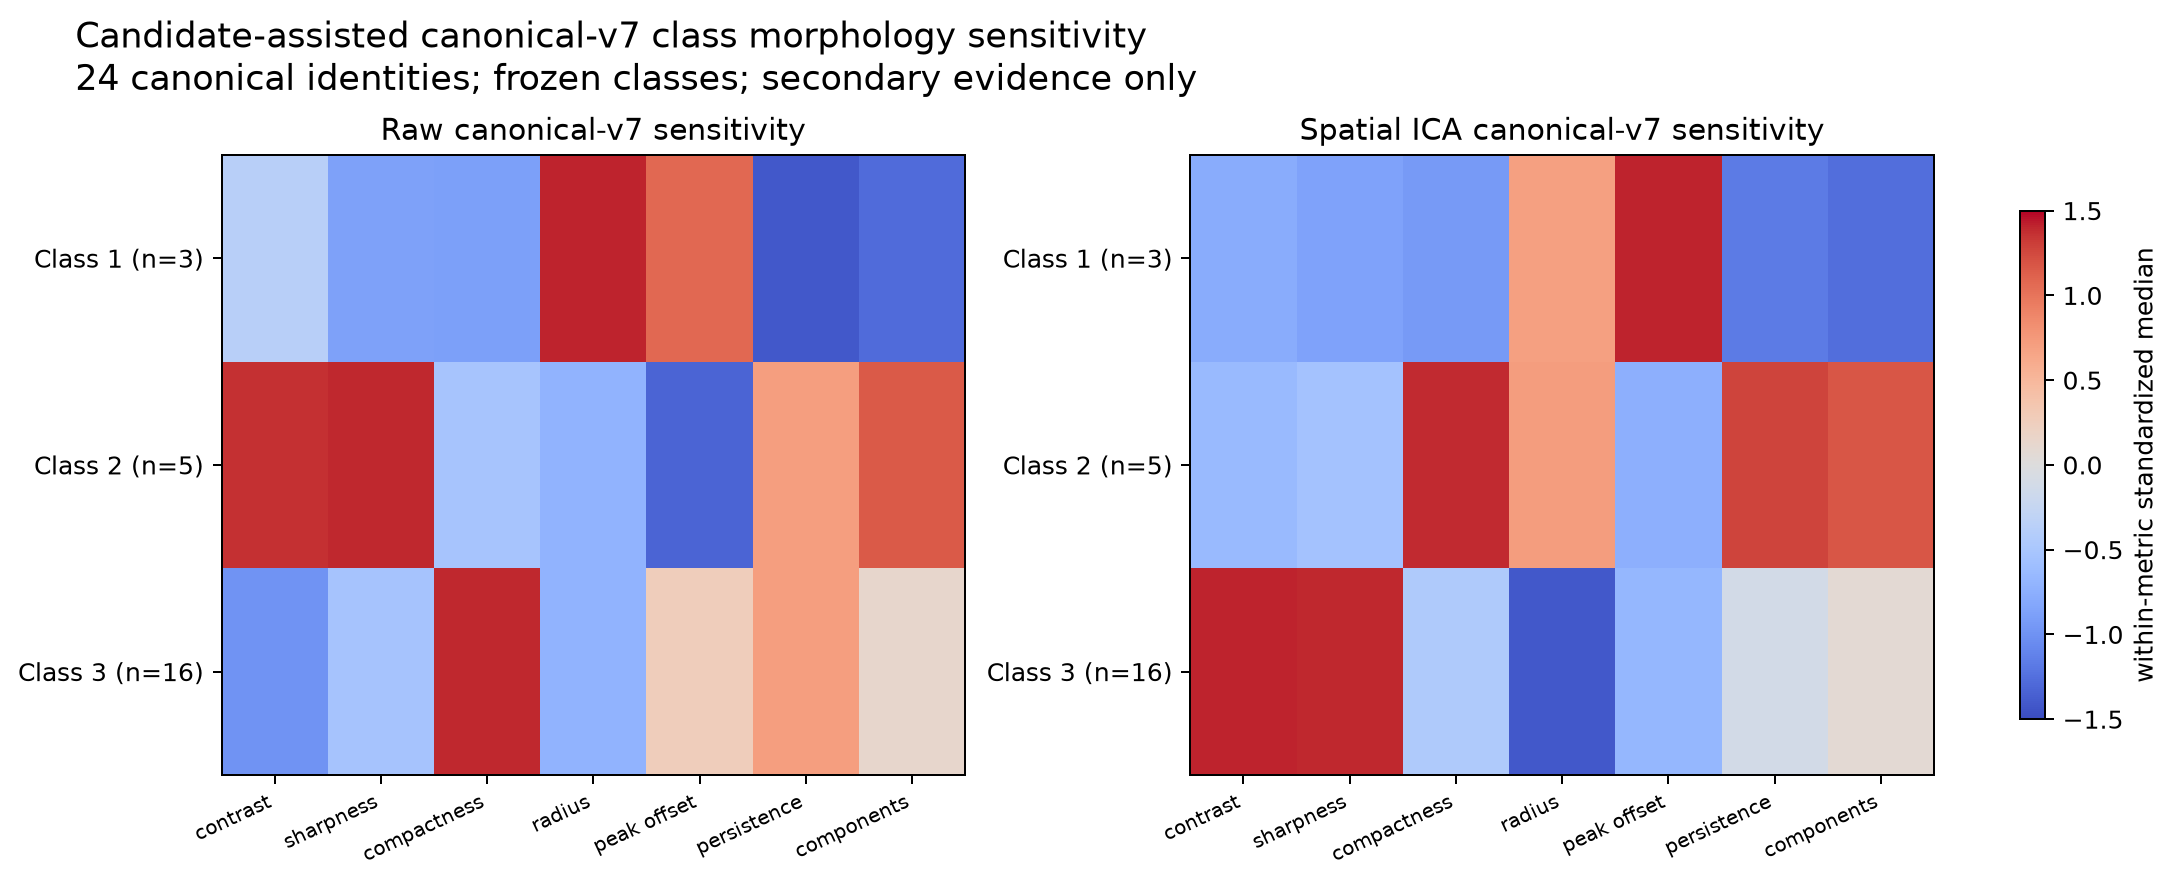
\includegraphics[width=0.98\linewidth]{figures/final/spatial_ica_canonical_v7_sensitivity.png}
  \caption{Candidate-assisted canonical-v7 sensitivity of objective morphology across dominant frozen classes. Spatial-ICA boundary sharpness is the strongest descriptive separation but does not survive family-wise false-discovery-rate control.}
  \label{fig:spatial-ica-v7-sensitivity}
\end{figure}

\subsection{Prespecified confirmatory hypotheses}

The protected rerun follows the hypothesis hierarchy in \Cref{tab:hypotheses}. Functional and tensor analyses are promoted only if trace completeness, held-out reconstruction, and component-stability gates pass. A null or heterogeneous result remains scientifically reportable because it defines the boundary between shared burst detection and neuron-specific identification.

\begingroup
\footnotesize
\setlength{\tabcolsep}{3pt}
\setlength{\LTpre}{0.4\baselineskip}
\setlength{\LTpost}{0.4\baselineskip}
\begin{longtable}{p{0.055\textwidth} >{\raggedright\arraybackslash}p{0.34\textwidth} >{\raggedright\arraybackslash}p{0.19\textwidth} >{\raggedright\arraybackslash}p{0.32\textwidth}}
\caption{Prespecified hypothesis hierarchy for the protected analysis.}\label{tab:hypotheses}\\
\toprule
ID & Hypothesis & Current status & Confirmatory decision rule \\
\midrule
\endfirsthead
\multicolumn{4}{l}{\small\itshape Table \thetable\ continued from previous page}\\
\toprule
ID & Hypothesis & Current status & Confirmatory decision rule \\
\midrule
\endhead
\midrule
\multicolumn{4}{r}{\small\itshape Continued on next page}\\
\endfoot
\bottomrule
\endlastfoot
H1 & Annotated events differ from matched ordinary times. & Supported provisionally. & Site/burst-aware block-shift effect and interval exclude the null region. \\
H2 & Event activity is spatially concentrated at the labeled site. & Partial amplitude evidence. & ROI contrasts outperform matched spatial controls; equivalence assessed only with frozen margins. \\
H3 & Sites or neurons possess stable activation gain/observability. & Strong exploratory motivation. & Cross-burst rank stability and site variance component pass preregistered reliability gates. \\
H4 & Neurons possess reproducible neuron-specific temporal waveforms. & Not established. & Functional site component improves held-out reconstruction and exceeds spatial controls. \\
H5 & Measurement phenotype explains known-positive recovery failures. & Suggestive. & Prespecified covariates improve held-out recovery model with stable coefficient direction. \\
H6 & Two-frame ICA adds information beyond temporal difference. & Provisionally rejected. & Promote only if repaired rerun breaks the analytic equivalence and adds utility/fidelity. \\
H7 & Compact spatial/contextual statistics add recovery information. & Supported provisionally. & Frozen same-proposal and proposal-union comparisons improve known-positive recall without disproportionate burden. \\
H8 & Directed or network interactions are identifiable. & Not established. & Exploratory only; no causal promotion from this recording. \\
\end{longtable}
\endgroup


\section{Discussion}
\label{sec:discussion}

\subsection{Change detection is not source identification}

The central methodological distinction in this study is between detecting temporal change and identifying a neuron-specific source. A two-frame operator can respond strongly at the onset of a burst while discarding slow fluorescence morphology or preserving activity that is equally visible in surrounding tissue. The near-equivalence between the learned ICA component and signed difference is therefore not merely a negative result. It identifies the operation that the learning procedure selected under this data geometry and prevents an unsupported interpretation of the component as an independently recovered neuronal signal.

This distinction is consistent with the evolution from PCA/ICA cellular-signal
sorting to modern modular calcium-imaging methods, which separately model
spatial footprints, temporal traces, background activity, and deconvolved
events \citep{mukamel2009automated,pnevmatikakis2016simultaneous,giovannucci2019caiman,zhou2018cnmfe}.
The appropriate comparison for NeuRev is not whether every representation
resembles one of these packages, but whether each proposed operator contributes
a measurable function: temporal-change sensitivity, spatial localization,
nuisance removal, waveform preservation, or candidate ranking.

\subsection{A shared burst waveform can coexist with local neuronal information}

The current evidence supports a strong event-aligned Raw waveform while showing that nearby tissue contains a similar morphology. This pattern is compatible with several mechanisms, including widespread neural recruitment, neuropil contamination, motion-coupled fluorescence, common illumination or acquisition dynamics, or spatially broad indicator responses. The data do not yet identify their relative contributions. Local annulus subtraction removes part of the shared component and leaves event-associated amplitude, but it can also suppress real spatially broad neural signal. Consequently, residualization should be evaluated as a measurement transformation, not assumed to yield ground truth.

The proposed functional and tensor decompositions make this ambiguity explicit. A dominant rank-one structure would support a shared temporal waveform modulated by site and burst gains. Reproducible additional components could indicate kinetic or spatial substructure, but they would still require matched spatial controls and held-out stability before being interpreted as neuron-specific. Conversely, failure to find stable additional components would bound the amount of neuron-specific waveform information identifiable from this recording.

\subsection{Feature value depends on where the search problem begins}

The new complete-trace panel and the earlier protected full-field screen address
different stages of the pipeline. Once a confirmed center is supplied, Raw and
carrier amplitude already place nearly every annotated event above every
same-duration quiet window, leaving little headroom for a more elaborate
transform. When the location is unknown and the candidate budget is scarce,
local coherence improves known-positive recovery by requiring neighboring
pixels to express compatible dynamics. This is consistent with correlation and
peak-to-noise seeding in CNMF-E and with the broader decomposition of spatial,
temporal, and background terms in CaImAn
\citep{zhou2018cnmfe,giovannucci2019caiman}.

This division argues for a compact role-specific stack. Amplitude should remain
the trace-level carrier; coherence should supply spatial proposal/ranking
evidence; lagged recurrence should remain secondary temporal context and must
not be interpreted causally. Annular subtraction and variance stabilization
remain valuable diagnostics, but local neuropil correction can either reduce
contamination or remove genuine shared activity and therefore requires
dataset-specific validation \citep{keemink2018fissa}. Likewise, the exponential
matched-filter comparator is not a substitute for generative spike inference.
Methods such as OASIS model calcium kinetics explicitly, while benchmarking
shows that performance depends on indicator, sampling, preprocessing, task
metric, and electrophysiological ground truth
\citep{friedrich2017oasis,berens2018benchmarking}.

The consensus and multiscale-persistence extensions are most interesting as
observability features. They do not improve event localization over the carrier,
but they retain measurable cross-burst site-rank variation after amplitude
percentiles saturate. That stability is hypothesis-generating evidence for a
site reliability profile, not confirmation of a neuronal phenotype. Because
the same recording motivated and evaluated the extensions, their definitions
must now be frozen and transferred without tuning to an independent recording.

The automated challenge suite narrows these roles further. Raw amplitude,
carrier, coherence, and recurrence remain strong under frame-level retrieval,
small timing shifts, and moderate coordinate displacement. A richer grouped
recovery model improves discrimination in point estimates, but the
site-bootstrap interval crosses zero; with only 12 primary misses, this is not
confirmatory feature complementarity. The high repeatability but weak retrieval
of annular contrast is an equally important warning: a stable statistic may
encode persistent local contamination or acquisition geometry rather than
useful event signal.

The subsequent deep dives make the engineering roles more concrete. Coherence
and lag produced much larger early-budget advantages in their native proposal
streams than when restricted to a common proposal universe, which argues
against treating them as rerankers alone. Lag added more repeated-split recovery
value than coherence, whereas the full role-specific stack remained the best
point estimate. A one-frame-rise, 20-frame-decay filter was selected in every
leave-one-burst-out fold, supporting a small kinetic bank as a transparent
alternative to a single arbitrary time constant. None of these results removes
the need for new recordings or bounded-field truth: only 12 all-lane misses are
available, and the proposal contrast is descriptive rather than causal.

The canonical-v8 identity-aware audit further shows why localization and
identity resolution cannot be collapsed into a single response-maximization
step. Eight of the 12 local consensus shifts entered the neighborhood of an
existing labeled geometry, including six shifts toward a different canonical
identity. The stronger shifted waveform may therefore belong to a neighboring
source rather than reveal a corrected center for the missed observation. This
supports joint footprint or assignment-aware localization and makes automatic
recentring an unsafe repair rule in crowded regions. The four identity-clear
cases remain useful targeted hypotheses, but noise, ranking, and
non-maximum-suppression still require separate adjudication.

The highest-value feature work is consequently identity-conditional. First,
the binary recovered-versus-missed outcome should be decomposed into recovered,
identity-clear miss, and identity-ambiguous collision. With only four
identity-clear misses, this is initially a descriptive or penalized model, not
a new confirmatory classifier. Second, spatial-offset vectors should be tested
for agreement across Raw, ICA, local standardization, and repeated bursts; a
stable direction supports localization error, whereas stage- or burst-specific
motion suggests contamination or acquisition drift. Third, point sampling
should be compared with fixed disks and footprint-weighted extraction to test
whether crescent, elliptical, or multi-lobed illumination explains fragile
center traces.

Fourth, crowded-field features should quantify the target-to-neighbor peak
ratio, nearest competing maximum, saddle depth, NMS suppression margin, and
local response-field topology. Fifth, original and candidate traces should be
regressed jointly on neighboring labeled traces. Large neighbor partial
correlation or a better nonnegative mixture fit would indicate source leakage
rather than successful recentering. Sixth, footprint morphology---including
eccentricity, solidity, convexity deficit, boundary sharpness, radial
asymmetry, and multi-lobe evidence---should be evaluated for repeatability and
incremental failure stratification. These tests use the existing movies and do
not require human labels for every candidate, but biological identity and
precision still require bounded review.

The expanded automated suite provides a stopping rule for incremental feature
engineering. The full panel clearly exceeds carrier-only internal prediction,
but its most stable feature is variance-stabilized annular context, which likely
combines observability, background, and acquisition geometry. Multiscale
persistence and lag recurrence add complementary context, whereas a simple
distance graph does not explain recovery. The next scientific gain is therefore
unlikely to come from another small transform on the same bursts. It requires a
change in evidence regime: independent-recording transfer, bounded
identity-complete truth, or a realistic movie generator with exact source
identity.

These results match the modular logic of established calcium-imaging methods,
which distinguish spatial filtering or footprints from temporal calcium
dynamics and background terms
\citep{vogelstein2010deconvolution,pnevmatikakis2016simultaneous,giovannucci2019caiman}.
They do not show that the present compact operators recover spikes or demixed
sources. Realistic simulation frameworks add anatomy, optical propagation,
motion, indicator kinetics, and sensor noise and can expose false positives
that strong extracted time courses alone do not reveal \citep{song2021naomi}.
The monotonic one-dimensional injection result therefore justifies retaining
the matched filter for transfer testing, while also defining why movie-level
simulation is the next synthetic step.

\subsection{Stable observability may be the most productive neuron-level target}

Detailed activation morphology need not be the only reproducible property of a neuron. A site may repeatedly exhibit high amplitude, strong SNR, compact spatial support, weak annulus coupling, or reliable candidate ranking even when its exact waveform varies. We refer to this profile as a measurement or observability phenotype. The term is deliberately nonbiological: stable visibility can arise from expression level, optical depth, focus, cell size, local crowding, acquisition field, or true response magnitude.

Quantifying observability has direct methodological value. It can explain why some known neurons are systematically recovered while others are repeatedly missed, reveal whether apparent algorithm failures are actually proposal or acquisition failures, and guide the next annotation or data-collection effort. A detector that improves only for already bright, isolated neurons is less scientifically useful than one that expands coverage of difficult but credible sites. The proposed variance-component and recoverability models therefore treat site-associated heterogeneity as a primary result rather than nuisance variation.

\subsection{Incomplete annotation changes what detection metrics mean}

Sparse positive labels make recall of known observations identifiable but leave full-field precision unidentified. Treating every unmatched candidate as background would penalize the algorithm for discovering neurons omitted by the annotation process and would favor conservative methods that reproduce the labeling bias. Positive--unlabeled learning theory emphasizes that conclusions depend on how positives enter the labeled set, particularly when labeling is not random \citep{bekker2020pu}.

The bounded-field annotation study is designed to convert one small region from positive--unlabeled to exhaustively reviewed data. Its value is disproportionate to its size: it permits a local precision estimate, a false-candidate taxonomy, an estimate of hidden-positive prevalence, and an assessment of whether candidate score calibrates review confidence. The rest of the full field remains useful for known-positive recovery and discovery, but it should not be assigned a fictitious negative class.

\subsection{Implications for unsupervised learning in NeuRev}

Avoiding large supervised models is appropriate given the current data volume, but unsupervised learning does not remove the need for scientific evaluation. An unsupervised representation can learn acquisition structure, global burst timing, local covariance, or a simple derivative. The relevant question is whether it exposes a stable and useful statistic that an interpretable comparator does not already provide.

The confirmatory program therefore places learned and analytic operators in the same frozen panel. Pairwise ICA remains as an equivalence control; local coherence and lagged recurrence are tested for ranking utility; residualization is tested for spatial specificity and fidelity; and Raw remains the carrier against which information loss is measured. New learning is warranted only when the existing analysis identifies a missing operation or a reproducible residual structure that cannot be represented by the compact panel.

For subsequent max-envelope studies, we distinguish
\emph{causal local standardized surprise} (the existing LS/MSLN output) from
\emph{positive instantaneous evidence} at the current frame and coordinate,
its \emph{contextual upper envelope} over a declared causal support, and their
\emph{envelope agreement}. The resulting product is termed
\emph{envelope-gated evidence}; multiplying instantaneous evidence by envelope
agreement gives \emph{agreement-attenuated evidence}. This vocabulary is
operator-specific and deliberately does not rename the established
\emph{local coherence} feature, which remains a causal pixel-to-neighborhood
correlation. The bounded pilot defining these terms is non-claim-bearing and
does not establish detection utility. In the subsequent all-occurrence
comparison, temporal agreement attenuation was effectively indistinguishable
from amplitude squaring under peak-localization ranking, whereas adding a
3-by-3 spatial envelope reduced known-center localization, especially after
temporal-envelope-to-LS-to-ICA processing. This follows from the operator and
estimand: at a local maximum included in its causal envelope, the upper
envelope equals the instantaneous evidence and the attenuation vanishes.
Temporal agreement attenuation should therefore remain a morphology-sensitive
diagnostic unless it succeeds under integrated-energy, duration, or bounded
full-field specificity endpoints.

A subsequent visual-first morphology audit confirms that this caution should
not be mistaken for rejection of temporal pooling. Across all 106 confirmed
occurrences, the five-frame upper envelope broadened and prolonged event
evidence, whereas agreement-attenuated evidence preserved the aligned peak,
increased core concentration, and reduced the post-peak shoulder in Raw and
both learned representations. Envelope-gated evidence produced stronger event
concentration but behaves partly as an amplitude-emphasizing transform. These
operators therefore have different potential product roles: short causal
memory, proposal reinforcement, and peak-preserving temporal sharpening. They
remain within-recording measurement features; whether any improves candidate
specificity requires bounded-field truth, and waveform analyses must preserve
the unattenuated carrier because attenuation deliberately changes decay shape.

The spatial-ICA results sharpen this conclusion. Individual filters varied too much across seeds and held-burst exclusions to support component-wise anatomical interpretation, yet dense reconstruction was nearly invariant and preserved event-map morphology, peak timing, and known-positive recall. Basis instability and representation stability are not contradictory: multiple rotated or redistributed bases can span a similar useful signal subspace. For annotation, spatial ICA can remain a useful visual and quantitative representation without implying that any displayed component is a uniquely identifiable neuron.

Objective translated-control comparisons support localized morphology at labeled coordinates, but they do not turn sparse positives into exhaustive truth. Likewise, the class analyses provide plausible structure---especially the candidate-assisted boundary-sharpness gradient---without corrected evidence that the classes encode spatial-ICA morphology or reviewer certainty. The frozen classes should remain measurement-event archetypes rather than neuron types.

\subsection{Limitations}

The study has several non-negotiable limitations. First, one recording cannot establish generalization across animals, preparations, sessions, or microscopes. Second, four shared bursts provide limited independent temporal replication and make burst-level variance estimates imprecise. Third, current labels are sparse and partly uncertain, and the same bursts have informed multiple exploratory decisions. Fourth, pre-repair identity-sensitive numbers remain provisional even though later analyses preserve immutable site geometry. Fifth, annulus subtraction is not a pure nuisance-removal operation. Sixth, candidate-based metrics outside the bounded field cannot identify precision or specificity. Seventh, any coactivity or lag analysis is descriptive because shared drive and calcium kinetics can generate apparent network structure. Eighth, the spatial-ICA fit is transductive within one recording, its positive encoding clips negative reconstructed values, and its manual review panel has been deferred; objective morphology and reconstruction stability do not establish reviewer utility or biological source separation. Ninth, the complete-trace panel conditions on confirmed centers and reuses previously analyzed bursts; its ceiling-limited event-localization metric neither validates the two new features nor ranks their full-field specificity. Tenth, the automated recovery model has only 12 primary misses and its improvement interval crosses zero. Eleventh, circular shifts and simplified trace injections validate alignment and operator behavior but do not reproduce anatomy, optics, motion, or biological ground truth. Twelfth, the canonical-v8 recentering candidates are response-selected within the same recording, and the identity guard uses sparse labeled geometry rather than exhaustive biological source truth.

\begin{table}[!htbp]
\centering
\caption{Limitations and the corresponding manuscript safeguard.}
\label{tab:limitations}
\small
\begin{tabularx}{\linewidth}{>{\raggedright\arraybackslash}p{0.30\linewidth} X}
\toprule
Limitation & Safeguard \\
\midrule
One canonical recording & Restrict claims to within-recording measurement structure; require an independent recording for external generalization. \\
Four shared burst intervals & Use leave-one-burst-out and burst-exclusion sensitivity; avoid asymptotic burst-level claims. \\
Sparse, partly uncertain positives & Use positive--unlabeled metrics and preserve confidence/provenance; estimate precision only in a bounded exhaustive field. \\
Identity/geometry collision in existing assays & Repair before trace aggregation; preserve original sites and regenerate all identity-sensitive results. \\
Response-selected recentering can transfer identity & Require nearest-label and footprint-assignment guards; never count a stronger shifted trace as recovery by itself. \\
Repeated exploratory use of the same bursts & Freeze the compact panel and estimands before a protected confirmatory rerun. \\
Local annulus may contain true neural signal & Report Raw, annulus and residual jointly; treat subtraction as a transformation, not ground truth. \\
Acquisition heterogeneity and saturation & Characterize noise, field effects, motion and saturation before interpreting stable observability. \\
Shared drive can induce network correlations & Keep connectivity analyses descriptive and condition on global/local common mode. \\
\bottomrule
\end{tabularx}
\end{table}


These limitations do not make the dataset scientifically unusable. They determine the level at which it should be analyzed. The strongest contribution is a transparent within-recording measurement study, accompanied by explicit criteria for the additional data and annotation required to promote each claim.

\subsection{Highest-value next evidence}

The most valuable immediate addition is not a wider hyperparameter sweep. It
is exhaustive review of one bounded field using the frozen carrier, coherence,
and recurrence panel, so proposal coverage, ranking, and precision can be
separated. The most valuable future dataset is an independently acquired
recording that satisfies a frozen quality and annotation contract. Such a
recording would test the shared-versus-specific decomposition and determine
whether the consensus and multiscale-persistence site rankings transfer without
retuning. For synthetic work, an anatomy- and optics-aware movie simulation is
more informative than further widening the present one-dimensional injection
grid.

\section{Conclusion}
\label{sec:conclusion}

Sparse zebrafish fluorescence data require a distinction between event detection, spatial localization, source identification, and biological interpretation. The NeuRev evidence is most coherent when framed as a measurement and identifiability study: temporal differentiation detects burst-associated change; Raw traces contain a strong shared waveform; local subtraction retains event-associated amplitude; and spatial ICA provides a localized, highly stable reconstructed representation despite unstable individual filters. At confirmed centers, amplitude already localizes the bursts nearly perfectly over the complete trace; local coherence adds its clearest value earlier, during full-field proposal and scarce-budget ranking. Consensus and multiscale persistence are promising only as exploratory cross-burst observability features. Automated displacement, perturbation, circular-shift, and injection tests show that the compact features contain localized and event-aligned measurement structure, while grouped recovery modeling stops short of confirming incremental utility. Frozen measurement-event classes recur across bursts, but current data do not establish their alignment with spatial-ICA morphology or reviewer certainty. By preserving spatial-site identity, respecting positive--unlabeled labels, assigning features to task-specific roles, and reserving precision for exhaustively reviewed data, the framework converts a data-limited detection problem into a sequence of falsifiable scientific questions. Realistic synthetic movies, bounded-field truth, and independent-recording transfer are now higher priorities than further same-recording feature expansion.

\section*{Declaration of competing interests}
\AuthorDecision{Confirm that the authors have no competing financial or personal interests, or provide the required disclosure.}

\section*{Ethics statement}
\AuthorDecision{Insert the animal-use protocol, approving institution, protocol number, and confirmation that procedures followed applicable guidelines. Do not infer these details from the repository.}

\section*{Funding}
\AuthorDecision{List funding sources, grant numbers, and the role of each funder.}

\section*{CRediT authorship contribution statement}
\AuthorDecision{Complete CRediT roles for every author. Suggested roles to review include Conceptualization, Methodology, Software, Validation, Formal analysis, Investigation, Data curation, Visualization, Writing--original draft, Writing--review \& editing, Supervision, Project administration, and Funding acquisition.}

\section*{Data availability}
The release manuscript will cite a versioned data and annotation package or state the access restrictions and their justification. At minimum, the package will include immutable observation identifiers, site geometry, canonical-identity decisions, burst intervals, annotation provenance, configuration files, source hashes, generated result macros, and a figure/table source map. \AuthorDecision{Select public repository/accession, controlled-access process, or justified non-release statement.}

\section*{Code availability}
The analysis code will be released from a versioned NeuRev Workbench revision together with an executable environment specification and the protected-run configuration. \AuthorDecision{Insert repository URL, release tag, and archival DOI when available.}

\section*{Acknowledgements}
\AuthorDecision{Acknowledge data collectors, annotators, imaging collaborators, laboratory support, and computing resources.}

\section*{Declaration of generative AI and AI-assisted technologies in the writing process}
During manuscript preparation, the authors used OpenAI language-model tools to help organize the analysis plan and draft a manuscript skeleton. The authors are responsible for verifying all text, code, citations, numerical results, and interpretations and will review and edit the final submission. \AuthorDecision{Revise this disclosure to match the journal's submission form and the tools actually used in the final manuscript.}


\appendix
\section{Manuscript result-status convention}
\label{app:result-status}
Values marked with a dagger are imported from pre-repair repository artifacts and are provisional. They must be regenerated after the observation-site/canonical-identity repair. The final manuscript build must fail if a provisional macro remains enabled.

\bibliographystyle{elsarticle-harv}
\bibliography{references}

\end{document}
